\chapter{Lattice excitations}\label{chap:11}
Below about \SI{10}{MeV} the largest free recoil energy that a nucleon-coupled dark-matter particle gives a silicon nucleus falls to the phonon energies, and the nucleus can no longer be treated as free. At that mass the largest momentum transfer is about \SI{50}{keV}, the free recoil energy $q^2/2M$ is \SI{50}{meV}, equal to the energy of the phonons themselves. Lighter particles give the nucleus less than one phonon's worth of energy, and the deposited energy goes into the lattice instead of into a free recoil. At the lowest masses it goes into a single acoustic or optical phonon, at intermediate masses into a few phonons, and only at the top of the range into a recoil broadened by the motion of the nucleus in its well. The electronic channels of \cref{chap:10} need an electron to cross a gap of an eV; the lattice channels need only a phonon of a few meV, and with a meV threshold they reach masses fifty times smaller than the electronic channels do. What is the rate, across that whole range, and which numbers of a material decide it?

From the harmonic crystal of \cref{chap:5} and the master formula of \cref{chap:8}, each regime of \cref{fig:11-map} reduces to a few material numbers: sound speeds, Born effective charges and Debye--Waller exponents, and each reduced rate is checked against a fuller calculation. Throughout, the electrons stay in their ground state and follow the nuclei. The Migdal effect and phonon-assisted electron recoil start from the lattice sector of this chapter and follow in \cref{chap:12,chap:13}.

\begin{figure}[tbp]
  \centering
  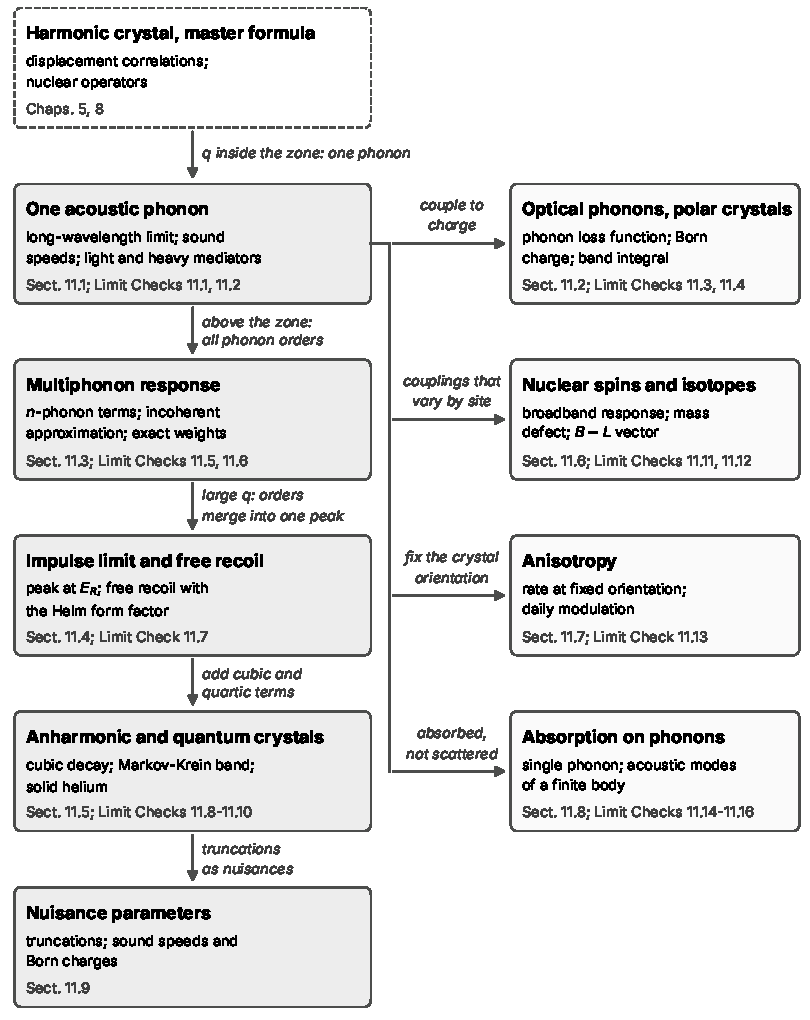
\includegraphics[width=0.85\linewidth]{figures/ch11/map11.pdf}
  \caption{The lattice regimes of the nuclear response and their branches. Left, as the momentum transfer grows: one acoustic phonon inside the zone (\cref{sec:11.1}; \cref{lim:11.1a,lim:11.1b}); all phonon orders at momentum transfers beyond the zone (\cref{sec:11.3}; \cref{lim:11.3a,lim:11.3b}); the orders merging into one peak at $E_R$, whose limit is the free nuclear recoil (\cref{sec:11.4}; \cref{lim:11.4a}); cubic and quartic terms (\cref{sec:11.5}; \cref{lim:11.5a,lim:11.5c,lim:11.5b}); the uncertainty budget of these rates (\cref{sec:11.9}). Right: coupling to charge excites optical phonons of polar crystals (\cref{sec:11.2}; \cref{lim:11.2a,lim:11.2b}); couplings that vary from site to site, nuclear spins and isotopes (\cref{sec:11.6}; \cref{lim:11.6a,lim:11.6b}); a crystal of fixed orientation and the daily modulation (\cref{sec:11.7}; \cref{lim:11.7a}); and absorption on phonons and acoustic modes (\cref{sec:11.8}; \cref{lim:11.8a,lim:11.8b,lim:11.8c}).}
  \label{fig:11-map}
\end{figure}

\section{Acoustic phonons}\label{sec:11.1}

A dark-matter particle of \SI{100}{keV} transfers at most $2\mchi v_{\mathrm{max}} = \SI{0.53}{keV}$ of momentum. Given to a free silicon nucleus, that momentum would deposit $q^2/2M = \SI{5.4}{\micro eV}$, far below any threshold. Given to the crystal, it can create one longitudinal acoustic phonon of energy $c_{\mathrm{LA}}q \approx \SI{16}{meV}$, because the whole crystal takes up the momentum and the energy is set by the sound speed rather than by the mass of a nucleus. The kinematic match, with the momentum taken up by the whole crystal and the energy set by the sound speed, makes single phonons the channel of the lightest dark matter that couples to nucleons (\cref{sec:1.3}). At long wavelengths the single-phonon rate depends on the material only through the sound speeds, and for a light mediator it is the same for every material.

\subsection{The one-phonon response}

Take a dark-matter particle that couples to protons and neutrons with the same potential $\tilde V_N(\vect{q})$, the spin-independent coupling $\mathcal{O}_1$ of \cref{sec:8.1}. By \cref{eq:8.1-nuclear}, a nucleus of species $\kappa$ then carries the coupling $A_\kappa\tilde V_N(\vect{q})F_N(q)$, and the dark matter sees the target through the single operator
\begin{equation*}
  O_N(\vect{q}) = \sum_\kappa A_\kappa\,n_\kappa(\vect{q}) ,
\end{equation*}
the nucleon number density of the crystal at momentum $\vect{q}$. The nuclear form factor $F_N$ of \cref{eq:2.2-FN} is one to better than $10^{-3}$ at the momentum transfers of this section, which stay below a few keV, and we drop it. The coupling has no electronic row, so the electrons enter only through the forces they transmit between nuclei: the phonons are those of the Born--Oppenheimer surface (\cref{sec:5.1}), and the final states lie in the electron-following sector of \cref{tab:8-sectors}. Screening, which acts on rows that couple to charge (\cref{sec:8.4}), does not enter. The dark photon, which couples to charge, is the subject of \cref{sec:11.2}.

The rate per unit target mass is \cref{eq:8.2-spectrum} with one row, $\mathfrak{D} = |\tilde V_N(\vect{q})|^2$ and $S = S_A$. Here $\omega_{\vect{q}} = \vect{q}\cdot\vect{v} - q^2/2\mchi$ is the energy the dark matter loses (\cref{eq:1.3-omegaq}), not a phonon frequency, and $S_A$ is the response \cref{eq:4.2-Sab} of $O_N$, the nuclear block $\sum_{\kappa\kappa'}A_\kappa A_{\kappa'}S_{\kappa\kappa'}$. The one-phonon part of $S_A$ follows from the amplitude of \cref{sec:5.3}. To first order in the displacement, a nucleus of species $\kappa$ emits a phonon $\vect{Q}\nu$ with the amplitude
\begin{equation*}
  \langle n_{\vect{Q}\nu} + 1|\,n_\kappa(\vect{q})\,|n_{\vect{Q}\nu}\rangle = \ii\,\ee^{\ii\vect{q}\cdot\vect{\tau}_\kappa}\,\frac{\vect{q}\cdot\vect{e}_{\kappa\nu}(\vect{Q})^*}{\sqrt{2M_\kappa\omega_{\vect{Q}\nu}}}\,\sqrt{N(n_{\vect{Q}\nu} + 1)}\,\sum_{\vect{G}}\delta_{\vect{q},\vect{Q} + \vect{G}} .
\end{equation*}
Keeping the full exponential of the displacement multiplies this amplitude by $\ee^{-W_\kappa(\vect{q})}$: to first order in the displacement correlation $\mathcal{C}_{\kappa\kappa'}$, the generating formula \cref{eq:5.6-gen} for a pair of nuclei is the one-phonon term with the factor $\ee^{-W_\kappa - W_{\kappa'}}$ in front. The amplitudes of the nuclei of one cell add with their phases. We square, sum over the final phonon states and divide by the volume $\Vol = N\Omega$ as in \cref{eq:4.2-Sab}. The factor $N$ cancels, and the Kronecker delta leaves in each branch one phonon wavevector $\vect{Q}$, the reduction of $\vect{q}$ to the first Brillouin zone:
\begin{keyresult}[One-phonon nuclear response]
\begin{equation}
  \begin{aligned}
  S^{(1)}_A(\vect{q},\omega) = \frac{2\pi}{\Omega}\sum_\nu{}&\frac{\bigl|\sum_\kappa A_\kappa\,\ee^{-W_\kappa(\vect{q})}\,\ee^{\ii\vect{q}\cdot\vect{\tau}_\kappa}\,\vect{q}\cdot\vect{e}_{\kappa\nu}(\vect{Q})^*/\sqrt{M_\kappa}\bigr|^2}{2\omega_{\vect{Q}\nu}} \\
  &\times\Bigl[(n_{\vect{Q}\nu} + 1)\,\delta(\omega - \omega_{\vect{Q}\nu}) + n_{\vect{Q}\nu}\,\delta(\omega + \omega_{\vect{Q}\nu})\Bigr] ,
  \end{aligned}
  \label{eq:11.1-S1}
\end{equation}
with $\vect{Q} = \vect{q} - \vect{G}$ in the first zone, $\vect{q}$ itself unreduced in the phase $\ee^{\ii\vect{q}\cdot\vect{\tau}_\kappa}$, and the phase convention of \cref{eq:5.3-u}.
\end{keyresult}
\noindent The absorption term follows from the second matrix element of \cref{eq:5.3-me}; since $\vect{e}_{\kappa\nu}(-\vect{Q}) = \vect{e}_{\kappa\nu}(\vect{Q})^*$, the modulus of the amplitude is unchanged. In a detector at \SI{10}{mK}, $n_{\vect{Q}\nu}$ vanishes for every phonon above a few tens of \si{\micro eV} (\cref{sec:5.3}), and only emission remains. On the truncation label of \cref{sec:8.5}, \cref{eq:11.1-S1} is the point $\mathcal{K}$ = one-phonon, $n_A = 0$, with $n_T = 0$ for the emission term and $n_T = 1$ for the absorption term, and $n_B = 0$ throughout.

The weight of a branch in \cref{eq:11.1-S1} is the projection of $\vect{q}$ on the displacement of each nucleus, divided by the phonon energy, so that soft modes polarized along $\vect{q}$ dominate. The momentum is conserved up to a reciprocal-lattice vector, so that each $\vect{q}$ excites one phonon per branch, with the energy fixed by the dispersion: the response is a set of sharp lines in $\omega$ at fixed $\vect{q}$. And the Debye--Waller factor $\ee^{-2W_\kappa}$ of \cref{eq:5.6-W} measures the competition with the multiphonon terms of \cref{sec:11.3}. In silicon, $2W_\kappa = q^2\langle u_x^2\rangle$ is $3\times10^{-3}$ at $q = \SI{2.25}{keV}$ with the zero-temperature $\langle u_x^2\rangle = \SI{2.45e-3}{\angstrom^2}$ of \cref{we:5-dw}, so in the first Brillouin zone the factor is one to $3\times10^{-3}$.

\subsection{The long-wavelength limit}

Most of the rate of light dark matter comes from momentum transfers well inside the first zone. For a crystal with a lattice constant of a few \si{\angstrom}, the scale of the zone is
\begin{equation}
  q_{\mathrm{BZ}} = \Bigl(\frac{6\pi^2}{\Omega}\Bigr)^{1/3} ,
  \label{eq:11.1-qBZ}
\end{equation}
the radius of a sphere with the volume of the Brillouin zone, which holds one wavevector per primitive cell. For silicon, $\Omega = a^3/4$ and $q_{\mathrm{BZ}} = \SI{1.139}{\angstrom^{-1}} = \SI{2.25}{keV}$, between the distances from $\mathrm{\Gamma}$ to L (\SI{1.98}{keV}) and to X (\SI{2.28}{keV}). The zone scale $q_{\mathrm{BZ}}$ should not be confused with the Debye wavevector $Q_{\mathrm{D}}$ of \cref{eq:5.2-debye}, which counts one wavevector per atom and is larger by $n_{\mathrm{at}}^{1/3}$.

For $q \ll q_{\mathrm{BZ}}$, \cref{sec:5.2} removes the reciprocal-lattice vector, the internal motion of the cell and the curvature of the dispersion. The reciprocal-lattice vector is $\vect{G} = 0$ and $\vect{Q} = \vect{q}$. The acoustic polarization vectors move every nucleus of the cell together, $\vect{e}_{\kappa\nu} = (M_\kappa/M_{\mathrm{cell}})^{1/2}\hat{\vect{e}}_\nu(\hat{\vect{q}})$, with $\hat{\vect{e}}_\nu$ the unit polarizations of the Christoffel problem (\cref{app:C.18}), and the dispersion is linear, $\omega_{\vect{q}\nu} = c_\nu(\hat{\vect{q}})\,q$. And the phases $\ee^{\ii\vect{q}\cdot\vect{\tau}_\kappa}$ and the Debye--Waller factors are one up to corrections of order $qa$ and $q^2\langle u_x^2\rangle$. The sum over nuclei in \cref{eq:11.1-S1} then becomes $q\,(\hat{\vect{q}}\cdot\hat{\vect{e}}_\nu)\sum_\kappa A_\kappa/\sqrt{M_{\mathrm{cell}}}$, the optical branches drop out, since the center of mass of the cell is at rest in an optical branch (\cref{sec:5.2}), and at $T = 0$
\begin{equation*}
  S^{(1)}_A(\vect{q},\omega) = \frac{\pi\,q\,A_{\mathrm{cell}}^2}{\Omega\,M_{\mathrm{cell}}}\sum_{\nu = 1}^{3}\frac{(\hat{\vect{q}}\cdot\hat{\vect{e}}_\nu)^2}{c_\nu(\hat{\vect{q}})}\,\delta\bigl(\omega - c_\nu(\hat{\vect{q}})\,q\bigr) ,
\end{equation*}
with $A_{\mathrm{cell}} = \sum_\kappa A_\kappa$ the number of nucleons in a cell. Dividing by $\rho_T = M_{\mathrm{cell}}/\Omega$ and writing the nuclear masses as $M_\kappa = A_\kappa m_u$ with $m_u = \SI{931.494}{MeV}$ the atomic mass unit gives
\begin{keyresult}[Long-wavelength acoustic structure factor]
\begin{equation}
  \frac{S^{(1)}_A(\vect{q},\omega)}{\rho_T} = \frac{\pi q}{m_u^2}\sum_{\nu = 1}^{3}\frac{(\hat{\vect{q}}\cdot\hat{\vect{e}}_\nu)^2}{c_\nu(\hat{\vect{q}})}\,\delta\bigl(\omega - c_\nu(\hat{\vect{q}})\,q\bigr) , \qquad q \ll q_{\mathrm{BZ}} .
  \label{eq:11.1-Sac}
\end{equation}
\end{keyresult}
\noindent Per unit mass, the coherent sum over the $A_{\mathrm{cell}}$ nucleons of a cell leaves a response independent of the composition. The material enters through its sound speeds and the polarizations of its acoustic branches. The weights $(\hat{\vect{q}}\cdot\hat{\vect{e}}_\nu)^2$ sum to one over the three branches, by the completeness of the polarizations, and along a symmetry direction the longitudinal branch takes all of the weight. In a general direction the polarizations of the quasi-transverse branches are not exactly perpendicular to $\hat{\vect{q}}$ (\cref{app:C.18}), and the quasi-transverse branches take a small share. The binding energy of the nuclei and the isotopic mixture make $M_\kappa/A_\kappa$ differ from $m_u$ by less than a percent, so the replacement $M_\kappa = A_\kappa m_u$ is accurate to a percent.

\begin{limitbox}[Long-wavelength acoustic structure factor][lim:11.1a]
At momentum transfers small compared with the zone, and for a coupling to nucleon number, the longitudinal acoustic branch carries the one-phonon response of a crystal per unit mass, $S/\rho_T = (\pi q/m_u^2)\,\delta(\omega - c_{\mathrm{LA}}q)/c_{\mathrm{LA}}$, the same for every composition~\cites[Eq.~(30) with Eq.~(27)]{campbelldeem2022dark}[Eq.~(10)]{campbelldeem2020multiphonon}. Off the symmetry directions the quasi-transverse branches share the weight, as in \cref{eq:11.1-Sac}.
\par\smallskip
{\centering
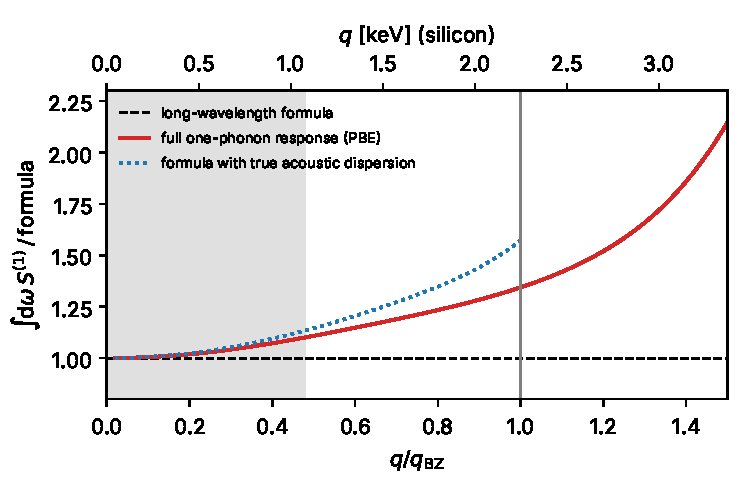
\includegraphics[width=\linewidth]{figures/ch11/limit11_1a.pdf}
\captionof{figure}{The $\omega$-integrated one-phonon response of silicon at $T = 0$, \cref{eq:11.1-S1} with all six branches, Umklapp terms and the Debye--Waller factor (solid), divided by the long-wavelength form \cref{eq:11.1-Sac} (dashed, one), both averaged over the directions of $\vect{q}$, against $q/q_{\mathrm{BZ}}$, with $q_{\mathrm{BZ}} = \SI{2.25}{keV}$. Phonons from the PBE force constants of \cref{sec:5.2}, Fourier-interpolated; the formula uses the sound speeds and polarizations of the same force constants, so that the ratio tends to one as $q \to 0$. Dotted: the long-wavelength polarizations with the true acoustic dispersion $\omega_{\vect{q}\nu}$ in place of $c_\nu q$, the leading correction. Gray: $q < 0.48\,q_{\mathrm{BZ}} = \SI{1.08}{keV}$, where the full response and the long-wavelength form agree within \SI{10}{\percent}; they agree within \SI{5}{\percent} below $0.34\,q_{\mathrm{BZ}}$. At $q_{\mathrm{BZ}}$ the formula is \SI{26}{\percent} low.}\label{fig:11-limit-a}
\par}
\smallskip
Toward the zone boundary the acoustic branches bend below $c_\nu q$, and since the weight goes as $1/\omega$, the long-wavelength form underestimates the response; beyond $q_{\mathrm{BZ}}$ the phonon carries only the reduced momentum, and the response grows as $q^2$, the incoherent form of \cref{sec:11.3}.
\end{limitbox}

The dispersion accounts for most of the departure of the full response from \cref{eq:11.1-Sac} below $q_{\mathrm{BZ}}/2$; the polarizations and the phases $\ee^{\ii\vect{q}\cdot\vect{\tau}_\kappa}$ change the ratio at order $(qa)^2$ with the opposite sign. For a rate weighted toward small $q$, as with a light mediator, the region below $q_{\mathrm{BZ}}/2$ gives nearly all of the rate and the formula is accurate. For a heavy mediator the rate is weighted toward the largest $q$ that kinematics allows, $2\mchi v_{\mathrm{max}}$, and the response there stays within \SI{10}{\percent} of the formula only for masses up to about $0.48\,q_{\mathrm{BZ}}/2v_{\mathrm{max}} = \SI{0.20}{MeV}$ in silicon.

\subsection{Orientation-averaged rate}

A crystal at a fixed orientation sees the dark-matter wind from one direction, and its rate depends on that direction; this dependence is the daily modulation of \cref{sec:11.7}. For a rate averaged over the orientations of the crystal, the response enters through its average over the directions of $\vect{q}$, and the velocity integral of \cref{eq:8.2-spectrum} acts on the delta function alone. The velocity integral gives $\eta(\vmin)/2q$ per unit $\dd^3q/(2\pi)^3$, with $\eta$ the mean inverse speed of \cref{eq:1.3-eta} (\cref{sec:8.2}). For a phonon of energy $\omega = c_\nu q$ and elastic scattering, \cref{eq:1.3-vmin} gives
\begin{equation*}
  \vmin = c_\nu + \frac{q}{2\mchi} ,
\end{equation*}
the sound speed plus half the speed the dark matter loses. We write the potential as in \cref{sec:1.4}, $|\tilde V_N(q)|^2 = \pi\sigma_p\FDM(q)^2/\mu_{\chi p}^2$, with $\sigma_p$ the dark-matter--proton cross-section, $\mu_{\chi p}$ the reduced mass and $\FDM$ the form factor of \cref{eq:1.4-defs} with $q_0 = \alpha m_e$. Inserting \cref{eq:11.1-Sac} into \cref{eq:8.2-spectrum}, integrating $\omega$ above a threshold $\omega_{\mathrm{th}}$ and collecting $4\pi\cdot\pi\cdot\pi/(2(2\pi)^3) = 1/4$ gives
\begin{keyresult}[One-acoustic-phonon rate per unit mass]
\begin{equation}
  \mathcal{R} = \frac{\rho_\chi\,\sigma_p}{4\,\mchi\,\mu_{\chi p}^2\,m_u^2}\,\Bigl\langle\sum_{\nu = 1}^{3}\frac{(\hat{\vect{q}}\cdot\hat{\vect{e}}_\nu)^2}{c_\nu}\int_{\omega_{\mathrm{th}}/c_\nu}^{q_{\mathrm{up},\nu}}\dd q\;q^2\,\FDM(q)^2\,\eta\Bigl(c_\nu + \frac{q}{2\mchi}\Bigr)\Bigr\rangle_{\hat{\vect{q}}} ,
  \label{eq:11.1-rate}
\end{equation}
with $c_\nu$ and $\hat{\vect{e}}_\nu$ taken at $\hat{\vect{q}}$, the brackets the average over the sphere of directions, and the upper limit $q_{\mathrm{up},\nu} = \min[2\mchi(v_{\mathrm{max}} - c_\nu),\,q_{\mathrm{BZ}}]$.
\end{keyresult}
\noindent The kinematic upper limit is where $\eta$ vanishes, $\vmin = v_{\mathrm{max}}$; the zone cut $q_{\mathrm{BZ}}$ is the range of \cref{eq:11.1-Sac}, beyond which the multiphonon response of \cref{sec:11.3} dominates. The rate is nonzero only when the lower limit lies below the upper one, $\omega_{\mathrm{th}}/c_\nu \le 2\mchi(v_{\mathrm{max}} - c_\nu)$, and this condition defines the \emph{acoustic edge} of \cref{sec:9.2},
\begin{equation}
  m_{\mathrm{min}}^{\mathrm{ac}} = \frac{\omega_{\mathrm{th}}}{2c_\nu(v_{\mathrm{max}} - c_\nu)} \simeq \frac{\omega_{\mathrm{th}}}{2c_\nu v_{\mathrm{max}}} ,
  \label{eq:11.1-edge}
\end{equation}
set by the largest speed of a branch with longitudinal weight over all directions, $c_{\mathrm{LA,max}}$. For silicon at $\omega_{\mathrm{th}} = \SI{1}{meV}$, $c_{\mathrm{LA,max}} = \SI{9.35}{km.s^{-1}}$ along $[111]$ and $m_{\mathrm{min}}^{\mathrm{ac}} = \SI{6.1}{keV}$, against \SI{0.28}{keV} for the threshold mass.

\begin{figure}[tbp]
  \centering
  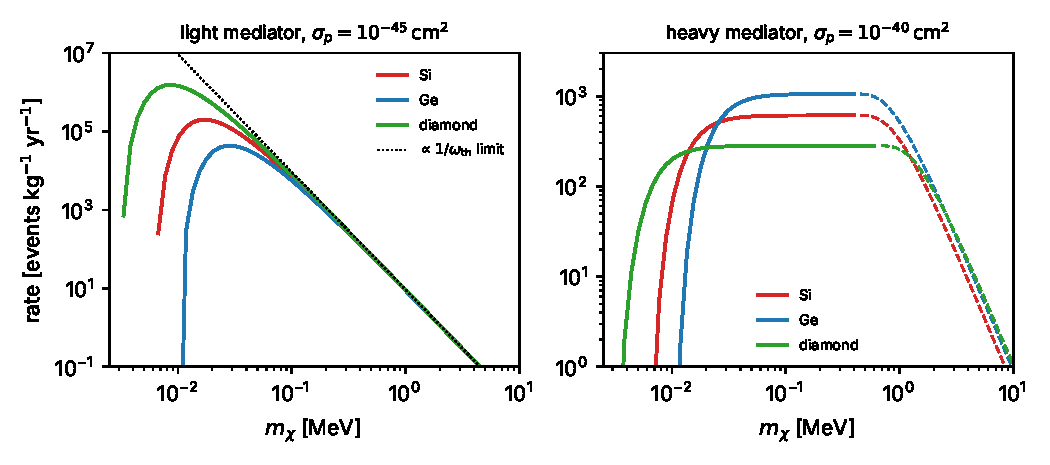
\includegraphics[width=\linewidth]{figures/ch11/fig11_1.pdf}
  \caption{Rate of single-acoustic-phonon emission per unit target mass, \cref{eq:11.1-rate}, for silicon, germanium and diamond at a threshold $\omega_{\mathrm{th}} = \SI{1}{meV}$, averaged over the orientation of the crystal, with equal couplings to protons and neutrons, $\rho_\chi = \SI{0.3}{GeV.cm^{-3}}$ and the standard halo of \cref{sec:1.2}. Sound speeds and polarizations from the Christoffel problem of the measured room-temperature elastic tensors (\cref{we:11-cbar}); momentum transfers $q \le q_{\mathrm{BZ}}$, Debye--Waller factor one. Left: light mediator, $\FDM = (q_0/q)^2$, $\sigma_p = 10^{-45}\,\mathrm{cm^2}$; dotted, the target-independent limit \cref{eq:11.1-light}. Right: heavy mediator, $\FDM = 1$, $\sigma_p = 10^{-40}\,\mathrm{cm^2}$; solid up to $q_{\mathrm{BZ}}/2v_{\mathrm{max}}$ (0.42, 0.41 and \SI{0.65}{MeV}), dashed above, where the fall is an artifact of the cut $q \le q_{\mathrm{BZ}}$ and where the multiphonon and Umklapp terms of \cref{sec:11.3} dominate. The edges are 6.1 (Si), 10.2 (Ge) and \SI{3.1}{keV} (diamond).}
  \label{fig:11-rate}
\end{figure}

\subsection{Light mediator}

For a light mediator, $\FDM^2 = (q_0/q)^4$, the integrand of \cref{eq:11.1-rate} falls as $q^{-2}$, and the rate is dominated by the smallest momentum transfer that a phonon above threshold can carry. In the variable $u = q/2\mchi$, the integral of one branch and direction is
\begin{equation*}
  \frac{q_0^4}{2\mchi}\int_{u_-}^{u_+}\dd u\,\frac{\eta(c_\nu + u)}{u^2} , \qquad u_- = \frac{\omega_{\mathrm{th}}}{2\mchi c_\nu} , \quad u_+ = v_{\mathrm{max}} - c_\nu .
\end{equation*}
Far above the edge, where $u_- \ll u_+$, the integral tends to $\eta(c_\nu)/u_-$, and since $u_- = \omega_{\mathrm{th}}/2\mchi c_\nu$, the $q$-integral of each branch and direction is $q_0^4c_\nu\eta(c_\nu)/\omega_{\mathrm{th}}$. Its factor $c_\nu$ cancels the weight $1/c_\nu$ in the brackets of \cref{eq:11.1-rate}. The shift of $\eta$ by $c_\nu$ is of relative order $c_\nu^2/v_0^2 \sim 10^{-3}$, since the laboratory speed distribution vanishes as $v^2$ at small speeds and $\eta$ is flat at the origin. By the completeness $\sum_\nu(\hat{\vect{q}}\cdot\hat{\vect{e}}_\nu)^2 = 1$ the weights of the directions and branches then add up to one, and
\begin{equation}
  \mathcal{R}_{\mathrm{light}} = \frac{\rho_\chi\,\sigma_p\,q_0^4\,\eta(0)}{4\,\mchi\,\mu_{\chi p}^2\,m_u^2\,\omega_{\mathrm{th}}} .
  \label{eq:11.1-light}
\end{equation}
The rate per unit mass is the same for every crystal, inversely proportional to the threshold, and it falls as $\mchi^{-3}$ for $\mchi \ll m_p$. The light-mediator curves of \cref{fig:11-rate} merge with \cref{eq:11.1-light} at high mass. They separate near the edges, which differ by a factor of three between diamond and germanium.

To find how far above the edge the limit \cref{eq:11.1-light} holds, write $\eta(c_\nu + u) = \eta(0) - [\eta(0) - \eta(c_\nu + u)]$. The first term integrates to $\eta(0)(1/u_- - 1/u_+)$. In the second term, the bracket vanishes as $u^2$ at small $u$, so the integral of the second term from $0$ to $u_-$ is of order $u_-$, and to first order in $u_-$ this integral can run from $0$ to $u_+$. We define
\begin{equation}
  \kappa_\eta = \frac{u_+}{\eta(0)}\int_0^{u_+}\dd u\,\frac{\eta(0) - \eta(u)}{u^2} ,
  \label{eq:11.1-kappa}
\end{equation}
and use $u_-/u_+ = m_{\mathrm{min}}^{\mathrm{ac}}/\mchi$ from \cref{eq:11.1-edge}. The integral of one branch and direction is then $(\eta(0)/u_-)[1 - (1 + \kappa_\eta)\,m_{\mathrm{min}}^{\mathrm{ac}}/\mchi]$ up to terms of second order in $m_{\mathrm{min}}^{\mathrm{ac}}/\mchi$. The rate is therefore
\begin{equation}
  \frac{\mathcal{R}}{\mathcal{R}_{\mathrm{light}}} = \Bigl[1 - (1 + \kappa_\eta)\frac{m_{\mathrm{min}}^{\mathrm{ac}}}{\mchi} + O\Bigl(\frac{m_{\mathrm{min}}^{\mathrm{ac}}}{\mchi}\Bigr)^{\!2}\Bigr] , \qquad \kappa_\eta = 3.14 ,
  \label{eq:11.1-correction}
\end{equation}
with $\mathcal{R}_{\mathrm{light}}$ the limit \cref{eq:11.1-light}, for $\mchi \le q_{\mathrm{BZ}}/2v_{\mathrm{max}}$, where the kinematic limit $u_+$ applies. The value of $\kappa_\eta$ is a property of the halo alone: it is \cref{eq:11.1-kappa} for the standard halo of \cref{sec:1.2} with $u_+ = v_{\mathrm{max}}$, the limit $c_\nu \ll v_{\mathrm{max}}$. At the sound speed of silicon, $u_+ = v_{\mathrm{max}} - c_\nu$ and $\kappa_\eta = 3.09$. The material enters only through the edge, and the term $1$ of $1 + \kappa_\eta$ is the loss of the momentum transfers above $u_+$, and the term $\kappa_\eta$ is the loss of the slow particles that the halo lacks. For a crystal the edge in \cref{eq:11.1-correction} is the average over directions and branches, weighted like the rate: this average equals $m_{\mathrm{min}}^{\mathrm{ac}}$ evaluated at the speed $\langle\sum_\nu(\hat{\vect{q}}\cdot\hat{\vect{e}}_\nu)^2/c_\nu\rangle^{-1}$, and for silicon the speed is \SI{8.956}{km.s^{-1}} (\cref{we:11-cbar}) and the edge \SI{6.39}{keV}. Above $q_{\mathrm{BZ}}/2v_{\mathrm{max}}$ the zone cut replaces $u_+$, and the bracket tends to $1 - \omega_{\mathrm{th}}/(c_\nu q_{\mathrm{BZ}})$, 0.985 for silicon at \SI{1}{meV}.

\begin{limitbox}[Light-mediator single-phonon rate][lim:11.1b]
For a light mediator the one-phonon rate per unit target mass is $\mathcal{R} = \rho_\chi\sigma_pq_0^4\eta(0)/(4\mchi\mu_{\chi p}^2m_u^2\omega_{\mathrm{th}})$, inversely proportional to the threshold and independent of the target~\cite[Eq.~(35)]{griffin2020multichannel}.
\par\smallskip
{\centering
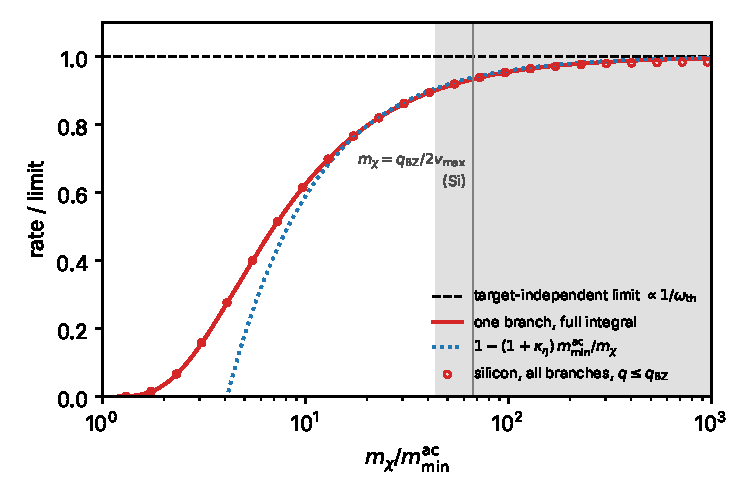
\includegraphics[width=\linewidth]{figures/ch11/limit11_1b.pdf}
\captionof{figure}{The light-mediator rate \cref{eq:11.1-rate}, divided by its target-independent limit \cref{eq:11.1-light} (dashed, one), against $\mchi/m_{\mathrm{min}}^{\mathrm{ac}}$. Solid: one branch of speed \SI{9.0}{km.s^{-1}} without the zone cut; the curve changes by \SI{3}{\percent} at $\mchi = 10\,m_{\mathrm{min}}^{\mathrm{ac}}$ between speeds of 3 and \SI{18}{km.s^{-1}}. Circles: silicon, all branches and directions, with $q \le q_{\mathrm{BZ}}$; on this axis $m_{\mathrm{min}}^{\mathrm{ac}} = \SI{6.39}{keV}$ at $\omega_{\mathrm{th}} = \SI{1}{meV}$, the edge for the polarization-weighted inverse speed \SI{8.956}{km.s^{-1}} of \cref{eq:11.1-heavy}; the vertical line marks $q_{\mathrm{BZ}}/2v_{\mathrm{max}}$, above which the zone cut holds the ratio at 0.985. Dotted: the first-order correction \cref{eq:11.1-correction} with $\kappa_\eta = 3.09$. Gray: $\mchi \ge 44\,m_{\mathrm{min}}^{\mathrm{ac}}$, where the rate is within \SI{10}{\percent} of the limit. The first-order form is within \SI{10}{\percent} of the full rate for $\mchi \ge 9\,m_{\mathrm{min}}^{\mathrm{ac}}$. Standard halo of \cref{sec:1.2}.}\label{fig:11-limit-b}
\par}
\smallskip
Within a few times the edge the momentum window $[\omega_{\mathrm{th}}/c_\nu,\,2\mchi v_{\mathrm{max}}]$ closes and only the fastest particles of the halo contribute, so the rate falls far below the limit and depends on the material through its edge.
\end{limitbox}

\begin{workedexample}{The light-mediator correction at three times the edge}\label{we:11-light}
Take silicon at $\omega_{\mathrm{th}} = \SI{1}{meV}$, where $m_{\mathrm{min}}^{\mathrm{ac}} = \SI{6.39}{keV}$ for the polarization-weighted inverse speed \SI{8.956}{km.s^{-1}} of \cref{eq:11.1-heavy}, and $\mchi = 3\,m_{\mathrm{min}}^{\mathrm{ac}} = \SI{19.2}{keV}$. The momentum transfers that can create a phonon above threshold run from $\omega_{\mathrm{th}}/c = \SI{33}{eV}$ to $2\mchi(v_{\mathrm{max}} - c) = \SI{100}{eV}$, a factor of three. With $\kappa_\eta = 3.09$ at this sound speed, the first-order factor is $1 - 4.09/3 = -0.36$: negative, and therefore meaningless. The full integral of \cref{eq:11.1-rate}, with all branches and directions, gives $\mathcal{R}/\mathcal{R}_{\mathrm{light}} = 0.149$. The expansion behind \cref{eq:11.1-correction} has failed at this mass, because the speeds that contribute, $\vmin$ between $c + u_-$ and $v_{\mathrm{max}}$, all lie in the tail of the halo above \SI{270}{km.s^{-1}}, where $\eta$ is far from flat. At ten times the edge, \SI{63.9}{keV}, the full ratio is 0.625 and the first-order form 0.591; at 44 times, \SI{0.28}{MeV}, the full ratio is 0.902 and the first-order form 0.907. The target-independent statement holds within \SI{10}{\percent} only from about \SI{0.28}{MeV} in silicon, and for any two materials only above 44 times the higher of their edges.
\end{workedexample}

\subsection{Heavy mediator}

For a heavy mediator, $\FDM = 1$, the integrand of \cref{eq:11.1-rate} grows as $q^2$, and the rate is dominated by the largest momentum transfer, $2\mchi(v_{\mathrm{max}} - c_\nu)$. With $u = q/2\mchi$ the integral of one branch is $8\mchi^3\int_{u_-}^{u_+}\dd u\,u^2\eta(c_\nu + u)$. Well above the edge and with $c_\nu \ll v_{\mathrm{max}}$, it tends to $8\mchi^3I_0$, with $I_0 = \int_0^{v_{\mathrm{max}}}\dd u\,u^2\eta(u) = 5.32\times10^{-7}$ for the standard halo. For $\mchi \ll m_p$ the reduced mass is $\mu_{\chi p} \approx \mchi$, and the factors of $\mchi$ cancel:
\begin{equation}
  \mathcal{R} = \frac{2\rho_\chi\,\sigma_p\,I_0}{m_u^2}\,\Bigl\langle\sum_\nu\frac{(\hat{\vect{q}}\cdot\hat{\vect{e}}_\nu)^2}{c_\nu}\Bigr\rangle_{\hat{\vect{q}}} .
  \label{eq:11.1-heavy}
\end{equation}
The rate per unit mass is independent of the dark-matter mass and inversely proportional to a polarization-weighted mean speed, so soft crystals have the larger rate. The plateaus of \cref{fig:11-rate} nearly stand in the ratio of the inverse speeds, $8.956/5.321 = 1.68$ for germanium against silicon and $8.956/18.16 = 0.49$ for diamond. The computed rates at \SI{0.3}{MeV} stand in the ratios 1.73 and 0.46. The difference between the computed ratios and the ratios of the inverse speeds comes from the shift of $\eta$ by $c_\nu$. The shift matters at the large $u$ that a heavy mediator favors, where $\eta$ is not flat, and lowers the rate of a stiff crystal by several percent per \SI{10}{km.s^{-1}}.

The plateau is reached only well above the edge and, in silicon, ends near \SI{0.42}{MeV}. Near the edge the lower cut removes part of $I_0$, and the rate approaches \cref{eq:11.1-heavy} only slowly, because $\eta$ falls steeply toward $v_{\mathrm{max}}$ and the integrand is weighted toward small $u$. In silicon the rate reaches \SI{90}{\percent} of the plateau value (654 events per kilogram and year at $\sigma_p = 10^{-40}\,\mathrm{cm^2}$) only at \SI{45}{keV}, seven times the edge. However, the silicon rate never exceeds \SI{94}{\percent} of the plateau value, and the diamond rate never exceeds \SI{87}{\percent} of its plateau value, because \cref{eq:11.1-heavy} drops the shift of $\eta$ by $c_\nu$. By \cref{fig:11-limit-a}, from about \SI{0.2}{MeV} the response at the largest momentum transfers already differs from \cref{eq:11.1-Sac} by more than \SI{10}{\percent}. Above $q_{\mathrm{BZ}}/2v_{\mathrm{max}}$, \SI{0.42}{MeV} for silicon, the momentum transfers leave the region where \cref{eq:11.1-Sac} holds, and Umklapp processes and multiphonons dominate (\cref{sec:11.3}). \Cref{sec:17.5} names the inverse of the bracket in \cref{eq:11.1-heavy} the effective sound speed of the channel and ranks materials by it.

\subsection{Sound speeds from the elastic tensor}

The rates above need the sound speeds in every direction, and with them two averages: the largest longitudinal speed for the edge and the polarization-weighted inverse speed of \cref{eq:11.1-heavy}. The speeds and both averages follow from the elastic tensor $C_{ijkl}$ and the density through the Christoffel equation \cref{eq:C.18-christoffel}: in each direction $\hat{\vect{q}}$ the eigenvalues of $\mathsf{M}_{ik} = C_{ijkl}\hat q_j\hat q_l$ are $\rho_Tc_\nu(\hat{\vect{q}})^2$, and the eigenvectors are the polarizations $\hat{\vect{e}}_\nu$ of \cref{eq:11.1-Sac}.

The elastic constants are measured or computed by density-functional theory (\cref{app:E.4}), and a computed tensor must be in the Voigt order of \cref{app:C.18} before it enters the Christoffel matrix.

\begin{workedexample}{The rate coefficient of silicon}\label{we:11-cbar}
The room-temperature constants of silicon are $C_{11} = 165.6$, $C_{12} = 63.9$ and $C_{44} = \SI{79.5}{GPa}$, with $\rho_T = \SI{2.33}{g.cm^{-3}}$ (\cref{app:C.18}). Along the three symmetry directions \cref{eq:C.18-cubic} gives $\rho_Tc_{\mathrm{LA}}^2 = 165.6$, $194.3$ and \SI{203.8}{GPa}, and $c_{\mathrm{LA}} = 8.43$, 9.13 and \SI{9.35}{km.s^{-1}} along $[100]$, $[110]$ and $[111]$. The speed varies by \SI{11}{\percent} over the sphere, and the averages need all directions.

The polarization-weighted average is a quadrature. On a product grid of Gauss--Legendre nodes in $\cos\theta$ and equally spaced nodes in $\phi$ (\cref{app:C.18}), with the $3\times3$ Christoffel matrix diagonalized at each node, the inverse of the rate coefficient of \cref{eq:11.1-heavy}, $\langle\sum_\nu(\hat{\vect{q}}\cdot\hat{\vect{e}}_\nu)^2/c_\nu\rangle^{-1}$, is \SI{8.956}{km.s^{-1}}. The same procedure yields \SI{5.321}{km.s^{-1}} for germanium and \SI{18.16}{km.s^{-1}} for diamond, from the tensors $131$, $49$, \SI{68}{GPa}~\cite{mcskimin1963elastic} and $1081$, $125$, \SI{579}{GPa}~\cite{mcskimin1972elastic}, as tabulated in Ref.~\cite[Table~III]{haxhijaj2026lattice}, with the densities 5.33 and \SI{3.52}{g.cm^{-3}} that follow from the lattice constants 5.658 and \SI{3.567}{\angstrom}.
\end{workedexample}

A tabulated speed can be tested without the full tensor. The largest eigenvalue of the Christoffel matrix is at least its expectation value in the unit vector $\hat{\vect{q}}$. For cubic symmetry that expectation value is never below the bulk modulus $B = (C_{11} + 2C_{12})/3$ of \cref{eq:C.18-bulk}, and the two inequalities give \cref{eq:C.18-rayleigh}:
\begin{equation}
  c_{\mathrm{LA}}(\hat{\vect{q}}) \ge \sqrt{B/\rho_T} \qquad\text{(cubic crystals, every direction)} .
  \label{eq:11.1-rayleigh}
\end{equation}
The bound is \SI{6.48}{km.s^{-1}} for silicon, \SI{3.79}{km.s^{-1}} for germanium and \SI{11.23}{km.s^{-1}} for diamond, 23, 24 and \SI{36}{\percent} below their slowest longitudinal speeds. It is proved for cubic crystals only; for lower symmetries the uniform compression and the uniform strain no longer coincide (\cref{app:C.18}), and the bound must be replaced by the Christoffel eigenvalue itself. \Cref{sec:17.5} applies the bound to tabulated speeds.


\section{Optical phonons in polar crystals}\label{sec:11.2}

A dark-matter particle of \SI{100}{keV} that scatters in GaAs through a light dark photon most often leaves behind one longitudinal optical phonon of \SI{36.35}{meV}. The dark photon does not couple to the nucleons. It couples to the charge, and when the gallium and arsenic sublattices move against each other every cell carries the dipole of their Born charges (\cref{sec:5.5}), whose field the electrons screen. In the acoustic waves of \cref{sec:11.1} the cell moves as a whole and stays neutral, and at long wavelength a coupling to charge has no vertex there; in the optical branch of GaAs its vertex is $Z^*/\varepsilon_\infty = 0.19$ per cell at every small momentum transfer (\cref{we:8-nucleon}). Silicon and germanium, whose Born charges vanish, have no such channel. A polar target enters the rate through one band integral of its loss function, and the crystals with the largest band integrals have the highest kinematic edges.

\subsection{The phonon loss function}\label{sec:11.2-loss}

A dark photon, heavy or light, couples to the charge-number density $n_Z$, and so does any particle with a small electric charge (\cref{we:8-darkphoton}). For this row \cref{sec:8.4} gave an exact answer: $S_{ZZ} = (2q^2/e^2)\,L/(1 - \ee^{-\beta\omega})$, with $L = \Imag[-(\varepsilon^{-1})_{00}]$ the loss function of the total dielectric matrix of electrons and nuclei. Below the band gap the electrons add a constant to $\varepsilon$, and every structure of $L$ there comes from the ions. We need $\varepsilon$ at the frequencies of the optical phonons and at momentum transfers small compared with the zone, where the long-range Coulomb line is the macroscopic field and the rank-one form \cref{eq:8.4-rank1} holds.

The dielectric function along $\hat{\vect{q}}$ follows from the energy \cref{eq:5.5-U}. The electrons follow adiabatically and contribute $\varepsilon_\infty(\hat{\vect{q}}) \equiv \hat{\vect{q}}\cdot\varepsilon_\infty\cdot\hat{\vect{q}}$. The ions respond as the oscillators of the analytic zone-center problem, the eigenmodes of $D^{\mathrm{an}}_{\kappa\kappa'} = C^{\mathrm{an}}_{\kappa\kappa'}/(M_\kappa M_{\kappa'})^{1/2}$ with real polarization vectors and frequencies $\omega_{\mathrm{T}\nu}$, each driven by the field through its mode charge (\cref{eq:5.5-HE}). Collecting the $3n$ components of the $n$ sublattices into one vector,
\begin{equation}
  \varepsilon(\hat{\vect{q}},\omega) = \varepsilon_\infty(\hat{\vect{q}}) + \frac{e^2}{\Omega}\,\vect{p}^{\mathrm{T}}\bigl(D^{\mathrm{an}} - \omega^2\bigr)^{-1}\vect{p} ,
  \qquad p_{\kappa\alpha}(\hat{\vect{q}}) = \frac{(Z^*_\kappa\cdot\hat{\vect{q}})^\alpha}{\sqrt{M_\kappa}} ,
  \label{eq:11.2-eps}
\end{equation}
which is \cref{eq:5.5-eps} for any number of atoms and any direction. Expanded in the eigenmodes of $D^{\mathrm{an}}$, the second term is a sum of poles at the transverse frequencies, each weighted by the square of the mode charge along $\hat{\vect{q}}$.

The loss function needs $1/\varepsilon$, and the structure of \cref{eq:11.2-eps} makes the inversion exact. The ionic term is a matrix element of the inverse of $A = D^{\mathrm{an}} - \omega^2$ between one vector, and the Sherman--Morrison identity, $(A + \vect{b}\vect{b}^{\mathrm{T}})^{-1} = A^{-1} - A^{-1}\vect{b}\vect{b}^{\mathrm{T}}A^{-1}/(1 + \vect{b}^{\mathrm{T}}A^{-1}\vect{b})$, gives $\vect{b}^{\mathrm{T}}(A + \vect{b}\vect{b}^{\mathrm{T}})^{-1}\vect{b} = \vect{b}^{\mathrm{T}}A^{-1}\vect{b}/(1 + \vect{b}^{\mathrm{T}}A^{-1}\vect{b})$. With $\vect{b} = e\vect{p}/[\Omega\varepsilon_\infty(\hat{\vect{q}})]^{1/2}$, \cref{eq:11.2-eps} reads $\varepsilon = \varepsilon_\infty(\hat{\vect{q}})(1 + \vect{b}^{\mathrm{T}}A^{-1}\vect{b})$, and therefore
\begin{equation}
  \frac{1}{\varepsilon(\hat{\vect{q}},\omega)} = \frac{1}{\varepsilon_\infty(\hat{\vect{q}})}\Bigl[1 - \vect{b}^{\mathrm{T}}\bigl(D^{\mathrm{an}} + \vect{b}\vect{b}^{\mathrm{T}} - \omega^2\bigr)^{-1}\vect{b}\Bigr] .
  \label{eq:11.2-SM}
\end{equation}
The matrix $D^{\mathrm{an}} + \vect{b}\vect{b}^{\mathrm{T}}$ is the dynamical matrix \cref{eq:5.5-na}: $\vect{b}\vect{b}^{\mathrm{T}}$ is exactly its nonanalytic term. Inverting $\varepsilon$ has traded the poles of $\varepsilon$, at the transverse frequencies, for the eigenfrequencies of the full dynamical matrix, which include the longitudinal ones. Let $\omega_\nu$ and $\vect{e}_\nu$ be its eigenpairs for the direction $\hat{\vect{q}}$. Then $\vect{b}^{\mathrm{T}}(D^{\mathrm{dyn}} - \omega^2)^{-1}\vect{b} = \sum_\nu(\vect{b}\cdot\vect{e}_\nu)^2/(\omega_\nu^2 - \omega^2)$, and with $\omega \to \omega + \ii0^+$ each term has the imaginary part $\pi(\vect{b}\cdot\vect{e}_\nu)^2\,\delta(\omega - \omega_\nu)/2\omega_\nu$ for $\omega > 0$. The loss function in the phonon band is a set of lines,
\begin{equation*}
  L(\hat{\vect{q}},\omega) = \frac{\pi e^2}{2\Omega\,\varepsilon_\infty(\hat{\vect{q}})^2}\sum_\nu\frac{(\vect{p}\cdot\vect{e}_\nu)^2}{\omega_\nu}\,\delta(\omega - \omega_\nu) .
\end{equation*}
Of these steps only the vertex needs $\vect{q} = 0$. At a wavevector inside the zone, $D^{\mathrm{an}}$ becomes the dynamical matrix at $\vect{Q}$ with the macroscopic field removed, each component of $\vect{p}$ takes the phase $\ee^{\ii\vect{q}\cdot\vect{\tau}_\kappa}$ of its site, and $D^{\mathrm{an}} + \vect{b}\vect{b}^{\mathrm{T}}$ is the full dynamical matrix at $\vect{Q}$. Multiplying by $2q^2/e^2$:
\begin{keyresult}[Born-charge one-phonon structure factor]
\begin{equation}
  S^{(1)}_{ZZ}(\vect{q},\omega) = \frac{2\pi}{\Omega}\sum_\nu\frac{\bigl|\sum_\kappa\ee^{\ii\vect{q}\cdot\vect{\tau}_\kappa}\,\vect{e}_{\kappa\nu}(\vect{Q})^*\cdot Z^*_\kappa\cdot\vect{q}/\sqrt{M_\kappa}\bigr|^2}{2\omega_{\vect{Q}\nu}\,\bigl(\hat{\vect{q}}\cdot\varepsilon_\infty\cdot\hat{\vect{q}}\bigr)^2}\,\delta(\omega - \omega_{\vect{Q}\nu}) ,
  \label{eq:11.2-SZZ}
\end{equation}
at $T = 0$, for $q$ small compared with the zone and $\omega$ far below the gap, with the phonons of the full dynamical matrix, nonanalytic term included, and the phase convention of \cref{eq:11.1-S1}.
\end{keyresult}
\noindent The structure is that of the nucleon response \cref{eq:11.1-S1}, with the nucleon number $A_\kappa$ replaced by the Born charge projected on $\vect{q}$ and the whole vertex divided by $\varepsilon_\infty(\hat{\vect{q}})$. Each branch contributes the square of its dipole along $\vect{q}$, screened by the electrons, divided by its energy. At the zone center the acoustic branches drop out by the neutrality \cref{eq:5.5-neutral}, and in a cubic crystal so do the transverse optical ones, whose dipole is perpendicular to $\vect{q}$. The longitudinal mode, at $\omega_{\mathrm{L}}$, remains. The proper response of the ions has its poles at $\omega_{\mathrm{T}}$, but the transverse pole of $\varepsilon$ is a zero of $1/\varepsilon$, and a coupling to charge excites the longitudinal phonon, as in absorption (\cref{sec:5.5}).

The loss function of the total $\varepsilon$ and the Born-charge vertex screened by $\varepsilon_\infty$ are two resummations of the series \cref{eq:8.4-screened}, one with the ions inside the dielectric function and one with them in the vertex, and \cref{eq:11.2-SM} is the step between them. The vertex is that of \cref{sec:6.2}, the Fr\"ohlich vertex \cref{eq:D.14-gL} with the electron replaced by the dark particle: the density vertex $\rho_{mn}$ becomes one, and the charge of the electron becomes the coupling of the dark matter.

Every input of \cref{eq:11.2-SZZ} is an output of density-functional perturbation theory: phonons at $\vect{Q}$ with the nonanalytic term, Born charges and $\varepsilon_\infty$ (\cref{app:E.4}). The rate carries $(Z^*/\varepsilon_\infty)^2$, and the semilocal $\varepsilon_\infty$ of GaAs, \SI{26}{\percent} too high (\cref{sec:5.5}), would make it \SI{37}{\percent} too low. We use instead the computed phonons and Born charge with the measured room-temperature $\varepsilon_\infty = 10.88$ and $\varepsilon_0 = 12.9$ of GaAs~\cite{lockwood2005optical}, or the measured splitting itself (\cref{sec:11.2-split}).

\Cref{eq:11.2-SZZ} holds when the momentum transfer is small compared with the zone, the energy far below the gap, and the lattice harmonic and cold. At small momentum transfer the charge that moves with a nucleus is its Born charge; corrections to this vertex start at relative order $qa$. Far below the gap the electrons follow the ions adiabatically and the vertex may be computed at zero frequency; by the argument of \cref{sec:8.4} the error is of order $(\omega_{\mathrm{L}}/\Eg)^2$, $6\times10^{-4}$ in GaAs. For the cold harmonic lattice, the Debye--Waller factor is $1 - 8\times10^{-8}$ at the smallest momentum transfer, $q = \omega_{\mathrm{L}}/v_{\mathrm{max}} = \SI{13.7}{eV}$, with the root-mean-square displacement of \cref{tab:5-phonons}. At \SI{10}{mK}, $\omega_{\mathrm{L}}/T = 4.2\times10^4$ and no optical phonon is thermally occupied. The anharmonic width of the longitudinal phonon, a fraction of a meV, spreads the line without moving its weight. The small-$q$ vertex is the condition that matters in practice, and the limit check tests it with the phonons of \cref{fig:5-gaas}.

\begin{limitbox}[Born-charge single-phonon rate][lim:11.2a]
A particle that couples to charge creates one phonon with the structure factor \cref{eq:11.2-SZZ}: Born charges, screened by $\varepsilon_\infty$, acting on the phonons of the full dynamical matrix~\cites[Eqs.~(92), (105), (106)]{trickle2020multichannel}[Eqs.~(19), (23)]{griffin2018directional}[Eq.~(61)]{trickle2022effective}. For one longitudinal branch this is the form of Knapen and collaborators~\cite[Eqs.~(4)--(7)]{knapen2018detection}.
\par\smallskip
{\centering
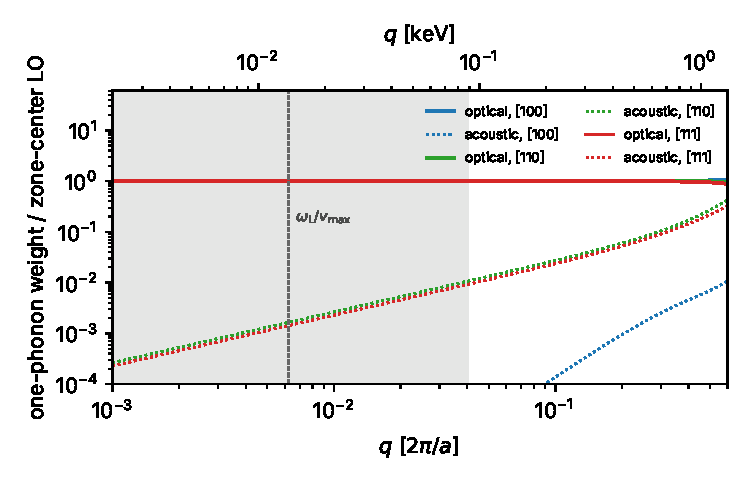
\includegraphics[width=\linewidth]{figures/ch11/limit11_2a.pdf}
\captionof{figure}{One-phonon weight of GaAs in \cref{eq:11.2-SZZ}, $\sum_\nu|\sum_\kappa\ee^{\ii\vect{q}\cdot\vect{\tau}_\kappa}\vect{e}^*_{\kappa\nu}\cdot Z^*_\kappa\cdot\hat{\vect{q}}/\sqrt{M_\kappa}|^2/2\omega_\nu$, divided by its zone-center value $Z^{*2}/2\mu_{\mathrm{red}}\omega_{\mathrm{L}}$, against $q$ along $[100]$, $[110]$ and $[111]$. Solid: the three optical branches; dotted: the three acoustic branches. Phonons at the actual $\vect{q}$ from the PBE force constants of \cref{fig:5-gaas}; Born charges held at their zone-center value. The ratios do not depend on $Z^*$ or $\varepsilon_\infty$. Gray: $q < 0.04 \times 2\pi/a = \SI{88}{eV}$, where the optical weight is within $10^{-4}$ of the formula and the acoustic weight is at most about \SI{1}{\percent}. Dashed line: $q = \omega_{\mathrm{L}}/v_{\mathrm{max}}$, the smallest momentum transfer that reaches the longitudinal phonon.}\label{fig:11-limit-2a}
\par}
\smallskip
At $q$ comparable with $2\pi/a$ the Born charge no longer describes the charge that moves with a nucleus, and the acoustic branches acquire a piezoelectric charge that the Born charges fix only in part.
\end{limitbox}

The optical weight stays within $10^{-4}$ of its zone-center value up to \SI{88}{eV} and within \SI{0.4}{\percent} up to \SI{450}{eV}, where the longitudinal branch has dispersed by \SI{0.3}{meV}. The acoustic branches are the leading correction, and they grow linearly in $q$: their weight reaches \SI{1}{\percent} of the optical one at \SI{90}{eV} along $[111]$ and \SI{5}{\percent} at \SI{450}{eV}, while along $[100]$ it vanishes by symmetry. This is the piezoelectric charge of \cref{sec:6.2}. With rigid Born charges an acoustic wave polarizes the cell only through the relative displacement of the sublattices that its strain induces; the dynamical quadrupoles of the displaced atoms, the next term beyond the Born charge in the expansion of the charge that moves with an atom in powers of $q$, add a contribution of the same order (\cref{app:E.5}), which the limit check does not include. The dotted curves are an estimate of the size of the correction.

The same order-$qa$ structure of the longitudinal mode sets the whole nucleon vertex of \cref{we:8-nucleon}, which vanishes as $q \to 0$; the charge vertex, finite at $q = 0$, is insensitive to it.

\subsection{The polar single-phonon rate}\label{sec:11.2-rate}

The dark matter enters through one potential. A dark photon couples to $-\tilde V n_Z$, with the same $\tilde V$ on electrons and nuclei, and we normalize it as for electron scattering, $|\tilde V|^2 = \pi\sigmae\FDM^2/\mu_{\chi e}^2$ (\cref{eq:1.4-Vsq}), with $\FDM = (q_0/q)^2$ for a light dark photon. We average the structure factor over the directions of $\vect{q}$, so that the halo enters through $\eta(\vmin)$ (\cref{eq:A.8-eta}); the direction dependence that a crystal keeps is the subject of \cref{sec:11.7}. With $S_{ZZ} = (2q^2/e^2)\bar L$ at $T = 0$, the rate \cref{eq:A.8-rateiso} becomes, for the light mediator,
\begin{keyresult}[Polar single-phonon rate]
\begin{equation}
  \mathcal{R} = \frac{\rho_\chi\,\sigmae\,q_0^4}{2\pi\,\mchi\,\mu_{\chi e}^2\,e^2\,\rho_T}\int_{\mathrm{band}}\dd\omega\;\bar L(\omega)\,K_\eta(\omega,\mchi) ,
  \qquad
  K_\eta(\omega,\mchi) = \int\frac{\dd q}{q}\;\eta\bigl(\vmin(q,\omega)\bigr) ,
  \label{eq:11.2-rate}
\end{equation}
with $\bar L$ the loss function at small $q$, averaged over directions, and the integral over the phonon band.
\end{keyresult}
\noindent All powers of $q$ cancel but one. A light mediator weights every logarithmic interval of momentum transfer equally, and the phonon fixes the energy deposited. The rate is then the loss function summed over the band, each line weighted by a kinematic factor that depends only on its energy and the dark-matter mass. Since $\vmin(q,\omega) \ge (2\omega/\mchi)^{1/2}$ at every $q$, the factor vanishes below the mass at which the fastest particle can deposit $\omega$, $2\omega/v_{\mathrm{max}}^2$ (\cref{eq:1.3-mmin}), which is \SI{10.35}{keV} for the longitudinal phonon of GaAs. For a single speed $v$, $\eta = \Theta(v - \vmin)/v$ and $K_\eta = \ln(q_+/q_-)/v$, with $q_\pm = \mchi v[1 \pm (1 - 2\omega/\mchi v^2)^{1/2}]$ the ends of the kinematic window.

For a heavy mediator, $\FDM = 1$, the same steps replace $K_\eta$ by $q_0^{-4}\int\dd q\,q^3\eta$, and the rate is weighted toward the largest momentum transfer, $2\mchi v_{\mathrm{max}}$. It leaves the region of \cref{fig:11-limit-2a}, where the acoustic share stays below a few percent, at about $0.2\times2\pi/a$, or $\mchi \approx \SI{83}{keV}$ in GaAs. The optical phonons alone keep the one-branch form to about \SI{0.1}{\percent} at \SI{99}{keV}; the vertex fails first.

\begin{figure}[tbp]
  \centering
  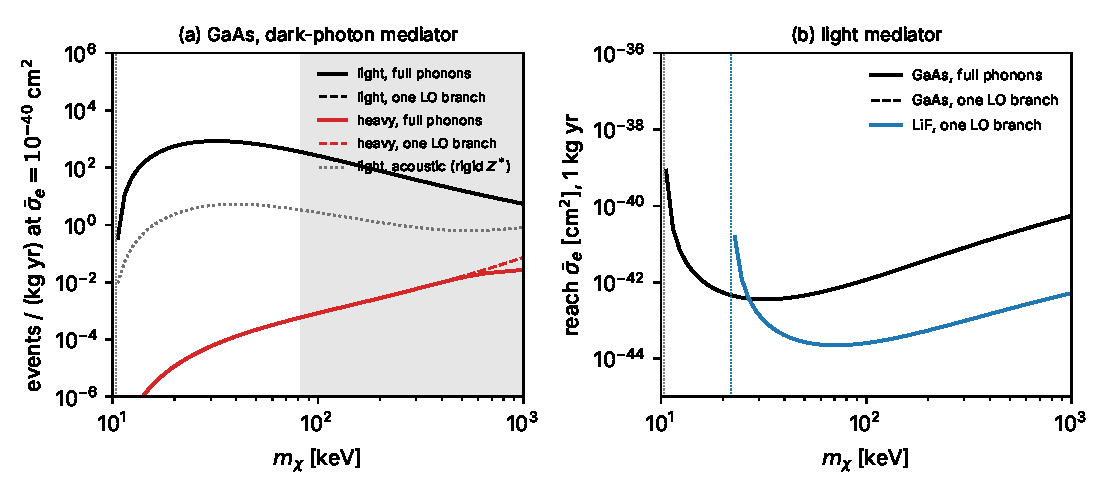
\includegraphics[width=\linewidth]{figures/ch11/fig11_2.pdf}
  \caption{Single-phonon scattering of dark matter through a dark photon in polar crystals, for the standard halo of \cref{sec:1.2} at $T = 0$. (a) Rate of GaAs per kilogram and year at $\sigmae = \SI{e-40}{cm^2}$, light ($\FDM = (q_0/q)^2$) and heavy ($\FDM = 1$) mediator. Solid: \cref{eq:11.2-SZZ} with the three optical branches of the PBE phonons of \cref{fig:5-gaas}, at the actual $\vect{q}$ (Umklapp included), averaged over 146 directions, in \cref{eq:A.8-rateiso}. Dashed: one longitudinal branch at the zone center, \cref{eq:11.2-onebranch} in \cref{eq:11.2-rate}. Both use $Z^* = 2.11$, the measured $\varepsilon_\infty = 10.88$, $\omega_{\mathrm{L}} = \SI{36.34}{meV}$ (DFPT) and $\rho_T = \SI{5.361}{g.cm^{-3}}$. Dotted: the acoustic branches with the same rigid Born charges and a \SI{1}{meV} threshold, an estimate of the piezoelectric correction (\cref{fig:11-limit-2a}). Gray: $2\mchi v_{\mathrm{max}} > 0.2\times2\pi/a$, where the Born-charge vertex is no longer reliable for the heavy mediator. (b) Light-mediator reach, three events in one kilogram-year without background: GaAs as in (a), and LiF with one longitudinal branch and the computed $Z^* = 1.05$, $\varepsilon_\infty = 2.02$ and $\omega_{\mathrm{L}} = \SI{77.2}{meV}$ of Ref.~\cite[Table~I]{griffin2020multichannel}. Vertical lines: the edges $2\omega_{\mathrm{L}}/v_{\mathrm{max}}^2 = 10.35$ and \SI{21.98}{keV}.}
  \label{fig:11-polar}
\end{figure}

\Cref{fig:11-polar}a shows the result for GaAs. The light-mediator rate rises from the edge to about 840 events per kilogram and year near \SI{29}{keV} for $\sigmae = \SI{e-40}{cm^2}$, and falls at larger masses as $\mu_{\chi e}^{-2}\mchi^{-1}$, with a logarithmic rise of $K_\eta$ on top. The full calculation agrees with the one-branch form to $3\times10^{-4}$ below \SI{300}{keV}; at \SI{1}{MeV} it is \SI{4}{\percent} lower, because part of the logarithmic integral then comes from momentum transfers beyond the zone. The acoustic branches, with rigid Born charges and a \SI{1}{meV} threshold, add at most \SI{3}{\percent}, near the edge, and about \SI{1}{\percent} at \SI{100}{keV}.

\subsection{The band integral}\label{sec:11.2-band}

GaAs has one polar branch, and the loss function has one line. By \cref{eq:5.5-eps}, $1/\varepsilon = \varepsilon_\infty^{-1}(\omega_{\mathrm{T}}^2 - \omega^2)/(\omega_{\mathrm{L}}^2 - \omega^2)$, whose pole at $\omega_{\mathrm{L}}$ leads to $L = (\pi\omega_{\mathrm{L}}/2)\varepsilon_\infty^{-1}(1 - \omega_{\mathrm{T}}^2/\omega_{\mathrm{L}}^2)\,\delta(\omega - \omega_{\mathrm{L}})$. By the Lyddane--Sachs--Teller relation the bracket is $1 - \varepsilon_\infty/\varepsilon_0$, and
\begin{equation}
  S_{ZZ}(\vect{q},\omega) = \frac{\pi q^2\omega_{\mathrm{L}}}{e^2}\Bigl(\frac{1}{\varepsilon_\infty} - \frac{1}{\varepsilon_0}\Bigr)\,\delta(\omega - \omega_{\mathrm{L}})
  = \frac{\pi q^2Z^{*2}}{\Omega\,\mu_{\mathrm{red}}\,\varepsilon_\infty^2\,\omega_{\mathrm{L}}}\,\delta(\omega - \omega_{\mathrm{L}}) .
  \label{eq:11.2-onebranch}
\end{equation}
The second form is \cref{eq:11.2-SZZ} with the longitudinal eigenvector of \cref{app:D.14}, $\vect{e}_1 = (M_2/M_{\mathrm{cell}})^{1/2}\hat{\vect{q}}$ and $\vect{e}_2 = -(M_1/M_{\mathrm{cell}})^{1/2}\hat{\vect{q}}$, for which $\sum_\kappa\vect{e}_\kappa\cdot Z^*_\kappa\cdot\vect{q}/\sqrt{M_\kappa} = Z^*q/\sqrt{\mu_{\mathrm{red}}}$; the two forms are equal by \cref{eq:5.5-LOTO,eq:5.5-LST}.

With several polar branches, how is the weight of $L$ shared among them? A sum rule answers part of the question exactly. The inverse-moment relation \cref{eq:4.4-inverse}, a consequence of causality alone, reads $(2/\pi)\int\dd\omega\,L/\omega = 1 - 1/\varepsilon_0$ for the total dielectric function and $1 - 1/\varepsilon_\infty$ with the nuclei clamped. Since the gap separates the two bands, the difference belongs to the phonons:
\begin{equation}
  \frac{2}{\pi}\int_{\mathrm{band}}\dd\omega\;\frac{L(\omega)}{\omega} = \frac{1}{\varepsilon_\infty} - \frac{1}{\varepsilon_0} .
  \label{eq:11.2-kk}
\end{equation}
At small $q$ the band is a set of lines, $L = \sum_\nu(\pi\omega_{\mathrm{L}\nu}/2)\,w^{\mathrm{pol}}_\nu\,\delta(\omega - \omega_{\mathrm{L}\nu})$, with the weights $w^{\mathrm{pol}}_\nu = e^2(\vect{p}\cdot\vect{e}_\nu)^2/(\Omega\varepsilon_\infty^2\omega_{\mathrm{L}\nu}^2)$ read off from the line formula above, and \cref{eq:11.2-kk} says that $\sum_\nu w^{\mathrm{pol}}_\nu = 1/\varepsilon_\infty - 1/\varepsilon_0$. The ionic part of the inverse static screening is shared out among the longitudinal branches. The rate needs the zeroth moment instead, the \emph{band integral}
\begin{equation}
  \begin{gathered}
  \mathcal{I}_{\mathrm{pol}} = \int_{\mathrm{band}}\dd\omega\;L(\omega) = \frac{\pi}{2}\sum_\nu\omega_{\mathrm{L}\nu}\,w^{\mathrm{pol}}_\nu , \\
  \frac{\pi}{2}\Bigl(\frac{1}{\varepsilon_\infty} - \frac{1}{\varepsilon_0}\Bigr)\omega_{\mathrm{L,min}} \le \mathcal{I}_{\mathrm{pol}} \le \frac{\pi}{2}\Bigl(\frac{1}{\varepsilon_\infty} - \frac{1}{\varepsilon_0}\Bigr)\omega_{\mathrm{T,max}}\Bigl(\frac{\varepsilon_0}{\varepsilon_\infty}\Bigr)^{1/2} ,
  \end{gathered}
  \label{eq:11.2-Ipol}
\end{equation}
bracketed by the sum rule. The upper end uses $\omega_{\mathrm{L,max}} \le \omega_{\mathrm{T,max}}(\varepsilon_0/\varepsilon_\infty)^{1/2}$, which holds because every ratio $\omega_{\mathrm{L}\nu}/\omega_{\mathrm{T}\nu}$ exceeds one and their squares multiply to $\varepsilon_0/\varepsilon_\infty$ (\cref{eq:D.14-LSTgen}). It needs only the transverse frequencies and the two dielectric constants.

In a crystal of lower symmetry these statements hold along each principal axis separately. Along a principal axis the lossless $\varepsilon$ of \cref{eq:11.2-eps} rises monotonically between consecutive poles, so that each transverse pole is followed by one longitudinal zero, $\omega_{\mathrm{T}1} < \omega_{\mathrm{L}1} < \omega_{\mathrm{T}2} < \dots$ (\cref{eq:D.14-LSTgen}), and $\varepsilon = \varepsilon_\infty\prod_\nu(\omega_{\mathrm{L}\nu}^2 - \omega^2)/(\omega_{\mathrm{T}\nu}^2 - \omega^2)$. The weights are then the residues of $-1/\varepsilon$ at its zeros, and the $\varepsilon_0$ and $\varepsilon_\infty$ of the sum rule must belong to the same axis and the same model. For a direction off the principal axes the zeros of $\hat{\vect{q}}\cdot\varepsilon\cdot\hat{\vect{q}}$ move with the direction, and the bracket applies axis by axis.

For a diatomic crystal, \cref{eq:11.2-onebranch} gives $\mathcal{I}_{\mathrm{pol}} = (\pi/2)e^2Z^{*2}/(\Omega\mu_{\mathrm{red}}\varepsilon_\infty^2\omega_{\mathrm{L}})$, and per unit mass, with $\rho_T = M_{\mathrm{cell}}/\Omega$,
\begin{equation}
  \frac{\mathcal{I}_{\mathrm{pol}}}{\rho_T} = \frac{\pi}{2}\,\frac{e^2Z^{*2}}{M_{\mathrm{cell}}\,\mu_{\mathrm{red}}\,\varepsilon_\infty^2\,\omega_{\mathrm{L}}} ,
  \label{eq:11.2-diatomic}
\end{equation}
in which the cell volume has dropped out. In general \cref{eq:11.2-rate} is a sum over branches, $\sum_\nu(\pi\omega_{\mathrm{L}\nu}/2)(w^{\mathrm{pol}}_\nu/\rho_T)K_\eta(\omega_{\mathrm{L}\nu},\mchi)$. When $K_\eta$ changes little across the band, it is $\mathcal{I}_{\mathrm{pol}}/\rho_T$ times $K_\eta$ at the weighted mean frequency $\bar\omega_{\mathrm{pol}} = \sum_\nu\omega_{\mathrm{L}\nu}w^{\mathrm{pol}}_\nu/\sum_\nu w^{\mathrm{pol}}_\nu$, and the material enters through $\mathcal{I}_{\mathrm{pol}}/\rho_T$ alone. Sapphire, with four polar branches on its ordinary axis, tests this reading.

\begin{limitbox}[Polar band integral][lim:11.2b]
For one polar branch the light-mediator rate is \cref{eq:11.2-rate} with the line \cref{eq:11.2-onebranch}~\cite[Eqs.~(21), (22), (24)]{griffin2018directional}; with several branches the light-mediator rate per unit mass is proportional to $\mathcal{I}_{\mathrm{pol}}/\rho_T$.
\par\smallskip
{\centering
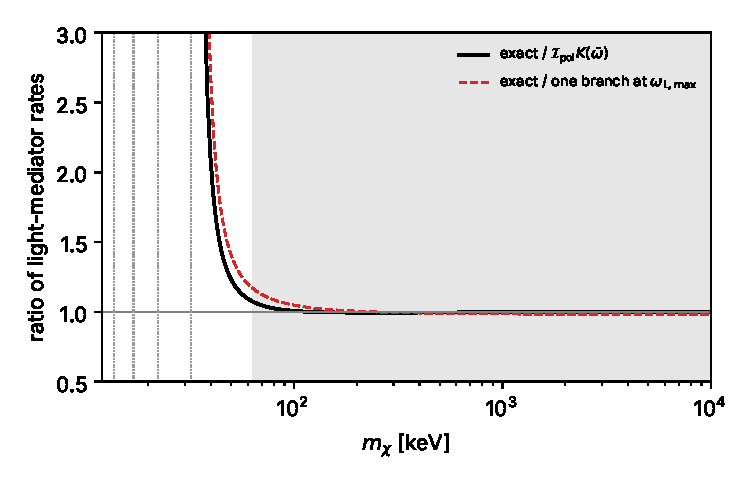
\includegraphics[width=\linewidth]{figures/ch11/limit11_2b.pdf}
\captionof{figure}{Light-mediator rate of the ordinary axis of sapphire, the exact sum over its four longitudinal branches, divided by the band-integral form $\mathcal{I}_{\mathrm{pol}}K_\eta(\bar\omega_{\mathrm{pol}},\mchi)$ (solid) and by the one-branch form with the highest longitudinal frequency and the same $1/\varepsilon_\infty - 1/\varepsilon_0$ (dashed), against $\mchi$. Lossless factorized $\varepsilon$ from the measured frequencies of Ref.~\cite[Table~II]{griffin2018directional} (ordinary ray: longitudinal 112.4, 78.0, 59.7, \SI{48.1}{meV}; transverse 78.6, 70.5, 54.4, \SI{47.7}{meV}) and $\varepsilon_\infty = 3.2$~\cite[Table~I]{griffin2018directional}; weights from the residues of $-1/\varepsilon$, $\bar\omega_{\mathrm{pol}} = \SI{109.9}{meV}$; standard halo of \cref{sec:1.2}. Dotted lines: the four edges $2\omega_{\mathrm{L}\nu}/v_{\mathrm{max}}^2$, from 13.7 to \SI{32.0}{keV}. Gray: $\mchi$ above twice the highest edge, \SI{64}{keV}, where the band-integral form is within \SI{7}{\percent}.}\label{fig:11-limit-2b}
\par}
\smallskip
Within about twice the highest edge the branches open one by one, the lowest first, and the rate follows the individual longitudinal frequencies rather than their weighted sum.
\end{limitbox}

On the ordinary axis of sapphire one branch takes almost all the weight. The longitudinal phonon at \SI{112.4}{meV} carries \SI{95.2}{\percent} of $1/\varepsilon_\infty - 1/\varepsilon_0 = 0.210$. It is a collective mode: the macroscopic field of all the dipoles together pushes it up to \SI{112.4}{meV}, and like a plasmon it collects nearly all of the loss weight. Its band integral is $\mathcal{I}_{\mathrm{pol}} = \SI{36.3}{meV}$, about \SI{70}{\percent} of the way up the bracket \cref{eq:11.2-Ipol}, $[15.9, 45.4]$\,meV. With the highest longitudinal frequency itself, \SI{112.4}{meV}, in place of its bound $\omega_{\mathrm{T,max}}(\varepsilon_0/\varepsilon_\infty)^{1/2}$, the upper end tightens to \SI{37.1}{meV}. With $\rho_T = \SI{3.98}{g.cm^{-3}}$~\cite[Table~I]{griffin2018directional}, $\mathcal{I}_{\mathrm{pol}}/\rho_T = \SI{9.12}{meV.cm^3.g^{-1}}$. Above \SI{64}{keV} the band-integral form is good to \SI{7}{\percent}. At \SI{40}{keV}, however, the true rate is 2.1 times the band-integral form, because the branches between 48 and \SI{78}{meV} are already well open while the dominant one has barely opened. Damping adds a correction of order $\gamma_{\mathrm{L}}/\omega_{\mathrm{L}}$, the width of the line over its frequency. For the dominant phonon of sapphire, $\gamma_{\mathrm{L}} = \SI{16}{cm^{-1}}$ at \SI{77}{K}~\cite[Table~II]{griffin2018directional}, or \SI{1.8}{\percent}; the Lorentzian line adds weight in its tails.

\subsection{The Born charge from the splitting}\label{sec:11.2-split}

For a diatomic crystal the rate needs one combination of material numbers, $Z^*/\varepsilon_\infty$, the screened dipole per unit displacement. Solving \cref{eq:5.5-LOTO} for it,
\begin{equation}
  \frac{Z^*}{\varepsilon_\infty} = \Bigl[\frac{\Omega\,\mu_{\mathrm{red}}\,(\omega_{\mathrm{L}}^2 - \omega_{\mathrm{T}}^2)}{e^2\,\varepsilon_\infty}\Bigr]^{1/2} ,
  \label{eq:11.2-Zeps}
\end{equation}
which needs two phonon frequencies, the cell, the masses and $\varepsilon_\infty$, but not the static constant. For GaAs, \cref{we:5-lst} has already extracted $Z^* = 2.11$ from the measured splitting, and by \cref{eq:11.2-Zeps} $Z^*/\varepsilon_\infty = 0.194$. The error budget follows from the logarithmic derivative,
\begin{equation*}
  \frac{\delta(Z^*/\varepsilon_\infty)}{Z^*/\varepsilon_\infty} = -\frac12\frac{\delta\varepsilon_\infty}{\varepsilon_\infty} + \frac{\omega_{\mathrm{L}}\,\delta\omega_{\mathrm{L}} - \omega_{\mathrm{T}}\,\delta\omega_{\mathrm{T}}}{\omega_{\mathrm{L}}^2 - \omega_{\mathrm{T}}^2} .
\end{equation*}
A common calibration error of the two frequencies cancels to first order. Independent errors are amplified by $\omega^2/(\omega_{\mathrm{L}}^2 - \omega_{\mathrm{T}}^2) \approx 6.9$, so that \SI{0.1}{\percent} on each frequency costs \SI{0.9}{\percent}, and together with \SI{1}{\percent} on $\varepsilon_\infty$ the result is good to \SI{1.0}{\percent}. The dielectric constant should be the one at the temperature of the detector, since it changes at the percent level between room temperature and liquid-helium temperature~\cite{griffin2018directional}.

\subsection{Rate and reach of polar targets}\label{sec:11.2-targets}

\begin{workedexample}{The band integral of GaAs and LiF}\label{we:11-ipol}
GaAs has one polar branch, and \cref{eq:11.2-Ipol} has one term. We take the measured numbers of \cref{we:5-lst} and its cell, $a = \SI{5.638}{\angstrom}$, the static-lattice constant of \cref{tab:E-functionals}, the measured value with the thermal and zero-point expansion removed, which is also the cell of the computed phonons; then $\rho_T = M_{\mathrm{cell}}/\Omega = \SI{144.645}{u}/\SI{44.80}{\angstrom^3} = \SI{5.361}{g.cm^{-3}}$.

\emph{Through the dielectric constants.} $1/\varepsilon_\infty - 1/\varepsilon_0 = 1/10.88 - 1/12.9 = 0.01439$, so that $\mathcal{I}_{\mathrm{pol}} = (\pi/2)(\SI{36.35}{meV})(0.01439) = \SI{0.822}{meV}$ and $\mathcal{I}_{\mathrm{pol}}/\rho_T = \SI{0.153}{meV.cm^3.g^{-1}}$.

\emph{Through the splitting.} By the Lyddane--Sachs--Teller relation $1/\varepsilon_\infty - 1/\varepsilon_0 = (1 - \omega_{\mathrm{T}}^2/\omega_{\mathrm{L}}^2)/\varepsilon_\infty$, and $\mathcal{I}_{\mathrm{pol}} = (\pi/2)(\omega_{\mathrm{L}}^2 - \omega_{\mathrm{T}}^2)/(\varepsilon_\infty\omega_{\mathrm{L}}) = \SI{0.759}{meV}$, or $\SI{0.1415}{meV.cm^3.g^{-1}}$ per unit mass. The two routes differ by \SI{8}{\percent}: the \SI{1.4}{\percent} residual of the inputs, amplified by $\partial\ln\mathcal{I}_{\mathrm{pol}}/\partial\ln\varepsilon_0 = \varepsilon_\infty/(\varepsilon_0 - \varepsilon_\infty) = 5.4$.

\emph{From a table of computed values.} The target table of Griffin and collaborators lists $Z^* = 2.27$, $\varepsilon_\infty = 10.9$ and optical energies from 31.8 to \SI{34.9}{meV} for GaAs~\cite[Table~I]{griffin2020multichannel}. In \cref{eq:11.2-diatomic}, with $M_{\mathrm{cell}} = \SI{144.645}{u}$ and $\mu_{\mathrm{red}} = \SI{36.11}{u}$, they give \SI{0.170}{meV.cm^3.g^{-1}}, \SI{20}{\percent} above the splitting route, mostly because their Born charge is \SI{8}{\percent} above the measured one.

\emph{LiF.} The same table gives $Z^* = 1.05$, $\varepsilon_\infty = 2.02$ and optical energies from 33.5 to \SI{77.2}{meV}. With $M_{\mathrm{cell}} = \SI{25.94}{u}$ and $\mu_{\mathrm{red}} = \SI{5.084}{u}$, \cref{eq:11.2-diatomic} yields $\mathcal{I}_{\mathrm{pol}}/\rho_T = \SI{19.0}{meV.cm^3.g^{-1}}$, 112 times the GaAs value of the same table. The factors are: the weaker electronic screening gains $(10.9/2.02)^2 = 29$ and the lighter ions $M_{\mathrm{cell}}\mu_{\mathrm{red}}$ a factor of 40, while the smaller Born charge gives back $(1.05/2.27)^2 = 0.21$ and the higher frequency $34.9/77.2 = 0.45$.

\emph{Edges.} The lightest masses that reach the longitudinal phonon are $2\omega_{\mathrm{L}}/v_{\mathrm{max}}^2 = \SI{10.35}{keV}$ for GaAs and \SI{21.98}{keV} for LiF.
\end{workedexample}

At large mass the kinematic weights of the two crystals approach each other: at \SI{1}{MeV}, $K_\eta$ of LiF is 0.77 times that of GaAs. LiF then leads by a factor of 103, the ratio 134 of its band integral to the splitting value of GaAs, times 0.77. Toward lower masses the ratio falls, to 46 at \SI{100}{keV}, 17 at \SI{50}{keV} and 2.6 at \SI{30}{keV}; at \SI{25}{keV} GaAs is ahead, and below \SI{22}{keV} the rate of LiF vanishes. \Cref{fig:11-polar}b shows the consequence for the reach: the two curves cross at \SI{26.7}{keV}, and below it only GaAs has reach.

The order of polar targets by rate is reversed in their reach, and the reversal is general. Write the diatomic band integral with the splitting, $\mathcal{I}_{\mathrm{pol}}/\rho_T = (\pi/2)(\omega_{\mathrm{L}}/\varepsilon_\infty\rho_T)(1 - \omega_{\mathrm{T}}^2/\omega_{\mathrm{L}}^2)$. At a given screening, density and ratio of the two frequencies, the band integral is proportional to $\omega_{\mathrm{L}}$, and so is the edge $2\omega_{\mathrm{L}}/v_{\mathrm{max}}^2$. The light ions that make $\mathcal{I}_{\mathrm{pol}}$ large are the ones that make the phonon hard, through the reduced mass in $\omega_{\mathrm{T}}^2 = C_0/\mu_{\mathrm{red}}$ and in the splitting \cref{eq:5.5-LOTO}. A crystal of heavy, soft ions, such as CsI with optical modes between 6.9 and \SI{10.0}{meV}~\cite[Table~I]{griffin2020multichannel}, reaches down to \SI{2.85}{keV}, but with a far smaller rate above that. The best polar crystal depends on the mass window, and \cref{sec:17.5} poses it as a figure of merit.

\section{Multiphonon response}\label{sec:11.3}

At $q_{\mathrm{BZ}} = \SI{2.25}{keV}$ the long-wavelength phonons of \cref{sec:11.1} stop describing the response, and at about 90 to \SI{140}{keV} the free recoil of \cref{sec:11.4} becomes valid (by the two onset criteria compared there). Between these two momenta, a silicon nucleus that takes up the momentum $\vect{q}$ leaves behind zero, one, two or a dozen phonons. Dark matter between about 0.4 and \SI{26}{MeV} transfers its largest momenta, $2\mchi v_{\mathrm{max}}$, inside this window. \Cref{sec:5.6} computed the response of one nucleus as if the others were not there: the phonon number is Poisson distributed with mean $2W_\kappa(\vect{q})$, and the spectrum of each term follows from the density of states. A crystal adds the pairs of different nuclei, whose interference produced the conservation of crystal momentum in the one-phonon response of \cref{sec:11.1}. How much of that interference survives when two or more phonons share the momentum, and when may a calculation drop it? The incoherent approximation of the literature drops the pairs. It is exact on average far above the zone for a lattice without a basis, and in silicon its phonon-number weights are good to \SI{10}{\percent} above about \SI{6.6}{keV}.

\subsection{The response at all phonon orders}

We keep the coupling of \cref{sec:11.1}, a potential $\tilde V_N(\vect{q})$ that sees each nucleus of species $\kappa$ with a weight $c_\kappa$, so that the dark matter couples to the operator $\sum_\kappa c_\kappa n_\kappa(\vect{q})$. For equal couplings to protons and neutrons $c_\kappa = A_\kappa$, the nucleon number. The results below hold for any coupling that multiplies the density of each species by a real number, the coefficient $c_1^{(\kappa)}$ of \cref{sec:8.4}, and in particular for the rigid-ion charge $Z_\kappa$. We keep writing $S_A$ for the response, as in \cref{sec:11.1}, and \cref{eq:8.2-spectrum} with one row turns it into a rate. The nuclei sit at $\vect{X}_{\vect{R}\kappa} = \vect{R} + \vect{\tau}_\kappa + \vect{u}_{\vect{R}\kappa}$, and $n_\kappa(\vect{q}) = \sum_{\vect{R}}\ee^{\ii\vect{q}\cdot\vect{X}_{\vect{R}\kappa}}$. The correlation form of \cref{eq:4.2-Sab} then contains, for every pair of nuclei, the average $\langle\ee^{-\ii\vect{q}\cdot\vect{X}_{\vect{R}\kappa}(t)}\ee^{\ii\vect{q}\cdot\vect{X}_{\vect{R}'\kappa'}(0)}\rangle$. The static positions give a phase, and the displacements give the generating formula of a pair, \cref{eq:D.15-gen}. The average depends only on the separation $\Delta\vect{R} = \vect{R} - \vect{R}'$ of the cells, because the eigenvectors carry the cell phase $\ee^{\ii\vect{Q}\cdot\vect{R}}$ (\cref{eq:5.3-u}) and the thermal state is invariant under lattice translations. The sum over $\vect{R}'$ then gives a factor $N$, and with the volume $\Vol = N\Omega$ we find
\begin{keyresult}[Harmonic nuclear response at all phonon orders]
\begin{equation}
  S_A(\vect{q},\omega) = \frac1\Omega\sum_{\Delta\vect{R},\kappa,\kappa'}c_\kappa c_{\kappa'}\,\ee^{-\ii\vect{q}\cdot\Delta\vect{R}_{\kappa\kappa'}}\,\ee^{-W_\kappa(\vect{q}) - W_{\kappa'}(\vect{q})}\int_{-\infty}^{\infty}\dd t\;\ee^{\ii\omega t}\,\ee^{\vect{q}\cdot\mathcal{C}_{\kappa\kappa'}(\Delta\vect{R},t)\cdot\vect{q}} ,
  \label{eq:11.3-exact}
\end{equation}
with $\Delta\vect{R}_{\kappa\kappa'} = \Delta\vect{R} + \vect{\tau}_\kappa - \vect{\tau}_{\kappa'}$ the vector from nucleus $\kappa'$ in the cell at the origin to nucleus $\kappa$ in the cell $\Delta\vect{R}$, the Debye--Waller exponents of \cref{eq:5.6-W} and the displacement correlation of \cref{eq:5.6-C}. \Cref{eq:11.3-exact} holds for a harmonic crystal in thermal equilibrium at any temperature.
\end{keyresult}
\noindent This response is the classical starting point of neutron scattering from crystals~\cite[App.~N]{ashcroft1976solid}, written for a coupling that differs from species to species. Every quantity in it was computed in \cref{sec:5.6} from the force constants. The sum over pairs is new. Its terms with $\Delta\vect{R}_{\kappa\kappa'} = 0$, one nucleus scattering at both times, form the \emph{self part}, which is \cref{eq:5.6-multi} weighted by $c_\kappa^2$ and summed over the basis. All other terms form the \emph{distinct part}. Each distinct term carries the phase $\ee^{-\ii\vect{q}\cdot\Delta\vect{R}_{\kappa\kappa'}}$, and its size is set by how strongly the displacements of two nuclei a distance $|\Delta\vect{R}_{\kappa\kappa'}|$ apart are correlated.

Expanding the last exponential in powers of $\vect{q}\cdot\mathcal{C}_{\kappa\kappa'}\cdot\vect{q}$ sorts the response by the number $n$ of phonons, $S_A = \sum_nS^{(n)}_A$, as in \cref{sec:5.6}. The term $n = 0$ is time independent. Its sum over $\Delta\vect{R}$ vanishes unless $\vect{q}$ is a reciprocal-lattice vector, and the term is the Bragg peak, $\propto\delta(\omega)\sum_{\vect{G}}\delta^3(\vect{q} - \vect{G})$. The Bragg peak deposits no energy and occupies a set of zero measure in $\vect{q}$, so it never contributes to a rate. For $n \ge 1$ each factor $\vect{q}\cdot\mathcal{C}_{\kappa\kappa'}\cdot\vect{q}$ is a sum over phonons $\vect{Q}\nu$ with the phase $\ee^{\ii\vect{Q}\cdot\Delta\vect{R}}$, and the sum over $\Delta\vect{R}$ against $\ee^{-\ii\vect{q}\cdot\Delta\vect{R}}$ forces the phonon wavevectors to add up to $\vect{q}$ up to a reciprocal-lattice vector. Each phonon $i$ is created ($s_i = +1$) or absorbed ($s_i = -1$), and after the time integral (\cref{app:D.31})
\begin{keyresult}[The $n$-phonon term]
\begin{equation}
  \begin{aligned}
  S^{(n)}_A(\vect{q},\omega) = \frac{2\pi}{\Omega}\,\frac{1}{n!}\sum_{\{\nu_i,s_i\}}\Bigl\langle\,&\prod_{i=1}^{n}\frac{n_{\vect{Q}_i\nu_i} + \frac12(1 + s_i)}{2\omega_{\vect{Q}_i\nu_i}}\;\delta\Bigl(\omega - \sum_is_i\omega_{\vect{Q}_i\nu_i}\Bigr) \\
  &\times\Bigl|\sum_\kappa c_\kappa\,\ee^{-W_\kappa}\,\ee^{\ii\vect{q}\cdot\vect{\tau}_\kappa}\,\frac{\prod_i\vect{q}\cdot\vect{e}^{s_i}_{\kappa\nu_i}(\vect{Q}_i)}{M_\kappa^{n/2}}\Bigr|^2\Bigr\rangle ,
  \end{aligned}
  \label{eq:11.3-Sn}
\end{equation}
with $\vect{e}^{+} = \vect{e}^*$ for a created and $\vect{e}^{-} = \vect{e}$ for an absorbed phonon, $\vect{q}$ unreduced in the phase $\ee^{\ii\vect{q}\cdot\vect{\tau}_\kappa}$, and the brackets the average $N^{-(n-1)}\sum$ over $\vect{Q}_1, \ldots, \vect{Q}_{n-1}$ in the zone, with $\vect{Q}_n$ fixed by $\sum_is_i\vect{Q}_i = \vect{q} - \vect{G}$.
\end{keyresult}
\noindent At $n = 1$ the brackets are empty, $\vect{Q}_1 = \vect{q} - \vect{G}$ for emission, and \cref{eq:11.3-Sn} is the one-phonon response \cref{eq:11.1-S1}. For every $n$ the crystal momentum is conserved, and the response at fixed $\vect{q}$ is a convolution over the zone of $n$ branches. \Cref{eq:11.3-Sn} is the full harmonic answer, and also an expensive one: at $n = 2$ the sum runs over one wavevector of the zone for each $\vect{q}$, at $n = 3$ over two.

On the truncation label of \cref{sec:8.5}, \cref{eq:11.3-exact} is at $n_A = 0$ and $n_B = 0$, with every thermal order kept through the factors $n_{\vect{Q}\nu}$, and with $\mathcal{K}$ = multiphonon, all orders. In a detector at \SI{10}{mK} only the terms with every $s_i = +1$ survive, at $n_T = 0$.

In neutron scattering, ``incoherent'' refers to the random variation of the coupling from site to site, between isotopes or nuclear spin states. For a nucleon-number coupling in natural silicon the variance of $A_\kappa$ is 0.159, $2.0\times10^{-4}$ of $\langle A_\kappa\rangle^2 = 790.1$, and negligible; the isotopes act instead through their masses (\cref{sec:11.6}). Here ``incoherent'' means the approximation that keeps only the self part.

The quantities in \cref{eq:11.3-exact,eq:11.3-Sn} come from one harmonic calculation per material: DFPT force constants, interpolated to a fine grid of wavevectors, give the frequencies and polarization vectors, from which the exponents $W_\kappa$, the correlations $\mathcal{C}_{\kappa\kappa'}$ and the zone sums follow at negligible cost (\cref{sec:5.4,app:E.17}).

\subsection{The incoherent approximation}

At momentum transfers far above the zone, the phase $\ee^{-\ii\vect{q}\cdot\Delta\vect{R}_{\kappa\kappa'}}$ of a distinct term turns through many radians when $\vect{q}$ changes by a fraction of $q_{\mathrm{BZ}}$. The other factors of the distinct term, a polynomial in $\vect{q}$ times the Debye--Waller factors, barely change. Any rate integrates over $\vect{q}$, and the distinct terms then average away, leaving the self part, which treats each nucleus as an independent oscillator in the potential well of its neighbors:
\begin{equation}
  S_A(\vect{q},\omega) \approx S^{\mathrm{inc}}_A(\vect{q},\omega) = \frac{2\pi}{\Omega}\sum_\kappa c_\kappa^2\,\ee^{-2W_\kappa(\vect{q})}\sum_{n=0}^{\infty}\frac{[2W_\kappa(\vect{q})]^n}{n!}\,P^\kappa_n(\hat{\vect{q}},\omega) .
  \label{eq:11.3-inc}
\end{equation}
Here $P^\kappa_1(\hat{\vect{q}},\omega)$ is the single-phonon distribution of \cref{sec:5.6} for nucleus $\kappa$: the density of states projected on the direction of $\vect{q}$, $N^{-1}\sum_{\vect{Q}\nu}|\hat{\vect{q}}\cdot\vect{e}_{\kappa\nu}(\vect{Q})|^2\delta(\omega - \omega_{\vect{Q}\nu})$, times $[n_{\mathrm{B}}(\omega) + 1]/\omega$, normalized to one. $P^\kappa_n$ is the $n$-fold convolution of $P^\kappa_1$. On a site of cubic symmetry the projected density of states is a third of the atom-projected one, $g_{\mathrm{ph},\kappa}(\omega)/3$, independent of $\hat{\vect{q}}$, and \cref{eq:11.3-inc} is \cref{eq:5.6-multi} summed over the basis.

The incoherent approximation keeps the self part exactly, so it inherits two exact properties from \cref{sec:5.6}: the phonon number is Poisson distributed, and the first moment of the response, $\int\dd\omega\,\omega S_A$, is $(2\pi/\Omega)\sum_\kappa c_\kappa^2E_R$ with $E_R = q^2/2M_\kappa$. The distinct part adds weight but no energy. Every distinct term has zero first moment in $\omega$, at every order $n$, because its time derivative at $t = 0$ contains $\partial_t\mathcal{C}_{\kappa\kappa'}(\Delta\vect{R},0)$, which the completeness of the polarization vectors makes proportional to $\delta_{\kappa\kappa'}\delta_{\Delta\vect{R},\vect{0}}$ (\cref{app:D.31}). The first moment of the $n$-phonon term is therefore the first moment of its self part, and for one species
\begin{equation}
  \frac{\int\dd\omega\;\omega\,S^{(n)}_A(\vect{q},\omega)}{\int\dd\omega\;\omega\,S_A(\vect{q},\omega)} = \ee^{-2W_\kappa}\,\frac{(2W_\kappa)^{n-1}}{(n-1)!} ,
  \label{eq:11.3-fsum}
\end{equation}
at every $\vect{q}$ and temperature, coherent terms included. A calculation that stops at order $N$ misses the fraction $\sum_{n \ge N}p^{\mathrm{ph}}_n$ of the recoil energy, the Poisson tail of the weights \cref{eq:5.6-poisson}; with several species the fractions are averaged with the weights $c_\kappa^2/M_\kappa$. At \SI{50}{keV} in silicon, where $2W_\kappa = 1.57$, the orders above two carry \SI{47}{\percent} of the energy deposited, and a two-phonon calculation misses that share.

The tail matters most for a threshold above the phonon band. Since $P^\kappa_n$ vanishes above $n\,\omega_{\mathrm{max}}$, with $\omega_{\mathrm{max}}$ the highest phonon energy, an energy deposit above $E$ needs at least $\lceil E/\omega_{\mathrm{max}}\rceil$ phonons, and in the incoherent approximation at $T = 0$ its probability is at most the Poisson tail $\sum_{n \ge \lceil E/\omega_{\mathrm{max}}\rceil}p^{\mathrm{ph}}_n$. A free nucleus deposits exactly $E_R$.

\begin{workedexample}{The Poisson tail above three Debye energies}\label{we:11-tail}
Take silicon at $T = 0$ and a threshold $E = 3\omega_{\mathrm{D}} = \SI{166.8}{meV}$, with $\omega_{\mathrm{D}} = \SI{55.6}{meV}$ from \cref{we:5-dw}. The computed density of states of \cref{sec:5.2} ends at $\omega_{\mathrm{max}} = \SI{63.7}{meV}$ (the zone-center optical phonon measured by neutron scattering at room temperature is \SI{64.1}{meV}, \cref{sec:5.2}), so two phonons reach at most \SI{127}{meV} and a deposit above $E$ needs three or more. Of the three-phonon spectrum $P_3$, \SI{1.4}{\percent} lies above $E$; of $P_4$, $P_5$ and $P_6$, 11, 35 and \SI{62}{\percent}. With $2W_\kappa = q^2\langle u_x^2\rangle$ and $\langle u_x^2\rangle = \SI{2.45e-3}{\angstrom^2}$, the probability of a deposit above $E$ is $\sum_np^{\mathrm{ph}}_n\int_E^\infty P_n$:

\emph{$q = \SI{10}{keV}$.} $E_R = \SI{1.91}{meV}$ and $2W_\kappa = 0.063$. The probability is \num{6.1e-7}, almost all of it from three phonons; the Poisson bound $\sum_{n\ge3}p^{\mathrm{ph}}_n = \num{4.0e-5}$ is 65 times larger, because a three-phonon deposit rarely reaches the top of its band.

\emph{$q = \SI{30}{keV}$.} $E_R = \SI{17.2}{meV}$ and $2W_\kappa = 0.566$. The probability is \num{6.2e-4}, from three, four and five phonons in the proportion 0.38 : 0.43 : 0.16; the bound is \num{2.0e-2}.

\emph{$q = \SI{50}{keV}$.} $E_R = \SI{47.8}{meV}$, a third of the threshold, and $2W_\kappa = 1.57$. The probability is \num{1.7e-2}, against the bound 0.21. Four and five phonons contribute most.

A free silicon nucleus deposits \SI{166.8}{meV} only for $q \ge (2M_\kappa E)^{1/2} = \SI{93.4}{keV}$. A particle much lighter than the nucleus transfers at most $2\mchi v_{\mathrm{max}}$, so the free-recoil picture needs $\mchi \ge \SI{17.6}{MeV}$ for this threshold. Dark matter of \SI{10}{MeV} reaches $q = \SI{53}{keV}$, and already at \SI{50}{keV} the bound lattice deposits more than $3\omega_{\mathrm{D}}$ in \SI{1.7}{\percent} of the scatterings.
\end{workedexample}

\Cref{app:D.31} finds the range of the incoherent approximation by averaging $\vect{q}$ over a small cell of reciprocal space, the size of the zone, around a given $\vect{q}$. The phase of a distinct term averages to $j_{\mathrm{BZ}}(\Delta\vect{R}_{\kappa\kappa'}) = (\Omega/(2\pi)^3)\int_{\mathrm{BZ}}\dd^3p\,\ee^{-\ii\vect{p}\cdot\Delta\vect{R}_{\kappa\kappa'}}$, which vanishes for every lattice vector except zero, while the slowly varying factors change across the cell by a relative amount of order $n\,q_{\mathrm{BZ}}/q$. For a lattice with one atom per cell every distinct term joins two nuclei of the same sublattice, and the incoherent response is the average of the exact one over a zone-sized cell, up to corrections of relative order $nq_{\mathrm{BZ}}/q$. With a basis the pairs on different sublattices are not separated by lattice vectors, and they survive the average: in silicon each of the four bonds keeps a weight $j_{\mathrm{BZ}} \approx 0.44$ in a spherical zone. The distinct terms of the bonds decay because the correlation of two displacements falls with distance. The average over the directions of $\vect{q}$, as in the rate of a crystal of random orientation, reduces each of them further by a spherical Bessel function of $q|\Delta\vect{R}_{\kappa\kappa'}|$. The incoherent approximation therefore needs $q \gg \max(n, 2W_\kappa)\,q_{\mathrm{BZ}}$, and for a crystal with a basis the size of the surviving distinct terms has to be computed.

\begin{limitbox}[Multiphonon incoherent approximation][lim:11.3a]
Above the zone, the nuclear response is the sum of independent atomic responses, each a Poisson series in the phonon number, $S \approx (2\pi/\Omega)\sum_\kappa c_\kappa^2\ee^{-2W_\kappa}\sum_n[(2W_\kappa)^n/n!]P^\kappa_n(\omega)$, with $P^\kappa_n$ the $n$-fold convolution of the single-phonon distribution~\cite[Eqs.~(15), (36)]{campbelldeem2022dark}.
\par\smallskip
{\centering
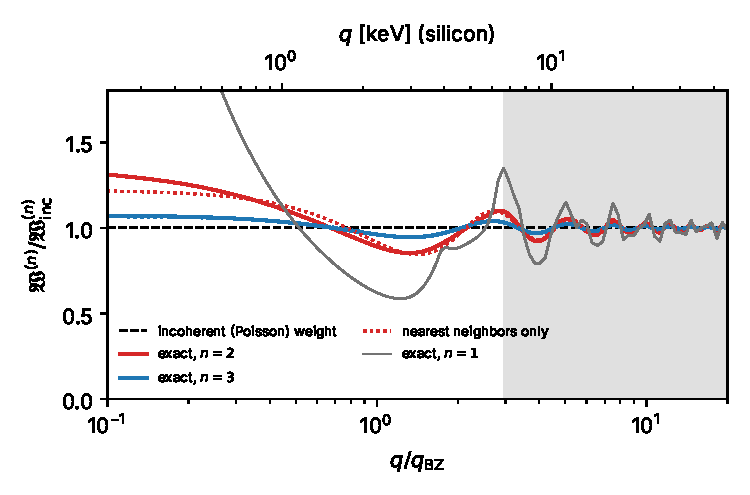
\includegraphics[width=\linewidth]{figures/ch11/limit11_3a.pdf}
\captionof{figure}{The exact $\omega$-integrated $n$-phonon weight of silicon at $T = 0$, \cref{eq:11.3-weight}, divided by its incoherent value, the Poisson weight of \cref{eq:11.3-inc} (dashed, one), averaged over the directions of $\vect{q}$, against $q/q_{\mathrm{BZ}}$, with $q_{\mathrm{BZ}} = \SI{2.25}{keV}$. For one species the couplings and the Debye--Waller factors cancel in the ratio, which is $1 + \delta^{\mathrm{coh}}_n(q)$ for any coupling of the form $\sum_\kappa c_\kappa n_\kappa$. Displacement correlations from the PBE force constants of \cref{sec:5.2} on a $48^3$ grid, pair sum to \SI{40}{\angstrom}, direction average exact. Solid: two (red) and three (blue) phonons. Dotted: the nearest-neighbor pairs alone, the leading correction. Thin gray: one phonon, which must be summed in reciprocal space. Gray band: $q \ge 2.95\,q_{\mathrm{BZ}} = \SI{6.6}{keV}$, where the two- and three-phonon weights stay within \SI{10}{\percent} of the incoherent ones. The three-phonon weight does so at every $q$, the one-phonon weight only above $7.9\,q_{\mathrm{BZ}}$.}\label{fig:11-limit-3a}
\par}
\smallskip
Below about three times the zone momentum the two-phonon weight differs from the Poisson weight by up to \SI{35}{\percent}, and pointwise in $\omega$ the incoherent spectrum misses the momentum conservation of the phonon pair even far above the zone.
\end{limitbox}

At small $q$ the phases are irrelevant, and every pair adds with the square of its correlation. The coherent two-phonon weight then exceeds the incoherent one by \SI{35}{\percent}, mostly from the four bonds, along which the longitudinal displacements of neighbors are correlated with a coefficient of 0.44 (a dynamical number, distinct from the geometric weight $j_{\mathrm{BZ}} \approx 0.44$ above, to which it is close by coincidence). Near $q_{\mathrm{BZ}}$ the bond phases turn the sign of this correction, and from about $3\,q_{\mathrm{BZ}}$ the correction oscillates with the period of the bond length and decays: $\delta^{\mathrm{coh}}_2 = -0.079$, $+0.014$, $-0.018$ and $-0.025$ at 2, 5, 10 and \SI{20}{keV}. The nearest-neighbor pairs alone account for 0.21 of the 0.35 at small $q$, and above about $2\,q_{\mathrm{BZ}}$ they follow the full curve within \SI{1}{\percent} of the weight. The three-phonon correction is smaller everywhere, since it carries the cube of a correlation coefficient below one: $-0.027$, $+0.016$, $-0.006$ and $-0.012$ at the same momentum transfers. The one-phonon term is the exception: it is sharp in $\omega$ at fixed $\vect{q}$, its pair sum does not converge absolutely, and its $\omega$-integrated weight approaches the incoherent value slowly, within \SI{10}{\percent} above about \SI{18}{keV}. Near each reciprocal-lattice vector the soft acoustic phonons enhance the one-phonon weight. Above $q_{\mathrm{BZ}}$, where \cref{eq:11.1-Sac} no longer holds, the one-phonon term is computed from \cref{eq:11.1-S1} with all branches and Umklapp terms, and its weight grows on average as $q^2\ee^{-2W_\kappa}$, the incoherent form, up to these corrections.

\Cref{fig:11-mph} shows the three parts of the silicon response at $q = \SI{10}{keV}$, the momentum transfer at which \cref{sec:8.5} placed the end of the one-phonon regime. One phonon carries a weight of 0.058 per nucleus, two phonons \num{1.8e-3} and three or more \num{4.0e-5}, close to the Poisson weights $2W_\kappa\ee^{-2W_\kappa} = 0.059$, $(2W_\kappa)^2\ee^{-2W_\kappa}/2 = \num{1.9e-3}$ and the rest. The exact one-phonon spectrum, averaged over directions, follows the projected density of states. The exact two-phonon spectrum follows the self-convolution of the single-phonon distribution within \SI{17}{\percent} in every bin of \SI{1}{meV} between 22 and \SI{120}{meV}, where the spectrum exceeds a tenth of its maximum; toward the edges of the band the ratio of the exact to the incoherent spectrum falls to about one half.

\begin{figure}[tbp]
  \centering
  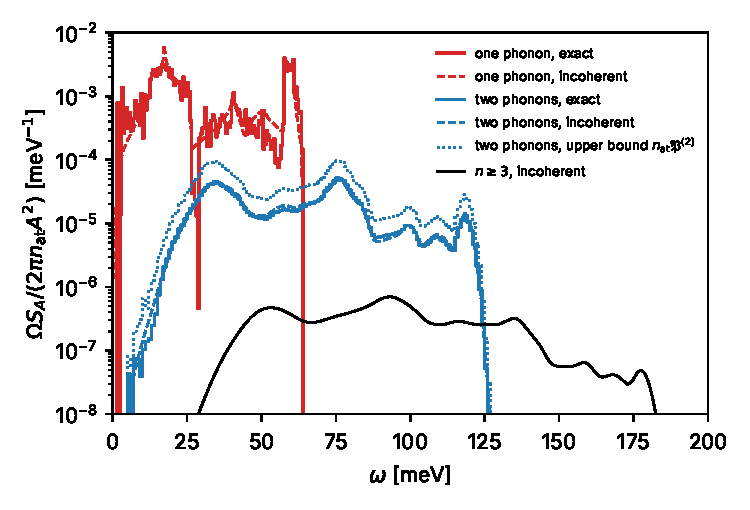
\includegraphics[width=\linewidth]{figures/ch11/fig11_3.pdf}
  \caption{Nuclear response of silicon at $|\vect{q}| = \SI{10}{keV}$ and $T = 0$, per nucleus, $\Omega S_A/(2\pi n_{\mathrm{at}}A^2)$, averaged over the directions of $\vect{q}$, split by the number of phonons; the elastic weight $\ee^{-2W_\kappa} = 0.939$ at $\omega = 0$ is not shown. Red: one phonon, exact (\cref{eq:11.1-S1}, all six branches, histogram of 0.5-meV bins) and incoherent (dashed). Blue: two phonons, exact (\cref{eq:11.3-Sn}, 1-meV bins), incoherent (dashed) and the upper end $n_{\mathrm{at}}\mathfrak{P}^{(2)}$ of the certified band \cref{eq:11.3-band} (dotted). Black: three or more phonons, incoherent. Phonons from the PBE force constants of \cref{sec:5.2}; incoherent parts from the density of states of the same force constants, with $\langle u_x^2\rangle = \SI{2.45e-3}{\angstrom^2}$. The exact two-phonon response is averaged over 240 wavevectors with $|\vect{q}|$ within \SI{1}{\percent} of \SI{10}{keV} on a $24^3$ grid commensurate with the zone, each rescaled to \SI{10}{keV} by $(10\,\mathrm{keV}/|\vect{q}|)^4$.}
  \label{fig:11-mph}
\end{figure}

\subsection{Exact phonon-order weights}

Integration over $\omega$ reduces the time integral of \cref{eq:11.3-exact} to the integrand at $t = 0$, and the $n$-phonon term becomes a sum over pairs of a static quantity. At $t = 0$ the two terms of \cref{eq:5.6-C} combine into $2n_{\vect{Q}\nu} + 1$, and the displacement correlation becomes the static correlation tensor
\begin{equation}
  B_{\kappa\kappa'}(\Delta\vect{R}) = \mathcal{C}_{\kappa\kappa'}(\Delta\vect{R},0) = \frac1N\sum_{\vect{Q}\nu}(2n_{\vect{Q}\nu} + 1)\,\frac{\vect{e}_{\kappa\nu}(\vect{Q})\,\vect{e}_{\kappa'\nu}(\vect{Q})^\dagger\,\ee^{\ii\vect{Q}\cdot\Delta\vect{R}}}{2\omega_{\vect{Q}\nu}\sqrt{M_\kappa M_{\kappa'}}} ,
  \label{eq:11.3-Bkk}
\end{equation}
whose on-site value $B_{\kappa\kappa}(\vect{0})$ is the displacement tensor $B_\kappa$ of \cref{eq:5.3-B}. Off site it measures how the displacements of two nuclei move together: $\langle u^\alpha_{\Delta\vect{R}\kappa}u^\beta_{\vect{0}\kappa'}\rangle$.
\begin{keyresult}[Exact $n$-phonon weight]
The $\omega$-integrated $n$-phonon response per cell is
\begin{equation}
  \mathfrak{W}^{(n)}(\vect{q}) = \Omega\int\frac{\dd\omega}{2\pi}\,S^{(n)}_A(\vect{q},\omega) = \frac{1}{n!}\sum_{\Delta\vect{R},\kappa,\kappa'}c_\kappa c_{\kappa'}\,\ee^{-\ii\vect{q}\cdot\Delta\vect{R}_{\kappa\kappa'}}\,\ee^{-W_\kappa - W_{\kappa'}}\,\bigl[\vect{q}\cdot B_{\kappa\kappa'}(\Delta\vect{R})\cdot\vect{q}\bigr]^n .
  \label{eq:11.3-weight}
\end{equation}
Its self terms are the incoherent weight $\mathfrak{W}^{(n)}_{\mathrm{inc}} = \sum_\kappa c_\kappa^2\,\ee^{-2W_\kappa}(2W_\kappa)^n/n!$, and $\delta^{\mathrm{coh}}_n(\vect{q}) = \mathfrak{W}^{(n)}/\mathfrak{W}^{(n)}_{\mathrm{inc}} - 1$ is the exact correction to the incoherent approximation for any energy window that contains the whole $n$-phonon band.
\end{keyresult}
\noindent A rate code applies this exact correction as a factor $1 + \delta^{\mathrm{coh}}_n$ per phonon order. At $T = 0$ the acoustic modes near $\mathrm{\Gamma}$ make $B_{\kappa\kappa'}(\Delta\vect{R})$ fall as $|\Delta\vect{R}|^{-2}$ at large distances (\cref{app:D.31}). Its square falls as $|\Delta\vect{R}|^{-4}$, faster than the number of pairs grows, and the sum converges absolutely for $n \ge 2$. For $n = 1$ the sum does not converge absolutely, and the one-phonon term is summed in reciprocal space, where it is \cref{eq:11.1-S1}. At $T > 0$ the thermal occupation of the same modes makes $B_{\kappa\kappa'}$ fall only as $T/|\Delta\vect{R}|$, and the two-phonon sum diverges; the subsection on thermal diffuse scattering resums it.

In silicon at $T = 0$ the correlation is short ranged in practice. With the force constants of \cref{sec:5.2} on a $48^3$ grid of wavevectors, the on-site value is $\langle u_x^2\rangle = \SI{2.45e-3}{\angstrom^2}$, as in \cref{we:5-dw}. The sum of \cref{eq:11.3-weight} to \SI{40}{\angstrom} takes seconds for any $\vect{q}$, and changes by less than $2\times10^{-3}$ beyond \SI{30}{\angstrom}. This sum produced the curves of \cref{fig:11-limit-3a}.

The $\omega$-integrated weight leaves open how the coherent correction is distributed in $\omega$. A pointwise statement follows from the structure of \cref{eq:11.3-Sn}, in which the coherent sum over the basis appears inside a squared modulus. By the Cauchy--Schwarz inequality, $|\sum_\kappa a_\kappa|^2 \le n_{\mathrm{at}}\sum_\kappa|a_\kappa|^2$ for the $n_{\mathrm{at}}$ nuclei of a cell, term by term in the sum over phonons. The \emph{momentum-resolved self density} $\mathfrak{P}^{(n)}(\vect{q},\omega)$ is \cref{eq:11.3-Sn} with the squared modulus replaced by the sum of the squared amplitudes of the single nuclei: the response of independent nuclei whose $n$ phonons must still add up to the crystal momentum $\vect{q}$. For silicon, $n_{\mathrm{at}} = 2$, and with $a_1$, $a_2$ the amplitudes of the two nuclei of a cell for one set of phonons, $|a_1 + a_2|^2 = 2(|a_1|^2 + |a_2|^2) - |a_1 - a_2|^2 \le 2(|a_1|^2 + |a_2|^2)$, with equality when the two nuclei move in phase.
\begin{keyresult}[Certified band]
At every $\vect{q}$, $\omega$ and $n$,
\begin{equation}
  \begin{gathered}
  0 \le S^{(n)}_A(\vect{q},\omega) \le n_{\mathrm{at}}\,\mathfrak{P}^{(n)}(\vect{q},\omega) , \\
  \frac{\Omega}{(2\pi)^3}\int_{\mathrm{BZ}}\dd^3p\;\mathfrak{P}^{(n)}(\vect{q} + \vect{p},\omega)\Big|_{\text{vertex at }\vect{q}} = S^{\mathrm{inc},(n)}_A(\vect{q},\omega) ,
  \end{gathered}
  \label{eq:11.3-band}
\end{equation}
where the average holds the factors $\vect{q}\cdot\vect{e}$ and $\ee^{-W_\kappa}$ at $\vect{q}$ and moves only the momentum constraint (\cref{app:D.31}), and $S^{\mathrm{inc},(n)}_A$ is the term of order $n$ of \cref{eq:11.3-inc}.
\end{keyresult}
\noindent For a lattice with one atom per cell the two sides of the inequality coincide, $S^{(n)}_A = \mathfrak{P}^{(n)}$, and the only error of the incoherent approximation is the momentum constraint, which the zone average removes. The constraint matters at the edges of each phonon band: the lowest two-phonon energies need two soft acoustic phonons, both near $\mathrm{\Gamma}$, and hence $\vect{q}$ near a reciprocal-lattice vector. At other $\vect{q}$ the exact spectrum vanishes at those energies, where the self density does not, and the lower end of the certified band is reached. For a crystal with a basis the certified band is wider by the factor $n_{\mathrm{at}}$. In silicon at \SI{10}{keV} its upper end reaches 2.7 times the incoherent two-phonon spectrum (\cref{fig:11-mph}): the certified band bounds the error, but it is too wide to test the incoherent spectrum point by point below a few $q_{\mathrm{BZ}}$; that test needs \cref{eq:11.3-Sn} itself.

\subsection{Thermal diffuse scattering}

In a warm crystal the scattered intensity of X-rays and neutrons does not drop to zero between the Bragg peaks. Thermal phonons fill the space around each peak with a diffuse cloud, which crystallographers subtract when they measure structure factors. The first-order part of the diffuse cloud is the one-phonon response at $\vect{q} = \vect{G} + \vect{k}$ with a soft acoustic phonon of wavevector $\vect{k}$. By \cref{eq:11.1-S1} its weight carries $(2n_{\vect{k}\nu} + 1)/\omega_{\vect{k}\nu} \approx 2T/(c_\nu k)^2$, and it grows as $1/|\vect{q} - \vect{G}|^2$ toward the peak. The second-order part comes from two soft phonons whose wavevectors add up to $\vect{k}$. It is milder, and it is exactly the term whose real-space sum diverged above.

In reciprocal space the two-phonon weight is finite. It is an average over one wavevector $\vect{Q}_1$ of the zone, with $\vect{Q}_2 = \vect{k} - \vect{Q}_1$; each thermal factor $(2n + 1)/2\omega \approx T/\omega^2$ is integrable around $\vect{Q} = 0$, and the average is singular only when both phonons are soft at once, as $\vect{k} \to 0$ (\cref{app:D.31}). The thermal part of the weight therefore obeys
\begin{equation}
  \mathfrak{W}^{(2),\mathrm{th}}(\vect{q}) \le \Bigl|\sum_\kappa c_\kappa\,\ee^{-W_\kappa}\,\ee^{\ii\vect{G}\cdot\vect{\tau}_\kappa}\Bigr|^2\,\frac{\Omega\,T^2q^4}{16\,M_{\mathrm{cell}}^2\,c_{\mathrm{min}}^4\,|\vect{q} - \vect{G}|} + (\text{terms regular at } \vect{q} = \vect{G}) ,
  \label{eq:11.3-tds}
\end{equation}
with $c_{\mathrm{min}}$ the lowest acoustic speed, \SI{4.67}{km.s^{-1}} in silicon for the transverse wave along $[110]$ polarized along $[1\bar10]$. The singularity is integrable, and it is weighted by the Bragg structure factor: it vanishes near a reflection that the basis extinguishes, such as (200) in silicon. In the classical limit the singular part is exactly proportional to $1/|\vect{q} - \vect{G}|$. Its coefficient lies below the bound and depends on the direction of $\vect{q} - \vect{G}$ relative to $\vect{q}$; for an isotropic medium with the speeds of silicon and $\vect{q} - \vect{G}$ parallel to $\vect{q}$ it is 0.46 of the bound. This $1/|\vect{q} - \vect{G}|$ law, against the $1/|\vect{q} - \vect{G}|^2$ of the first order, is the classical result for second-order thermal diffuse scattering~\cite{warren1969xray}. On the truncation label this second-order term is $\mathcal{K}$ = multiphonon (two phonons, coherent) at $n_T = 2$, since the singular part is quadratic in the occupation numbers; the cross terms linear in $n_{\vect{Q}\nu}$, at $n_T = 1$, are at most logarithmically singular.

\begin{limitbox}[Second-order thermal diffuse scattering][lim:11.3b]
Near a reciprocal-lattice vector $\vect{G}$ of a warm crystal, two soft acoustic phonons give the $\omega$-integrated response a singular part that falls as $1/|\vect{q} - \vect{G}|$, weighted by the structure factor at $\vect{G}$ and by $T^2$~\cite{warren1969xray}; its bound is \cref{eq:11.3-tds}.
\par\smallskip
{\centering
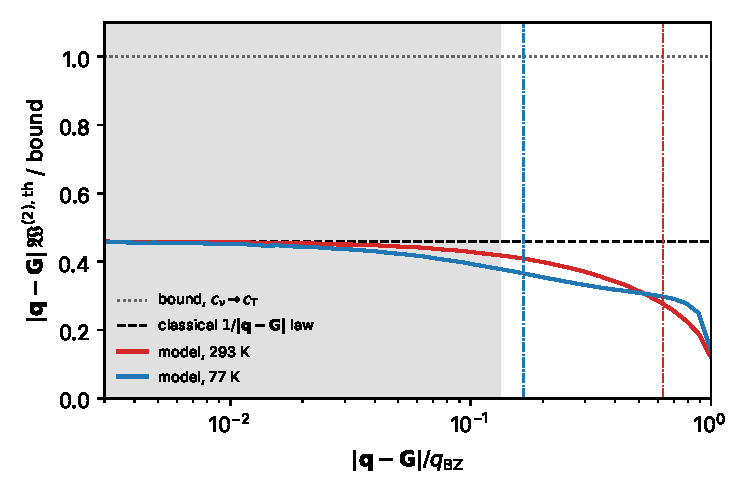
\includegraphics[width=\linewidth]{figures/ch11/limit11_3b.pdf}
\captionof{figure}{Thermal two-phonon weight times $|\vect{q} - \vect{G}|$, in units of the bound \cref{eq:11.3-tds} with $c_{\mathrm{min}}$ replaced by the transverse speed (dotted, one), for $\vect{G} = \vect{G}_{111}$ of silicon and $\vect{q} - \vect{G}$ parallel to $\vect{q}$, against $|\vect{q} - \vect{G}|/q_{\mathrm{BZ}}$. Model: isotropic elastic medium with the speeds $v_L = [(B + \frac43G)/\rho_T]^{1/2} = 8.95$ and $v_T = (G/\rho_T)^{1/2} = \SI{5.34}{km.s^{-1}}$ of silicon, with $G$ the Hill shear modulus, the mean of the Voigt value $G_{\mathrm{V}} = (C_{11} - C_{12} + 3C_{44})/5 = \SI{68.0}{GPa}$ and the Reuss value $G_{\mathrm{R}} = 5(C_{11} - C_{12})C_{44}/[4C_{44} + 3(C_{11} - C_{12})] = \SI{64.9}{GPa}$, exactly longitudinal and transverse polarizations, wavevectors cut at $|\vect{Q}| < q_{\mathrm{BZ}}$, and the full thermal factors $\coth(\omega_1/2T)\coth(\omega_2/2T) - 1$. Dashed: the classical $1/|\vect{q} - \vect{G}|$ law, 0.46 of the bound. Solid: the model at \SI{293}{K} (red) and \SI{77}{K} (blue). Dash-dotted: the boundary $|\vect{q} - \vect{G}| = T/c_{\mathrm{T}}$ of the classical soft pair at each temperature. Gray: within \SI{10}{\percent} of the classical law at \SI{293}{K}, $|\vect{q} - \vect{G}| \le 0.13\,q_{\mathrm{BZ}}$; at \SI{77}{K} the same holds below $0.065\,q_{\mathrm{BZ}}$. At \SI{10}{mK} the boundary lies at $2\times10^{-5}\,q_{\mathrm{BZ}}$.}\label{fig:11-limit-3b}
\par}
\smallskip
The law needs both phonons to be classical, $c_\nu|\vect{q} - \vect{G}| \ll T$. Farther from the peak the thermal occupations fall off and the weight drops below the law, and at the zone scale the dispersion and the regular two-phonon terms dominate.
\end{limitbox}

In a dark-matter detector the second-order thermal diffuse scattering is negligible. At \SI{10}{mK} the classical region ends at $|\vect{q} - \vect{G}| = T/c_{\mathrm{T}} = \SI{48}{meV}$, with the transverse speed $c_{\mathrm{T}}$ of \cref{lim:11.3b}, and the coefficient, which carries $T^2$, is $10^{-9}$ of its room-temperature value. The second-order term matters for the X-ray and neutron data, taken warm, that calibrate the lattice response, and for any rate quoted at \SI{77}{K} or above. At room temperature, a tenth of the zone momentum away from the (111) peak of silicon, the singular thermal weight is as large as the whole incoherent two-phonon weight there, 1.07 times it in the model of the limit check. A calculation at $T > 0$ evaluates the two-phonon coherence in reciprocal space and never as the real-space sum of \cref{eq:11.3-weight}.

\subsection{The charge vertex at large momentum}

For a coupling to charge, the dark photon of \cref{sec:11.2}, the electrons are part of the vertex, and $c_\kappa$ is no longer a number. Every result of this section assumed that $c_\kappa$ is a number; for a coupling to nucleons this assumption is exact, since the nucleons move with their nucleus. At momentum transfers small compared with the zone the electrons follow the nuclei adiabatically, and their effect is the Born effective charge and the screening of \cref{sec:11.2}. Far above the zone the question is how much of the electron cloud a displaced atom carries along, at the momentum transfer $q$ itself. A rigid neutral atom contributes $Z_\kappa - f_\kappa(q)$, with $f_\kappa$ the form factor of its electron cloud (\cref{sec:8.6}), and what the rigid atom misses is the deformation of the electron density as the atom moves. The deformation obeys one exact constraint. Summed over the atoms of a cell, for a displacement that is the same in every cell, the deformation is the change of the electron density under a uniform translation of the crystal. At the Fourier component $\vect{G}$ this change is $\ii G_\alpha$ times the density component itself, since with $n_e(\vect{q}) = \sum_j\ee^{\ii\vect{q}\cdot\vect{r}_j}$ a translation by $\vect{u}$ multiplies that component by $\ee^{\ii\vect{G}\cdot\vect{u}}$. The core shells follow their nucleus closely, polarized by the small residual field at the nucleus. The valence share is the open problem. It is not known how fast the deformation of the bonding charge decays between about 3 and \SI{20}{keV}: a calculation with pseudopotentials gives densities that are unphysical inside the core radius, above about \SI{10}{keV} in silicon, and a free-atom model has no bonds. The answer needs an all-electron calculation of displaced atoms in a large cell, with the translation sum rule as its test. Until that calculation is done, the multiphonon response of a charge coupling far above the zone rests on the rigid-atom vertex as an assumption, while that of a nucleon coupling does not.

\section{Impulse limit and free nuclear recoil}\label{sec:11.4}

A dark-matter particle of \SI{20}{MeV} can transfer up to $2\mchi v_{\mathrm{max}} = \SI{106}{keV}$ to a silicon nucleus. At $q = \SI{100}{keV}$ the free recoil energy is $E_R = \SI{191}{meV}$, three times the highest phonon energy, and the Poisson series of \cref{sec:11.3} has a mean of $2W_\kappa = 6.3$ phonons. Their sum is no longer a set of phonon bands. It is a single peak centered at $E_R$, \SI{88}{meV} wide, and as $q$ grows it narrows toward the delta function $\delta(\omega - E_R)$ of the free recoil that \cref{sec:1.3,sec:2.2} assumed. The nucleus recoils almost as if it were free, and what is left of the crystal is the motion of the nucleus in its well at the moment of the kick, which Doppler-broadens the line by an amount set by the kinetic energy of the nuclei; the standard nuclear-recoil rate with the Helm form factor is its limit, reached in silicon above 90 to \SI{140}{keV} depending on the criterion.

\subsection{The impulse approximation}

At $q = \SI{100}{keV}$, 44 times the zone momentum, the distinct part of the response is negligible (\cref{sec:11.3}), and each nucleus responds on its own. Its self correlation has an exact form that needs no phonons. The kick $\ee^{\ii\vect{q}\cdot\vect{X}}$ shifts the momentum of the nucleus by $\vect{q}$, and since every interaction in the crystal depends on the positions of the nuclei and not on their momenta, the kick changes only the kinetic energy $\vect{p}^2/2M_\kappa$. The Hamiltonian seen after the kick is the old one plus
\begin{equation*}
  D = E_R + \frac{\vect{q}\cdot\vect{p}}{M_\kappa} ,
\end{equation*}
the energy that the same kick would give a free particle of momentum $\vect{p}$. Its mean and variance follow exactly (\cref{app:D.32}). The mean energy deposited is $\langle D\rangle = E_R$, the sum rule \cref{eq:5.6-sum}. The variance is $\langle D^2\rangle - E_R^2 = q^2\langle p_{\hat q}^2\rangle/M_\kappa^2$, with $p_{\hat q} = \hat{\vect{q}}\cdot\vect{p}$, at any temperature and for any potential, anharmonic ones included. Defining the kinetic energy of the nucleus along the direction of the kick, $E^{\mathrm{kin}}_\kappa(\hat{\vect{q}}) = \langle p_{\hat q}^2\rangle/2M_\kappa$, the width of the response is
\begin{equation}
  \sigma_\omega = \bigl[4E_R\,E^{\mathrm{kin}}_\kappa(\hat{\vect{q}})\bigr]^{1/2} .
  \label{eq:11.4-width}
\end{equation}

If the nucleus were free, $D$ would commute with the Hamiltonian, and each momentum $\vect{p}$ would absorb exactly the energy $D$. For a bound nucleus the commutator is the force of the neighbors, and the \emph{impulse approximation} drops it: the nucleus is treated as free for the duration of the kick, with the momentum distribution $\mathfrak{f}_\kappa(\vect{p})$ that it has in the crystal, normalized to one.
\begin{keyresult}[Impulse approximation of the nuclear response]
\begin{equation}
  S_A(\vect{q},\omega) \simeq \frac{2\pi}{\Omega}\sum_\kappa c_\kappa^2\int\dd^3p\;\mathfrak{f}_\kappa(\vect{p})\;\delta\Bigl(\omega - \frac{q^2}{2M_\kappa} - \frac{\vect{q}\cdot\vect{p}}{M_\kappa}\Bigr) .
  \label{eq:11.4-IA}
\end{equation}
It keeps the exact mean $E_R$ and the exact width \cref{eq:11.4-width}. Its leading error is the third cumulant, at $T = 0$ equal to $c_3 = (q^2/2M_\kappa^2)\langle\partial_{\hat q}^2V\rangle$ with $V$ the Born--Oppenheimer surface, whose share of the shape falls as $1/q$ (\cref{app:D.32}).
\end{keyresult}
\noindent The term $\vect{q}\cdot\vect{p}/M_\kappa$ is a Doppler shift: a nucleus moving toward the kick absorbs more energy, one moving away absorbs less. The same picture underlies the impulse approximation of the electrons in \cref{we:4-gas}, where the Fermi momentum takes the place of the zero-point momentum, and neutron Compton scattering, which uses it to measure the momentum distributions of light nuclei in solids and liquids~\cite{andreani2005measurement}. The approximation is good when the kick is short compared with a vibration period. The time integral of the response is cut off at $t \sim 1/\sigma_\omega$, and the force of the neighbors changes the momentum during that time by a fraction $\sim\langle\omega\rangle/\sigma_\omega$ of its spread. At $T = 0$ this fraction is $x_R^{-1/2}$, with the recoil parameter $x_R = E_R/\langle\omega\rangle$ of \cref{sec:8.5}.

In a harmonic crystal $\mathfrak{f}_\kappa$ is a Gaussian at any temperature, since the momentum of each mode is Gaussian in a thermal state of an oscillator. Its width follows from the displacement correlation \cref{eq:5.6-C}. On a site of cubic symmetry, with the projected density of states $g_{\mathrm{ph},\kappa}/3$ of \cref{sec:11.3},
\begin{equation*}
  E^{\mathrm{kin}}_\kappa = \frac14\int\dd\omega\;\frac{g_{\mathrm{ph},\kappa}(\omega)}{3}\;\omega\coth\frac{\omega}{2T} ,
\end{equation*}
which at $T = 0$ is $\langle\omega\rangle/4$. Half the zero-point energy of each mode is kinetic, so a nucleus carries the kinetic energy $3\langle\omega\rangle/4$, a third of it along each direction. The impulse response of one species is then the Gaussian
\begin{equation}
  S_A(\vect{q},\omega) \simeq \frac{2\pi c_\kappa^2}{\Omega}\,\frac{1}{(2\pi\sigma_\omega^2)^{1/2}}\exp\Bigl[-\frac{(\omega - E_R)^2}{2\sigma_\omega^2}\Bigr] , \qquad
  \sigma_\omega^2 = E_R\,\Bigl\langle\omega\coth\frac{\omega}{2T}\Bigr\rangle ,
  \label{eq:11.4-IAgauss}
\end{equation}
which at $T = 0$ has $\sigma_\omega/E_R = x_R^{-1/2}$, the relative width that \cref{sec:8.5} found from the cumulants of the Poisson series. Campbell-Deem, Knapen, Lin and Villarama obtain it as the saddle point of the time integral at $t = 0$~\cite[Eqs.~(37)--(39)]{campbelldeem2022dark}. For a nucleus in an isotropic oscillator of frequency $\omega_0$, the spread $q(\omega_0/2M_\kappa)^{1/2}$ of Kahn, Krnjaic and Mandava~\cite[Eq.~(4)]{kahn2021dark} is the same width with $\langle\omega\rangle = \omega_0$. The harmonic crystal gives every cumulant (\cref{app:D.32}): $c_k = E_R\langle\omega^{k-1}\rangle$ for odd $k$, at any temperature, and $c_k = E_R\langle\omega^{k-1}\coth(\omega/2T)\rangle$ for even $k$. The skewness, $c_3/\sigma_\omega^3 = (\langle\omega^2\rangle/\langle\omega\rangle^2)\,x_R^{-1/2}$ at $T = 0$, is the leading correction to \cref{eq:11.4-IAgauss}. It moves the maximum of the spectrum below $E_R$ by about half the skewness times $\sigma_\omega$, while the mean stays at $E_R$.

In silicon the density of states of \cref{sec:5.2} gives $\langle\omega\rangle = \SI{40.9}{meV}$, so $E^{\mathrm{kin}}_\kappa = \SI{10.2}{meV}$ at $T = 0$, and $\langle\omega^2\rangle/\langle\omega\rangle^2 = 1.19$. The zero-point motion broadens the line as much as a classical gas at \SI{237}{K} would, the temperature at which $T/2$ equals $E^{\mathrm{kin}}_\kappa$. Heating the crystal changes this little until the thermal energy reaches the phonon energies: $E^{\mathrm{kin}}_\kappa$ rises by \SI{2}{\percent} at \SI{77}{K} and by \SI{56}{\percent} at \SI{300}{K}, where the width is 1.25 times its zero-temperature value. At the \SI{10}{mK} of a detector the zero-temperature values hold.

\Cref{fig:11-impulse} follows the silicon response from the multiphonon regime into the impulse regime. At $q = \SI{50}{keV}$, $x_R = 1.2$, the spectrum still shows the phonon bands: its maximum lies at $0.36\,E_R = \SI{17}{meV}$, on the transverse-acoustic peak of the single-phonon distribution, and a fifth of the weight is in the zero-phonon line. At \SI{100}{keV} the bands have merged into a peak whose maximum lies at $0.81\,E_R$. The Gaussian \cref{eq:11.4-IAgauss} has the right height and width there, and it misses by up to a fifth of the peak height, from the skewness and from the remaining structure of the phonon orders. At 200 and \SI{400}{keV} the deviations fall to 7 and \SI{3}{\percent} of the peak, roughly as $x_R^{-1/2}$, and the maximum approaches $E_R$.

\begin{figure}[tbp]
  \centering
  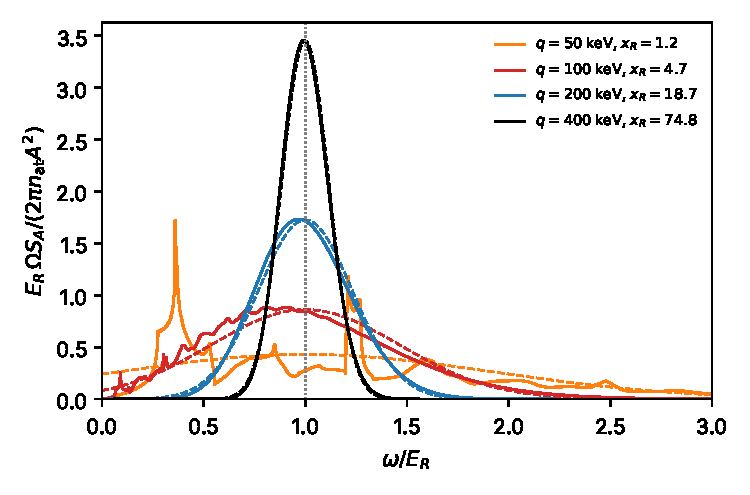
\includegraphics[width=\linewidth]{figures/ch11/fig11_4.pdf}
  \caption{Nuclear response of silicon at $T = 0$ per nucleus, $\Omega S_A/(2\pi n_{\mathrm{at}}A^2)$, times $E_R$, against $\omega/E_R$, at $q = 50$, 100, 200 and \SI{400}{keV} ($x_R = 1.2$, 4.7, 18.7 and 74.8). Solid: the incoherent response of \cref{eq:11.3-inc} summed over all phonon orders, from the density of states of the PBE force constants of \cref{sec:5.2}. It is evaluated by Fourier transform of the generating formula \cref{eq:5.6-gen}. The zero-phonon line, of weight $\ee^{-2W_\kappa} = 0.21$ at \SI{50}{keV} and below $2\times10^{-3}$ at the larger $q$, is not shown. Dashed: the impulse Gaussian \cref{eq:11.4-IAgauss}, mean $E_R$ and relative width $x_R^{-1/2}$. Dotted: the free recoil, $\omega = E_R$. The maximum of the spectrum lies at 0.36, 0.81, 0.97 and $0.99\,E_R$.}
  \label{fig:11-impulse}
\end{figure}

The width needs one number per species, the kinetic energy of the nucleus along $\hat{\vect{q}}$. The harmonic value comes from the same phonon calculation as the Debye--Waller exponent (\cref{sec:5.4,app:E.4}), as the first moment of the projected density of states instead of the inverse moment. Beyond the harmonic approximation the nuclear momentum distribution, its kinetic energy and the curvature that sets $c_3$ are computed by path-integral molecular dynamics, which treats the nuclei as quantum particles on the full Born--Oppenheimer surface; \cref{app:E.17} specifies that calculation for silicon, germanium and GaAs. The anharmonic change of $E^{\mathrm{kin}}_\kappa$ is the subject of \cref{sec:11.5}.

\begin{workedexample}{The impulse width at \SI{100}{keV} in silicon}\label{we:11-width}
Take a silicon nucleus, $M = \SI{26.162}{GeV}$, at $T = 0$ and $q = \SI{100}{keV}$. The free recoil energy is $E_R = q^2/2M = \SI{191.1}{meV}$, and with $\langle\omega\rangle = \SI{40.9}{meV}$ the recoil parameter is $x_R = 4.67$. The kinetic energy along $\hat{\vect{q}}$ is $\langle\omega\rangle/4 = \SI{10.23}{meV}$, and \cref{eq:11.4-width} gives
\begin{equation*}
  \sigma_\omega = (4 \times \SI{191.1}{meV} \times \SI{10.23}{meV})^{1/2} = \SI{88.4}{meV} , \qquad \frac{\sigma_\omega}{E_R} = 0.463 = x_R^{-1/2} .
\end{equation*}
The Doppler reading gives the same number. The nucleus moves along $\hat{\vect{q}}$ with the root-mean-square speed $(2E^{\mathrm{kin}}_\kappa/M)^{1/2} = \SI{265}{m.s^{-1}}$, while the kick gives it $q/M = \SI{1.15}{km.s^{-1}}$. The relative spread of $D$ is twice the ratio of the two speeds, 0.463.

The Gaussian has a full width at half maximum of \SI{208}{meV}, larger than $E_R$ itself. The full response of \cref{fig:11-impulse} at this $q$ has a width at half maximum of \SI{207}{meV}. The shape is skewed. The skewness is $1.19 \times 4.67^{-1/2} = 0.55$, which places the maximum about $0.55\,\sigma_\omega/2 = \SI{24}{meV}$ below $E_R$; the full response peaks at \SI{154}{meV}, \SI{37}{meV} below, because the phonon orders still leave ripples on the peak. At \SI{300}{K} the width grows to \SI{110}{meV}.

A germanium nucleus is 2.6 times heavier and its phonons are softer. With $\langle\omega\rangle \approx \SI{23.6}{meV}$, an estimate from its Debye temperature of \SI{373}{K} (below), the same $q$ gives $E_R = \SI{73.9}{meV}$, $x_R = 3.1$ and $\sigma_\omega/E_R = 0.57$: at equal momentum transfer the germanium response is further from free recoil than the silicon one.
\end{workedexample}

On the truncation label of \cref{sec:8.5}, \cref{eq:11.4-IA} is $\mathcal{K}$ = impulse with $n_B = 0$. It holds at any anharmonic order $n_A$ when $\mathfrak{f}_\kappa$ is the true momentum distribution, and the Gaussian \cref{eq:11.4-IAgauss} is its value at $n_A = 0$. Temperature enters only through $E^{\mathrm{kin}}_\kappa$, with all orders $n_T$ kept by the factor $\coth(\omega/2T)$.

\subsection{Free recoil and the standard rate}

As $x_R$ grows, the relative width $x_R^{-1/2}$ goes to zero and the Gaussian becomes $\delta(\omega - E_R)$~\cite[Eq.~(42)]{campbelldeem2022dark}. For a coupling to nucleons the vertex of a nucleus is $A_\kappa F_N(q)$, with the elastic form factor $F_N$ of \cref{eq:2.2-FN}. The nucleons move with their nucleus, and the momenta of the impulse regime, up to a few MeV for sub-GeV dark matter, are far too small to excite it internally. For one species the response is then $S_A = 2\pi\nd_NA^2F_N(q)^2\delta(\omega - q^2/2M)$, with $\nd_N = n_{\mathrm{at}}/\Omega$ the number density of nuclei. Insert it into \cref{eq:8.2-spectrum} with one row, $\mathfrak{D} = |\tilde V_N|^2$. The response does not depend on $\hat{\vect{q}}$, so the angle between $\vect{q}$ and $\vect{v}$ can be integrated first: $\int\dd^3q/(2\pi)^3$ of $\delta(\omega - \vect{q}\cdot\vect{v} + q^2/2\mchi)$ gives $\int q\,\dd q\,\Theta(v - \vmin)/(4\pi^2v)$, as in \cref{sec:1.3}, and the average over $f_\chi$ turns $\Theta/v$ into $\eta(\vmin)$ of \cref{eq:1.3-eta}. With $\rho_T = \nd_NM$,
\begin{equation*}
  \frac{\dd\mathcal{R}}{\dd\omega} = \frac{\rho_\chi}{\mchi\,\nd_NM}\int\frac{q\,\dd q}{4\pi^2}\,|\tilde V_N|^2\,2\pi\nd_NA^2F_N^2\,\delta\Bigl(\omega - \frac{q^2}{2M}\Bigr)\,\eta(\vmin)
  = \frac{\rho_\chi A^2|\tilde V_N|^2}{2\pi\mchi}\,F_N(q)^2\,\eta(\vmin) ,
\end{equation*}
at $q = (2M\omega)^{1/2}$, and \cref{eq:1.3-vmin} with $\Delta_\chi = 0$ gives $\vmin = q/2M + q/2\mchi = q/2\mu_{\chi N}$. A heavy mediator, $|\tilde V_N|^2 = \pi\sigma_p/\mu_{\chi p}^2$, with $\sigma_N = \sigma_pA^2\mu_{\chi N}^2/\mu_{\chi p}^2$ from \cref{eq:2.2-nucleus}, gives
\begin{keyresult}[Free nuclear recoil as the impulse limit]
\begin{equation}
  \frac{\dd\mathcal{R}}{\dd E_R} = \frac{\rho_\chi\,\sigma_N}{2\mchi\,\mu_{\chi N}^2}\,F_N(q)^2\,\eta(\vmin) , \qquad q = (2ME_R)^{1/2} , \qquad \vmin = \frac{q}{2\mu_{\chi N}} ,
  \label{eq:11.4-LS}
\end{equation}
the spin-independent recoil spectrum of \cref{sec:2.2}, with $\sigma_N$ of \cref{eq:2.2-nucleus}. It is the limit $x_R \to \infty$ of the crystal response.
\end{keyresult}
\noindent This is the standard rate of nuclear-recoil searches~\cites{lewin1996review}[Eq.~(104)]{lin2019tasi}, and with $F_N$ the Helm form \cref{eq:2.2-helm} and the Lewin--Smith parameters of \cref{sec:2.2} it is the rate that experiments quote. Kahn and Lin reach the same spectrum from an Einstein oscillator, whose Poisson distribution of phonon numbers concentrates at $E_R/\omega_0$ for large $q$~\cite[Sect.~IV\,A, Eqs.~(90)--(92)]{kahn2022searches}. On the truncation label the free recoil is $\mathcal{K}$ = impulse at zero width, $n_B = 0$; its mean deposit is exact at every anharmonic order and temperature, and only the width depends on them.

The derivation says what the formula needs: a recoil parameter large enough that the response is a narrow peak, and a rate whose weight in $\omega$, the factor $\eta(\vmin)$ together with the threshold, does not vary across the width $\sigma_\omega$. \Cref{lim:11.4a} tests both in silicon, by computing the heavy-mediator rate from the full multiphonon response and dividing it by \cref{eq:11.4-LS}. For a particle of \SI{1}{GeV}, whose kinematic endpoint lies far above the energies shown, the two agree within \SI{10}{\percent} for $x_R \ge 2.3$, or $E_R \ge \SI{93}{meV}$ and $q \ge \SI{70}{keV}$, and within \SI{2}{\percent} for $x_R \ge 4.3$. The free form works where the spectrum is not yet narrow, as Campbell-Deem and collaborators observed~\cite[Sect.~III\,D]{campbelldeem2022dark}, because a smooth weight averages over the peak and the mean of the peak is exactly $E_R$. Below $x_R \approx 2$ the deposit comes in whole phonons, and the ratio swings by factors of two with the bands of the phonon spectrum.

A lighter particle has its endpoint $2\mu_{\chi N}^2v_{\mathrm{max}}^2/M$ close to the energies that matter, and there $\eta$ falls steeply across the peak. For \SI{50}{MeV} the endpoint is at \SI{1.34}{eV}, $x_R = 32.7$. Between $x_R = 3$ and 8 the free form overestimates the crystal rate by 5 to \SI{21}{\percent}, because the width spreads each momentum transfer over a range of energies across which $\eta$ falls steeply. From $x_R = 14$ upward, however, $4.9\,\sigma_\omega$ below the endpoint, the crystal rate exceeds the free one by more than \SI{10}{\percent} and keeps rising. Above the endpoint the free recoil gives nothing, while the Doppler tail of the bound nucleus still deposits energy. This is the impulse-regime counterpart of the Poisson tail of \cref{we:11-tail}, and the reason Kahn, Krnjaic and Mandava found that a bound nucleus extends the reach of a detector below the masses that elastic kinematics allows~\cite[text after Eq.~(4)]{kahn2021dark}. The impulse Gaussian \cref{eq:11.4-IAgauss}, used in the same rate integral, follows the full crystal result within \SI{5}{\percent} from $x_R \approx 3.6$ at \SI{1}{GeV} and 3.8 at \SI{50}{MeV}, up to three quarters of the endpoint, and it captures the endpoint tail too.

\begin{limitbox}[Free nuclear recoil with the Helm form factor][lim:11.4a]
For $x_R \gg 1$ the nuclear response becomes $(2\pi/\Omega)\sum_\kappa c_\kappa^2\delta(\omega - q^2/2M_\kappa)$~\cite[Eqs.~(39), (42)]{campbelldeem2022dark}, and the rate is the free recoil \cref{eq:11.4-LS} with $F_N = F_{\mathrm{Helm}}$ and the Lewin--Smith parameters~\cites{lewin1996review}[Eq.~(104)]{lin2019tasi}.
\par\smallskip
{\centering
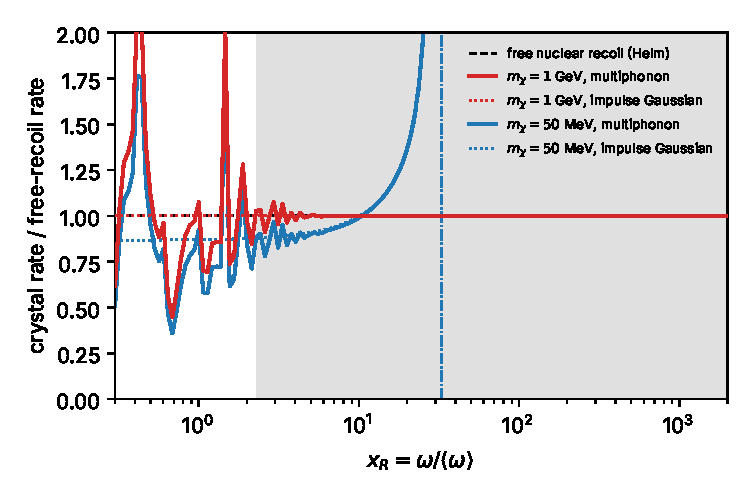
\includegraphics[width=\linewidth]{figures/ch11/limit11_4a.pdf}
\captionof{figure}{Heavy-mediator recoil rate of silicon per unit mass from the crystal response, divided by the free-recoil rate \cref{eq:11.4-LS} at $E_R = \omega$, against $x_R = \omega/\langle\omega\rangle$ with $\langle\omega\rangle = \SI{40.9}{meV}$. Solid: incoherent multiphonon response at $T = 0$, all orders, from the PBE density of states of \cref{sec:5.2}, integrated over $q$ with $\eta(\vmin)$ of the halo of \cref{sec:1.2} and the Helm form factor, for $\mchi = \SI{1}{GeV}$ (red) and \SI{50}{MeV} (blue). Dotted: the same with the impulse Gaussian \cref{eq:11.4-IAgauss}, the leading correction. Dash-dotted: the free-recoil endpoint at \SI{50}{MeV}. Gray band: $x_R \ge 2.3$, where the \SI{1}{GeV} rate stays within \SI{10}{\percent} of the free one. The lighter particle departs from it within about five widths $\sigma_\omega$ of its endpoint.}\label{fig:11-limit-4a}
\par}
\smallskip
Below $x_R \approx 2$ the energy arrives in whole phonons and the rate follows the phonon bands; near the kinematic endpoint the Doppler width of the bound nucleus feeds energies that a free nucleus cannot reach.
\end{limitbox}

Where does the impulse regime begin? The onset depends on the criterion. The relative width $x_R^{-1/2}$ falls to one half at $x_R = 4$, where the impulse Gaussian reproduces the rate of the limit check within \SI{5}{\percent}. This is $q = 2(2M\langle\omega\rangle)^{1/2}$, the boundary above which Campbell-Deem and collaborators replace the multiphonon sum by the Gaussian~\cite[text after Eq.~(39)]{campbelldeem2022dark}. In silicon it lies at $q = \SI{92.5}{keV}$, $E_R = \SI{164}{meV}$. The stricter criterion of \cref{sec:8.5}, a width below a third of $E_R$, needs $x_R \ge 9$, at \SI{139}{keV} and \SI{0.37}{eV}. For germanium a rough $\langle\omega\rangle$ is enough, and its Debye temperature of \SI{373}{K} supplies one (\cref{tab:5-phonons}): the Debye mean $\frac34\omega_{\mathrm{D}} = \SI{24.1}{meV}$, scaled by the ratio 0.981 of the computed to the Debye mean in silicon, gives $\langle\omega\rangle \approx \SI{23.6}{meV}$. The onsets are then $q = \SI{113}{keV}$ and $E_R = \SI{95}{meV}$ at $x_R = 4$, and \SI{170}{keV} and \SI{0.21}{eV} at $x_R = 9$. The heavier nucleus needs a larger momentum transfer but a smaller recoil energy. These onsets are not the \SI{93.4}{keV} of \cref{we:11-tail}, which is the momentum at which a free nucleus would first deposit three Debye energies. A particle much lighter than the nucleus reaches $q$ only if $2\mchi v_{\mathrm{max}} \ge q$, so the impulse regime is available in silicon from $\mchi = \SI{17.5}{MeV}$ and in germanium from \SI{21.3}{MeV} ($x_R = 4$), or from 26.2 and \SI{32.0}{MeV} ($x_R = 9$). Even then, as the limit check shows, the free form needs the energies of interest to lie several widths below the endpoint.

The impulse approximation leaves the crystal at the moment of the kick. It ignores the motion of the nucleus after the kick, and it leaves out anharmonicity, electronic excitation and the displacement of the atom. The kinetic energy and curvature of an anharmonic crystal shift $\sigma_\omega$ and $c_3$ (\cref{sec:11.5}), but never the mean. The electrons follow the nucleus at $n_B = 0$; the probability that the kick leaves them excited is the Migdal effect of \cref{chap:12}. With the electrons included, the third moment of the full nuclear response contains the electron density at the nucleus and is dominated by those excitations (\cref{sec:12.5}); the curvature in $c_3$ above is that of the Born--Oppenheimer surface alone. And a recoil above the displacement threshold of the lattice ejects the atom from its site, which changes how the energy is shared among phonons, defects and ionization (\cref{chap:19}) but not the response \cref{eq:11.4-IA}, since the momentum and energy are transferred before the atom moves.

\subsection{Fermionic absorption on nuclei}

A fermion $\chi$ of \SI{10}{MeV} that is absorbed on a silicon nucleus and leaves as a massless $\tilde\nu$ transfers the momentum $q = \mchi - \omega \simeq \SI{10}{MeV}$, and a free nucleus recoils with $E_R = \mchi^2/2M = \SI{1.91}{keV}$. Scattering at the same mass deposits at most $2\mu_{\chi N}^2v_{\mathrm{max}}^2/M = \SI{54}{meV}$. Absorption reaches recoil energies $1/4v_{\mathrm{max}}^2$ times larger, and because the momentum transfer is set by the rest energy, the deposit is a line, whatever the velocity distribution~\cite{dror2020direct}. \Cref{sec:10.9} built the rate for the operators $\Lambda_F^{-2}(\bar{\tilde\nu}P_L\chi)(\bar\psi\psi)$ and $\Lambda_F^{-2}(\bar{\tilde\nu}\gamma_\mu P_R\chi)(\bar\psi\gamma^\mu\psi)$, \cref{eq:10.9-ferm}. For nucleons in place of electrons only the response changes. The vector operator gives $(\sigma_F/2\pi)\bar S_{nn}(q,\omega)$, with $\sigma_F = \mchi^2/4\pi\Lambda_F^4$ and $\bar S_{nn}$ the direction-averaged response of the nucleon density, because continuity, exact for the nucleon current, turns the longitudinal current into the density and multiplies it by $(\mchi/q)^2$. With the dark matter at rest, $p = (\mchi, \vect{0})$, a massless outgoing fermion of four-momentum $(q, -\vect{q})$ and the nucleon current $J = (\rho, (\omega/q)\rho\,\hat{\vect{q}})$ fixed by continuity, the spin-summed contraction is $\mchi^3\rho^2/q$ for the vector operator and $\mchi q\rho^2$ for the scalar density; their ratio is $q^2/\mchi^2$. The transverse current of a nucleus is smaller by a factor of order $E^{\mathrm{kin}}_\kappa/M$ or $q^2/M^2$ and is dropped.

For a nucleus at rest, $\bar S_{nn} = 2\pi\nd_NA^2F_N(q)^2\delta(\omega - q^2/2M)$. Along the line $q = \mchi - \omega$ the argument of the delta function has the slope $1 + q/M$, and
\begin{keyresult}[Fermionic absorption on nuclei]
\begin{equation}
  \varGamma_V = \frac{\sigma_F\,\nd_NA^2F_N(q_{\mathrm{abs}})^2}{1 + q_{\mathrm{abs}}/M} = \sigma_F\,\nd_NA^2F_N^2\Bigl(1 - \frac{\mchi}{M} + \dots\Bigr) , \qquad \mchi = q_{\mathrm{abs}} + \frac{q_{\mathrm{abs}}^2}{2M} ,
  \label{eq:11.4-ferm-nuc}
\end{equation}
per dark-matter particle, in a target of free nuclei, at a recoil energy $E_R = q_{\mathrm{abs}}^2/2M \simeq \mchi^2/2M$; the event rate per unit mass is $(\rho_\chi/\mchi\rho_T)\varGamma_V$. In a crystal, in the incoherent approximation and for $\mchi$ not within a relative $v$ of the length of a reciprocal-lattice vector, the factor $1 - \ee^{-2W_\kappa(q_{\mathrm{abs}})}$ multiplies the rate.
\end{keyresult}
\noindent Since $\sigma_F \propto \mchi^2$, the rate carries the factor $\mchi^2(1 - \mchi/M)$. The scalar operator weights the density by $q^2/\mchi^2$ in addition and gives $\mchi^2(1 - 2\mchi/M)$. The difference is the longitudinal current: the density row alone has twice the recoil correction, and continuity halves it. Dror, Elor and McGehee write the rate per target nucleus as $(\rho_\chi/\mchi)\sigma_FA^2F_N^2$ for the vector operator, with the Helm form factor at $q = \mchi$~\cite[Eqs.~(1) and (4)]{dror2020direct}, which is \cref{eq:11.4-ferm-nuc} at $M \to \infty$. In silicon the recoil factor reaches \SI{10}{\percent} only at $\mchi = \SI{3}{GeV}$, where $q_{\mathrm{abs}}$ lies far beyond the first zero of the Helm form factor, at \SI{256}{MeV}, and elastic absorption is negligible; on a proton target it is about \SI{10}{\percent} at \SI{100}{MeV}.

The crystal changes the rate at the other end of the mass range. In the response of \cref{sec:11.3} the zero-phonon term conserves crystal momentum and deposits no energy, so it absorbs a fermion only if $|\vect{q}| = \mchi$ equals the length of a reciprocal-lattice vector, to within the relative spread $v$ of the dark-matter momenta. At any other mass the lattice must take up the momentum with at least one phonon, and in the incoherent approximation the weight of those terms is $1 - \ee^{-2W_\kappa}$, evaluated at $q = q_{\mathrm{abs}}$. Along the line $q = \mchi - \omega$ the momentum changes by $\omega$, a fraction $E_R/\mchi = \mchi/2M$ of itself, which rebuilds the factor $1/(1 + q_{\mathrm{abs}}/M)$ in the impulse regime and is negligible below it. In silicon, with $2W_\kappa = q^2\langle u_x^2\rangle$, this is 0.061 at $\mchi = \SI{10}{keV}$, 0.43 at \SI{30}{keV} and 0.90 at \SI{60.5}{keV}. The free-nucleus formula therefore overestimates the absorption rate by a factor of 16 at \SI{10}{keV}, and it holds to \SI{10}{\percent} only above \SI{61}{keV}, the boundary of \cref{lim:11.4b}. Below about \SI{100}{keV} the deposit is not a line at $\mchi^2/2M$ either. It is the multiphonon spectrum of \cref{sec:11.3} at $q = \mchi$: mostly one phonon below about \SI{20}{keV}, a few phonons up to the impulse onset near \SI{90}{keV}, and the Gaussian \cref{eq:11.4-IAgauss} above it. The weights of the lowest orders carry the coherence corrections of \cref{sec:11.3}, below \SI{10}{\percent} above about \SI{6.6}{keV} for two and three phonons and above \SI{18}{keV} for one.

Above the onset the crystal sets the width of the line. The impulse Gaussian has the relative width $x_R^{-1/2} = (2M\langle\omega\rangle)^{1/2}/q_{\mathrm{abs}} = \SI{46.3}{keV}/\mchi$ in silicon: \SI{4.6}{\percent} at \SI{1}{MeV}, \SI{0.46}{\percent} at \SI{10}{MeV}. The motion of the dark matter shifts the recoil energy by $-2v\cos\theta$ in relative terms, with $\theta$ the angle between its velocity and the outgoing $\tilde\nu$. For the halo of \cref{sec:1.2}, whose root-mean-square speed in the laboratory is \SI{379}{km.s^{-1}}, the root-mean-square shift is $2(\langle v^2\rangle/3)^{1/2} = 1.5\times10^{-3}$, the relative width $\sim10^{-3}$ that Dror, Elor and McGehee attribute to corrections to the leading kinematics~\cite{dror2020direct}. The two widths are equal at $\mchi = \SI{32}{MeV}$, and below that mass the line in a crystal is broader than the halo makes it, by the zero-point motion of the nuclei.

\begin{limitbox}[Fermionic absorption on nuclei][lim:11.4b]
A fermion absorbed on free nuclei gives the rate $(\rho_\chi/\mchi)\sigma_FA^2F_N^2$ per nucleus, with $\sigma_F = \mchi^2/4\pi\Lambda_F^4$, at the recoil energy $\mchi^2/2M$~\cite[Eqs.~(1), (3) and (4)]{dror2020direct}.
\par\smallskip
{\centering
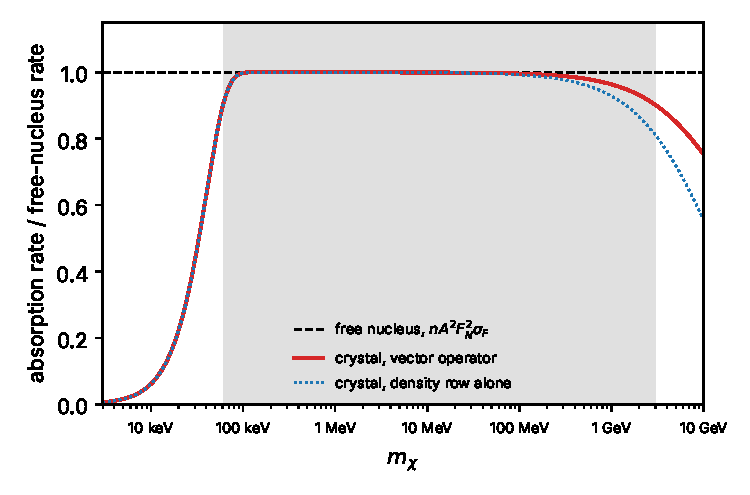
\includegraphics[width=\linewidth]{figures/ch11/limit11_4b.pdf}
\captionof{figure}{Absorption rate of a fermion on silicon nuclei, divided by the free-nucleus rate of the limit check, against $\mchi$, with the nuclear form factor divided out of both. Solid: the vector operator in the crystal, $[1 - \ee^{-2W_\kappa(q_{\mathrm{abs}})}]/(1 + q_{\mathrm{abs}}/M)$ from \cref{eq:11.4-ferm-nuc}, incoherent approximation at $T = 0$ with $\langle u_x^2\rangle = \SI{2.45e-3}{\angstrom^2}$ from the PBE density of states of \cref{sec:5.2}. Dotted: the density row alone, as for the scalar operator, with the recoil factor $(1 - \mchi/M)^2$ to leading order instead of $1 - \mchi/M$. Gray band: $\SI{61}{keV} \le \mchi \le \SI{3.0}{GeV}$, where the vector rate is within \SI{10}{\percent} of the free one.}\label{fig:11-limit-4b}
\par}
\smallskip
Below about \SI{60}{keV} in silicon the absorption must create phonons and the free-nucleus rate overcounts it by $\ee^{-2W_\kappa}/(1 - \ee^{-2W_\kappa})$; above a few GeV the recoil factor $1 - \mchi/M$ and the form factor at $q_{\mathrm{abs}}$ instead of $\mchi$ matter.
\end{limitbox}

\noindent On the truncation label the limit check sits at $n_B = 0$ and $n_T = 0$, with $\mathcal{K}$ = multiphonon (incoherent, all orders) below the impulse onset and $\mathcal{K}$ = impulse above it.

\section{Anharmonic and quantum-crystal corrections}\label{sec:11.5}

At its zero-point amplitude the cubic term of the silicon energy surface is \SI{5}{\percent} of the harmonic one ($\eta_{\mathrm{anh}} = 0.049$, \cref{sec:5.7}), and every formula of \cref{sec:11.3,sec:11.4} dropped it. How much does that change a rate? For the impulse peak, by a part in a thousand. For a deposit of several phonons at a momentum transfer of a few keV, by factors of several, because an anharmonic lattice can make many phonons out of one kick, which a harmonic lattice can only do with many kicks. In solid helium the zero-point motion of an atom is a quarter of the distance to its neighbor, and some harmonic frequencies are imaginary. And in a crystal with a soft mode or a light atom no expansion is available at all, and only exact moments of the response, which anharmonicity cannot change, bound it.

\subsection{Exact moments of the self response}

Above a few zone momenta each nucleus responds on its own (\cref{sec:11.3}), and its self response is controlled by the kick operator $D = E_R + \vect{q}\cdot\vect{p}/M_\kappa$ of \cref{sec:11.4}: the Hamiltonian after the kick is $H + D$, exactly, whatever the potential, provided it depends on the positions of the nuclei and not on their momenta (\cref{eq:D.32-I}). Normalize the response to a distribution in $\omega$, $\dd P = S\,\dd\omega/\int S\,\dd\omega$, with moments $\mu_k = \int\omega^k\,\dd P$ and central moments $\bar\mu_k$, as in \cref{app:C.10}. At $T = 0$, writing $A = H - E_0$, which annihilates the ground state, and $\delta D = D - E_R = (q/M_\kappa)p_{\hat q}$, the central moments are $\bar\mu_k = \langle(A + \delta D)^k\rangle$. Every term with $A$ at either end vanishes. The zeroth moment is $\mu_0 = 1$: the weight of the self response is the norm of $\ee^{\ii\vect{q}\cdot\vect{X}}|0\rangle$. The first is $\mu_1 = E_R$, the sum rule \cref{eq:5.6-sum}. The second and third were derived in \cref{app:D.32}. The fourth needs one more step: of the four terms of $\langle\delta D(A + \delta D)^2\delta D\rangle$, the term $\langle\delta D\,A^2\,\delta D\rangle$ is the squared norm of $A\,\delta D|0\rangle = [H, \delta D]|0\rangle$, and $[H, p_{\hat q}] = \ii\,\partial_{\hat q}V$ is the force along $\hat{\vect{q}}$. The two mixed terms $\langle\delta D\,A\,\delta D^2\rangle$ and its complex conjugate equal $\ii(q/M_\kappa)^3\langle p_{\hat q}(p_{\hat q}\partial_{\hat q}V + \partial_{\hat q}V\,p_{\hat q})\rangle$, by $[H, p_{\hat q}^2] = \ii(p_{\hat q}\partial_{\hat q}V + \partial_{\hat q}V\,p_{\hat q})$; for a real ground-state wavefunction the average is real, so the term is imaginary and cancels against its conjugate. Collecting,
\begin{keyresult}[Exact moments of the self response]
\begin{equation}
  \begin{gathered}
  \mu_0 = 1 , \qquad \mu_1 = E_R , \qquad
  \bar\mu_2 = 4E_RE^{\mathrm{kin}}_\kappa , \\
  \bar\mu_3 = \frac{q^2}{2M_\kappa^2}\bigl\langle\partial_{\hat q}^2V\bigr\rangle , \quad
  \bar\mu_4 = \frac{q^2}{M_\kappa^2}\bigl\langle(\partial_{\hat q}V)^2\bigr\rangle + \frac{q^4}{M_\kappa^4}\bigl\langle p_{\hat q}^4\bigr\rangle ,
  \end{gathered}
  \label{eq:11.5-moments}
\end{equation}
for any potential $V$ of the nuclei, with $E^{\mathrm{kin}}_\kappa = \langle p_{\hat q}^2\rangle/2M_\kappa$ the kinetic energy along $\hat{\vect{q}}$ of \cref{eq:11.4-width}. The averages are over the ground state at $T = 0$; all five moments hold at any temperature with thermal averages (\cref{app:D.32}).
\end{keyresult}
\noindent Each moment is an equal-time average in the ground state: the kinetic energy, the mean curvature of the energy surface, the mean-square force and the fourth moment of the momentum distribution. For a harmonic crystal they reproduce the cumulants of \cref{eq:D.32-ck}; for one oscillator of frequency $\omega_0$, for instance, the mean-square force is $M_\kappa^2\omega_0^4\langle u_{\hat q}^2\rangle = M_\kappa\omega_0^3/2$, so the first term of $\bar\mu_4$ is the fourth cumulant $E_R\omega_0^3$, and the second is $3\bar\mu_2^2$. In an anharmonic crystal the same averages come from a path-integral simulation of the nuclei, which needs no dynamics (\cref{app:E.19}). They are the self part of the moments $\mathscr{M}^k$ of \cref{eq:8.3-moments} for one species, divided by $\mathscr{M}^0$.

Write its relative correction to the harmonic self response as $\delta_{\mathrm{anh}}(\vect{q},\omega) = S_A/S_A^{\mathrm{harm}} - 1$. Then the weight $\int S_A^{\mathrm{harm}}\delta_{\mathrm{anh}}\,\dd\omega$ and the first moment $\int\omega\,S_A^{\mathrm{harm}}\delta_{\mathrm{anh}}\,\dd\omega$ vanish exactly, and the second moment $\int\omega^2S_A^{\mathrm{harm}}\delta_{\mathrm{anh}}\,\dd\omega$ is fixed by the change of the kinetic energy, $4E_R(E^{\mathrm{kin}}_\kappa - E^{\mathrm{kin,harm}}_\kappa)$ times the weight. These three linear constraints test any calculation of the anharmonic response. Time reversal adds a selection rule. For a target invariant under time reversal the eigenfunctions are real, $|\langle f|\ee^{\ii\vect{q}\cdot\vect{X}}|0\rangle|^2 = |\langle f|\ee^{-\ii\vect{q}\cdot\vect{X}}|0\rangle|^2$, and the response is even in $\vect{q}$. A term of first order in $\Phi^{(3)}$ carries three displacements from the cubic term of \cref{eq:5.7-H3}, so it needs an odd number of displacements from the kick to pair them all, and it is odd in $\vect{q}$. It therefore vanishes. The first anharmonic correction to the rate is of second order in $\Phi^{(3)}$ and first order in $\Phi^{(4)}$, the level $n_A = 2$ of \cref{sec:8.5}, of relative size $\eta_{\mathrm{anh}}^2$ by \cref{eq:5.7-order}.

\subsection{Cubic phonon decay}

In the impulse regime the first correction is small. The impulse response \cref{eq:11.4-IA} depends on the potential only through the momentum distribution $\mathfrak{f}_\kappa$, and its width through $E^{\mathrm{kin}}_\kappa$. A single-site model holds the neighbors of one nucleus fixed and gives it a one-dimensional anharmonic potential~\cite[Eq.~(26)]{lin2024anharmonic},
\begin{equation}
  V(x) = \tfrac12M_\kappa\omega_0^2x^2 + \lambda_3\,\omega_0\Bigl(\frac{x}{\ell_0}\Bigr)^3 + \lambda_4\,\omega_0\Bigl(\frac{x}{\ell_0}\Bigr)^4 , \qquad \ell_0 = (2M_\kappa\omega_0)^{-1/2} ,
  \label{eq:11.5-toy}
\end{equation}
with $\ell_0$ the zero-point amplitude of the oscillator. In this potential the cubic energy at $x = \ell_0$ is $4\lambda_3$ times the harmonic one, and $4\lambda_3$ is the anharmonic parameter of \cref{eq:5.7-eta} measured on the site coordinate instead of the bond. Fits of an empirical silicon potential along the bond and perpendicular to it give $\lambda_3 = 0.006$ to $0.01$ and $\lambda_4 = (2$ to $3)\times10^{-4}$~\cite[Sect.~IV]{lin2024anharmonic}, so $4\lambda_3 = 0.024$ to $0.04$, of the size of the bond value $0.049$ of \cref{sec:5.7}. To second order in $\lambda_3$ and first in $\lambda_4$ the kinetic energy becomes $E^{\mathrm{kin}} = (\omega_0/4)(1 - 44\lambda_3^2 + 12\lambda_4)$~\cite[Eq.~(65)]{lin2024anharmonic}, a change within $\pm\SI{0.2}{\percent}$ over the silicon ranges of $\lambda_3$ and $\lambda_4$. The impulse width $\sigma_\omega \propto (E^{\mathrm{kin}})^{1/2}$ then moves by at most a part in a thousand, \SI{0.09}{meV} of the \SI{88}{meV} of \cref{we:11-width}.

At smaller $q$ the correction is of a different kind, because anharmonicity changes how many kicks a given number of phonons needs. Expand the self response of \cref{eq:11.3-exact} in powers of $q$. At $\omega \neq 0$ the constant and the averages of single displacements contribute only at $\omega = 0$, and the first term is the correlation of two displacements,
\begin{equation*}
  S_A(\vect{q},\omega) = \frac{1}{\Omega}\sum_\kappa c_\kappa^2\,q_\alpha q_\beta\int\dd t\;\ee^{\ii\omega t}\bigl\langle u^\alpha_{\kappa}(t)\,u^\beta_{\kappa}(0)\bigr\rangle + O(q^4) ,
\end{equation*}
exact for any anharmonicity. Insert the displacement in phonon coordinates, $\vect{u}_{\vect{R}\kappa} = \sum_{\vect{Q}\nu}(2NM_\kappa\omega_{\vect{Q}\nu})^{-1/2}\vect{e}_{\kappa\nu}(\vect{Q})\ee^{\ii\vect{Q}\cdot\vect{R}}B_{\vect{Q}\nu}$ (\cref{sec:5.3}). The correlation of $B_{\vect{Q}\nu}$ is the spectral function of the dressed propagator $\mathsf{D}_\nu(\vect{Q},\omega) = 2\omega_{\vect{Q}\nu}/[\omega^2 - \omega_{\vect{Q}\nu}^2 - \Pi_\nu(\vect{Q},\omega)]$ of \cref{eq:6.4-Pi}: at $T = 0$ and $\omega > 0$, $\int\dd t\,\ee^{\ii\omega t}\langle B_{\vect{Q}\nu}(t)B_{-\vect{Q}\nu}\rangle = -2\Imag\mathsf{D}_\nu(\vect{Q},\omega)$, which is $2\pi\delta(\omega - \omega_{\vect{Q}\nu})$ for the free phonon. Here $\Pi_\nu$ is the anharmonic self-energy: the bubble of two cubic vertices of \cref{eq:5.7-V3}, whose imaginary part on shell is $-\omega_{\vect{Q}\nu}\gamma^{\mathrm{anh}}_{\vect{Q}\nu}$ (\cref{eq:5.7-gamma,eq:6.4-pole}), and the loop of one quartic vertex, which is real. Off shell, $-\Imag\Pi_\nu(\vect{Q},\omega) = \omega_{\vect{Q}\nu}\gamma^{\mathrm{anh}}_{\vect{Q}\nu}(\omega)$, with $\gamma^{\mathrm{anh}}_{\vect{Q}\nu}(\omega)$ the width of \cref{eq:5.7-gamma} with the energy $\omega$ in place of $\omega_{\vect{Q}\nu}$ in the delta function of the decay: the rate at which a phonon of momentum $\vect{Q}$, given the energy $\omega$, decays into two. With the branches kept separate, as in \cref{sec:6.4}, the harmonic term gives back the one-phonon response \cref{eq:11.1-S1}, a delta function on each branch. Away from the poles, above the one-phonon band, the first order in $\Pi_\nu$ is $-\Imag\mathsf{D}_\nu = 2\omega_{\vect{Q}\nu}(-\Imag\Pi_\nu)/(\omega^2 - \omega_{\vect{Q}\nu}^2)^2$, and
\begin{keyresult}[First anharmonic correction to the nuclear response]
\begin{equation}
  S_A^{\mathrm{anh}}(\vect{q},\omega) = \frac{2\pi}{\Omega}\sum_\kappa c_\kappa^2\,\ee^{-2W_\kappa}\,\frac1N\sum_{\vect{Q}\nu}\frac{|\vect{q}\cdot\vect{e}_{\kappa\nu}(\vect{Q})|^2}{\pi M_\kappa}\;
  \frac{\omega_{\vect{Q}\nu}\,\gamma^{\mathrm{anh}}_{\vect{Q}\nu}(\omega)}{(\omega^2 - \omega_{\vect{Q}\nu}^2)^2} ,
  \label{eq:11.5-anh}
\end{equation}
at $T = 0$, for $\omega$ outside the one-phonon band and $q$ above a few $q_{\mathrm{BZ}}$, where the self part is the response. It is of order $q^2$ and of second order in $\Phi^{(3)}$; the Debye--Waller factor, which the higher orders in $q$ supply, is written to leading order in $\eta_{\mathrm{anh}}$.
\end{keyresult}
\noindent The physical picture is that of \cref{fig:6-bubble} with the electron bubble replaced by a pair of phonons: the kick creates one phonon off its energy shell, and it decays into two real ones. Near $\omega = \omega_{\vect{Q}\nu}$ the same expression, resummed, is the Lorentzian tail of a phonon line of full width $\gamma^{\mathrm{anh}}_{\vect{Q}\nu}$. The two time orderings, the decay of a virtual phonon and the creation of three from the vacuum, have the denominators $1/(\omega - \omega_{\vect{Q}\nu})$ and $1/(\omega + \omega_{\vect{Q}\nu})$, which combine into the $2\omega_{\vect{Q}\nu}/(\omega^2 - \omega_{\vect{Q}\nu}^2)$ of $\mathsf{D}_\nu$.

How large is \cref{eq:11.5-anh} against the harmonic two-phonon response? The harmonic term needs two kicks and carries $q^4$; the anharmonic term needs one kick and the factor $\gamma^{\mathrm{anh}}/\omega \sim \eta_{\mathrm{anh}}^2$. Their ratio is $\sim\eta_{\mathrm{anh}}^2\,2M_\kappa\omega/q^2$, large at small $q$. The model \cref{eq:11.5-toy} makes the counting exact. To first order in $\lambda_3$, with $x/\ell_0 = a + a^\dagger$ and the harmonic states $|n\rangle$ in units of $\omega_0$, the ground state and the second level become
\begin{equation*}
  |\tilde0\rangle = |0\rangle - \lambda_3\Bigl(3|1\rangle + \sqrt{\tfrac23}\,|3\rangle\Bigr) , \qquad
  |\tilde2\rangle = |2\rangle + 6\sqrt2\,\lambda_3|1\rangle + \dots ,
\end{equation*}
where the dots stand for $|3\rangle$ and $|5\rangle$, which the kick does not connect to $|\tilde0\rangle$ at first order in $q$. The coefficient $6\sqrt2$ is $\langle1|(a + a^\dagger)^3|2\rangle$ divided by the level spacing. With $k = q\ell_0$ the kick is $\ee^{\ii k(a + a^\dagger)} = 1 + \ii k(a + a^\dagger) - \frac12k^2(a + a^\dagger)^2 + \dots$. The constant term vanishes between orthogonal states. The linear term gives $\langle\tilde2|a + a^\dagger|\tilde0\rangle = -\lambda_3(3\sqrt2 + \sqrt2) + 6\sqrt2\,\lambda_3 = 2\sqrt2\,\lambda_3$. The quadratic term gives the harmonic $-k^2/\sqrt2$. One amplitude is imaginary and the other real; they do not interfere, and the weight of the second level is
\begin{equation}
  |\langle\tilde2|\ee^{\ii qx}|\tilde0\rangle|^2 = \ee^{-k^2}\Bigl(\frac{k^4}{2} + 8\lambda_3^2k^2 + \dots\Bigr) , \qquad
  \frac{\text{anharmonic}}{\text{harmonic}} = \frac{16\lambda_3^2}{k^2} ,
  \label{eq:11.5-two}
\end{equation}
The anharmonic term wins below $k = 4\lambda_3$, that is, below $q_\times = 4\lambda_3(2M_\kappa\omega_0)^{1/2}$: the crossover sits where the momentum transfer, in units of the inverse zero-point amplitude, equals the anharmonic parameter. For silicon, with $\omega_0 = \langle\omega^{-1}\rangle^{-1} = \SI{30.4}{meV}$, $(2M_\kappa\omega_0)^{1/2} = \SI{39.9}{keV}$ and $q_\times = \SI{1.6}{keV}$ for $\lambda_3 = 0.01$, just below $q_{\mathrm{BZ}} = \SI{2.25}{keV}$. At $q_{\mathrm{BZ}}$ the two-phonon weight is raised by \SI{50}{\percent} for $\lambda_3 = 0.01$ and by \SI{18}{\percent} for $0.006$.

More phonons need more kicks, and the anharmonic gain grows with their number. Three phonons need three kicks in the harmonic crystal, $k^6/6$, but only two with one cubic vertex. That two-kick amplitude alone gives $24\lambda_3^2k^4$; interference between the one-kick amplitude of order $\lambda_3^2k$ and the harmonic three-kick amplitude $k^3/\sqrt6$ subtracts $6\lambda_3^2k^4$, for a net $18\lambda_3^2k^4$. The ratio is then $108\lambda_3^2/k^2$ and the crossover lies at $k = 10.4\lambda_3$, \SI{4.2}{keV} for $\lambda_3 = 0.01$. In general an $n$-phonon weight acquires terms $\lambda_3^{j}k^{2i}$ with $i < n$, and the smaller $i$ the higher the power $j$~\cite[Eqs.~(39), (45)--(48)]{lin2024anharmonic}. \Cref{lim:11.5a} shows the result: for $\lambda_3 = 0.01$ the harmonic two-, three- and four-phonon weights hold within \SI{10}{\percent} only above 5, 12 and \SI{20}{keV}, while at $q_{\mathrm{BZ}}$ the four-phonon weight is 27 times the harmonic one. Which rates does this affect? A threshold of $\omega_{\mathrm{th}}$ needs at least $\omega_{\mathrm{th}}/\omega_{\mathrm{max}}$ phonons, and a particle of mass $\mchi$ reaches at most $q = 2\mchi v_{\mathrm{max}}$. High thresholds and masses of a few MeV are therefore where the harmonic multiphonon rate fails. In the single-site model the anharmonic rate exceeds the harmonic one by up to two orders of magnitude for masses of a few MeV and thresholds of a few phonon energies, in the tail of the spectrum where the rate is small, and the two agree above \SI{10}{MeV}~\cite[Sect.~IV\,A]{lin2024anharmonic}. The anharmonic rate is never below the harmonic one there, because the term of lowest order in $q$ is a square, $|\langle f|\ii qx|\tilde0\rangle|^2$, which the harmonic crystal lacks for $n \ge 2$; this holds for the leading term, not for the full response.

\begin{limitbox}[Anharmonic corrections to multiphonon weights][lim:11.5a]
For a nucleus in the potential \cref{eq:11.5-toy}, the $n$-phonon weight carries, besides the harmonic $\ee^{-k^2}k^{2n}/n!$, terms $\lambda_3^jk^{2i}$ with $i < n$, which dominate for small $k = q\ell_0$; the kinetic energy changes as $1 - 44\lambda_3^2 + 12\lambda_4$~\cite[Eqs.~(39), (45)--(48), (65)]{lin2024anharmonic}.
\par\smallskip
{\centering
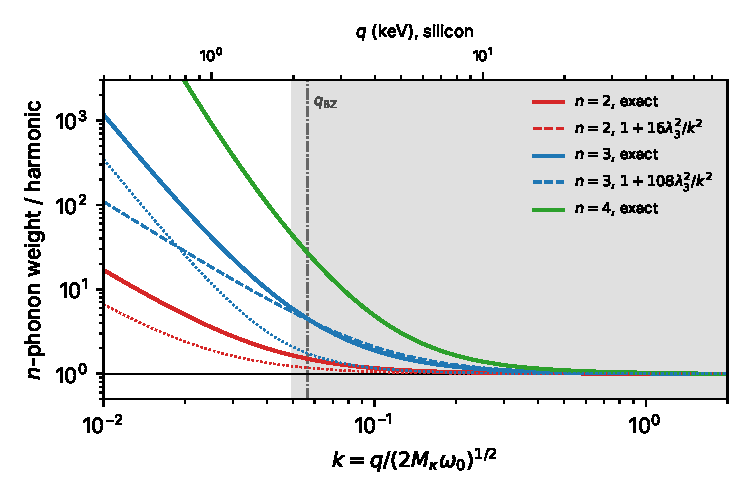
\includegraphics[width=\linewidth]{figures/ch11/limit11_5a.pdf}
\captionof{figure}{Weight of the $n$-th level of the single-site model \cref{eq:11.5-toy}, divided by the harmonic Poisson weight $\ee^{-k^2}k^{2n}/n!$, against $k = q/(2M_\kappa\omega_0)^{1/2}$, for $n = 2$ (red), 3 (blue) and 4 (green). Model with the silicon values $\omega_0 = \SI{30.4}{meV}$, $M_\kappa = \SI{26.16}{GeV}$, $\lambda_3 = 0.01$, $\lambda_4 = 2.5\times10^{-4}$ (solid), and $\lambda_3 = 0.006$, $\lambda_4 = 2\times10^{-4}$ (dotted), solved exactly in 200 oscillator states. Dashed: the leading anharmonic terms, $1 + 16\lambda_3^2/k^2$ for $n = 2$ (\cref{eq:11.5-two}) and $1 + 108\lambda_3^2/k^2$ for $n = 3$. Dash-dotted: $q_{\mathrm{BZ}} = \SI{2.25}{keV}$. Gray band: $k \ge 0.05$, where both leading terms are within \SI{10}{\percent} of the exact weights; below it the three-phonon weight is dominated by a term of order $\lambda_3^4k^2$.}\label{fig:11-limit-5a}
\par}
\smallskip
The model fixes the neighbors, so it overstates the effect below $q_{\mathrm{BZ}}$, where translation invariance makes every multiphonon term of a mass-proportional coupling of order $q^4$; at large $k$ the weights return to the harmonic ones.
\end{limitbox}

\noindent The single-site model breaks translation invariance: a nucleus pulled against fixed neighbors feels a force even when the whole crystal moves. In the real crystal the soft acoustic limit \cref{eq:8.3-soft} is exact, anharmonic terms included, and for a coupling proportional to mass every response at fixed $\omega \neq 0$ vanishes as $q^4$ for $q \ll q_{\mathrm{BZ}}$. The term of order $q^2$ in \cref{eq:11.5-anh} survives because, above $q_{\mathrm{BZ}}$, the self part no longer cancels against the distinct part. Below $q_{\mathrm{BZ}}$ the anharmonic two-phonon response has the same $q^4$ as the harmonic one, and in GaAs it dominates the harmonic term near the on-shell longitudinal-acoustic resonance, where that resonance is kinematically accessible~\cite[Fig.~2]{campbelldeem2020multiphonon}. The window in which the anharmonic $q^2$ term dominates is therefore $q_{\mathrm{BZ}} \lesssim q \lesssim q_\times(n)$, open for three and more phonons in silicon and germanium.

On the truncation label of \cref{sec:8.5}, \cref{eq:11.5-anh} is the first correction along the anharmonic axis, $n_A = 2$, with $\mathcal{K}$ = multiphonon, $n_B = 0$ and $n_T = 0$; at finite temperature the factor $1 + n_B(\omega)$ multiplies it and the thermal factors of \cref{eq:5.7-gamma} enter $\gamma^{\mathrm{anh}}$. The self-energy needs the cubic force constants of the whole crystal on a grid of $\vect{Q}$, which density-functional perturbation theory or finite displacements in a supercell provide (\cref{sec:5.4,app:E.8}). No such calculation exists yet; the single-site model is the only estimate.

\subsection{The Markov--Krein band}

Perturbation theory in $\Phi^{(3)}$ fails for soft modes, light atoms and quantum crystals, but the moments \cref{eq:11.5-moments} do not need it. They are static averages, computable for any anharmonicity, and \cref{app:C.10} shows how much five moments say about a distribution. Every distribution with the moments $\mu_0, \dots, \mu_4$ has its cumulative $F(\xi) = \int_{-\infty}^{\xi}\dd P$ inside the Markov--Krein band \cref{eq:C.10-band}. At each $\xi$ the band is spanned by the canonical representation through $\xi$: three point masses $w_i$ at $y_i$, one of them at $\xi$, that reproduce the five moments, $\sum_iw_iy_i^k = \mu_k$ for $k = 0, \dots, 4$. These are five equations for the two free positions and the three weights. The weight below $\xi$ and the weight up to and including $\xi$ bound $F(\xi)$ from below and above. The width of the band is the mass at $\xi$, the largest that any distribution with these moments can put there: the Christoffel function $\varrho_{\mathrm{MK}}(\xi)$ of \cref{eq:C.10-rho}. For a Gaussian the width is $2/(3 + \xi^4)$, with $\xi$ in standard deviations from the mean (\cref{eq:C.10-gauss}).

\Cref{fig:11-mk} draws the band around the harmonic response of silicon at $q = \SI{100}{keV}$, the momentum of \cref{we:11-width}, and at \SI{50}{keV}. The moments are those of the cumulants $c_k = E_R\langle\omega^{k-1}\rangle$ of \cref{eq:D.32-ck}, which the numerical spectrum reproduces to $10^{-6}$ at \SI{100}{keV}. The response lies inside the band everywhere, as it must. Near the peak the band is wide (\cref{we:11-mkpeak}); at \SI{50}{keV}, where the zero-phonon line puts a step of 0.21 at $\omega = 0$ and the phonon bands show, it spans 0.21 to 0.89 at $\omega = E_R$. In the tails it narrows as $(\xi - \mu_1)^{-4}$, with the coefficient $\bar\mu_4 - \bar\mu_2^2 - \bar\mu_3^2/\bar\mu_2$ of \cref{eq:C.10-tail}.

\begin{figure}[tbp]
  \centering
  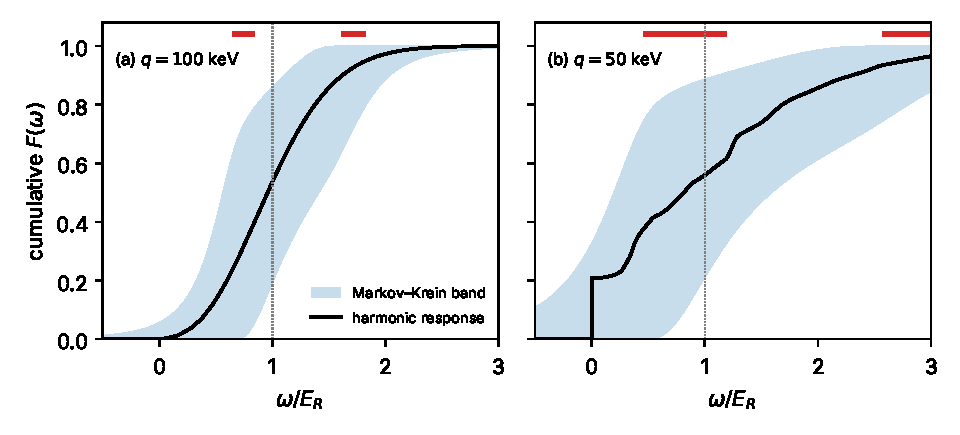
\includegraphics[width=\linewidth]{figures/ch11/fig11_5.pdf}
  \caption{Cumulative nuclear response $F(\omega)$ of silicon at $T = 0$ (black), the fraction of the weight of the self response at energies up to $\omega$, against $\omega/E_R$, with the Markov--Krein band of its first five moments (blue). (a)~$q = \SI{100}{keV}$, $E_R = \SI{191.1}{meV}$, $x_R = 4.67$; (b)~$q = \SI{50}{keV}$, $E_R = \SI{47.8}{meV}$, $x_R = 1.17$, where the zero-phonon weight $\ee^{-2W_\kappa} = 0.21$ is a step at $\omega = 0$. Response: harmonic, incoherent, all phonon orders, from the PBE density of states of \cref{sec:5.2}; moments from $c_k = E_R\langle\omega^{k-1}\rangle$. Red bars: values of $\omega$ at which a node of the canonical representation lies below $\omega = 0$, so that the band drawn is wider than the sharp band of distributions confined to $\omega \ge 0$; elsewhere it is sharp for them too. Dotted: $\omega = E_R$.}
  \label{fig:11-mk}
\end{figure}

At $T = 0$ the response vanishes for $\omega < 0$, a constraint that the band of \cref{eq:C.10-band} does not use. It remains valid, and where every node of the canonical representation lies at $\omega \ge 0$ that representation is itself an admissible response, which makes the band sharp on the half line too. This holds at $\omega = E_R$ for $q = \SI{100}{keV}$ (\cref{we:11-mkpeak}). It fails in two windows, $0.65$ to $0.85\,E_R$ and $1.61$ to $1.82\,E_R$, where one outer node of the three-point solution moves out to infinity and comes back from the other side, below $\omega = 0$; at \SI{50}{keV} the windows are $0.46$ to $1.20\,E_R$ and $2.6$ to $3.4\,E_R$. There the half-line point-mass bound \cref{eq:C.10-stieltjes} is smaller than $\varrho_{\mathrm{MK}}$, by up to \SI{6.8}{\percent} at \SI{100}{keV} and \SI{24.5}{\percent} at \SI{50}{keV}, so the sharp half-line band is narrower at least by that much. We use the band \cref{eq:C.10-band} throughout, which is conservative and has explicit extremal distributions.

\begin{workedexample}{Markov--Krein band of silicon at the recoil energy}\label{we:11-mkpeak}
Take silicon at $q = \SI{100}{keV}$ and $T = 0$, with $E_R = \SI{191.1}{meV}$ and $\langle\omega\rangle = \SI{40.9}{meV}$ as in \cref{we:11-width}. The cumulants $c_k = E_R\langle\omega^{k-1}\rangle$ give the standard deviation $\sigma_\omega = \SI{88.4}{meV}$, the skewness $c_3/\sigma_\omega^3 = 0.553$ and the standardized fourth moment $3 + c_4/c_2^2 = 3 + (\langle\omega^3\rangle/\langle\omega\rangle^3)/x_R = 3.333$, against 0 and 3 for a Gaussian. For a Gaussian the canonical representation through the mean has nodes at 0 and $\pm\sqrt3$ standard deviations with weights $\tfrac23, \tfrac16, \tfrac16$ (\cref{app:C.10}). For silicon the same construction, \cref{eq:C.10-kernel} with these moments, puts the nodes at 59.8, 191.1 and \SI{371.3}{meV} with weights 0.191, 0.670 and 0.139. The skewness pushes the outer nodes upward and moves weight to the lower one, but leaves the central weight at $\varrho_{\mathrm{MK}}(E_R) = 0.670$, almost the Gaussian 2/3. So
\begin{equation*}
  0.191 \le F(E_R) \le 0.861 ,
\end{equation*}
while the harmonic response has $F(E_R) = 0.537$. A detector with its threshold at $E_R$ sees between 14 and \SI{81}{\percent} of the events of this momentum transfer, whatever the dynamics, if only the five moments are right.

Energy bins narrow the band little. Between $E_R - \sigma_\omega$ and $E_R + \sigma_\omega$ the band allows any weight from 0.07 to 1.00 (the harmonic value is 0.68); between $E_R \pm 2\sigma_\omega$ it allows 0.78 to 1.00 (0.96). In the tail it is worse in relative terms: above $E_R + 3\sigma_\omega = \SI{456}{meV}$ the harmonic response has the weight $5.6\times10^{-3}$, and the band allows anything from 0 to $3.4\times10^{-2}$, six times more.

The anharmonic change of the kinetic energy of silicon moves the cumulative distribution by at most $2.5\times10^{-4}$, nearly three thousand times less than the width of the band at the peak. For silicon the perturbative correction of the previous subsection is the tool; the band is for targets where no correction can be computed.
\end{workedexample}

In silicon at \SI{100}{keV} the band fixes the weight above a threshold to \SI{10}{\percent} only for thresholds at $\omega \le \SI{28}{meV}$ (\cref{lim:11.5c}). At five standard deviations above the mean the band is 63 times the weight.

\begin{limitbox}[The Markov--Krein band][lim:11.5c]
Every distribution with the moments $\mu_0, \dots, \mu_4$ has $\sum_{y_i < \xi}w_i \le F(\xi) \le \sum_{y_i \le \xi}w_i$, of width $\varrho_{\mathrm{MK}}(\xi)$, with $(y_i, w_i)$ the canonical representation through $\xi$; far from the mean $\varrho_{\mathrm{MK}} \simeq (\bar\mu_4 - \bar\mu_2^2 - \bar\mu_3^2/\bar\mu_2)/(\xi - \mu_1)^4$~\cites{krein1977markov}{akhiezer1965classical}.
\par\smallskip
{\centering
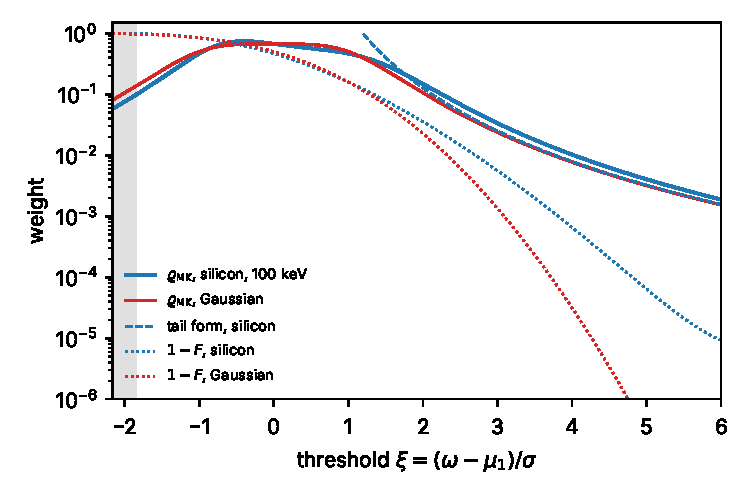
\includegraphics[width=\linewidth]{figures/ch11/limit11_5c.pdf}
\captionof{figure}{Width $\varrho_{\mathrm{MK}}$ of the band (solid) and weight $1 - F$ above a threshold (dotted), against the threshold $\xi$ in units of the standard deviation from the mean, for the harmonic silicon response at $q = \SI{100}{keV}$ (blue; skewness 0.553, standardized fourth moment 3.333) and for a Gaussian (red), the two model distributions whose five moments define their bands. Dashed: the tail form \cref{eq:C.10-tail} for silicon, the leading term far from the mean, with the numerator 2.03 (2 for the Gaussian); the exact width exceeds it by \SI{34}{\percent} at $\xi = 3$ and \SI{20}{\percent} at $\xi = 6$, a correction of relative order $1/\xi$ from the skewness. The silicon curves start at $\omega = 0$. Gray band: thresholds at which the band fixes the silicon weight above threshold to \SI{10}{\percent}, $\varrho_{\mathrm{MK}} \le 0.1\,(1 - F)$, that is $\xi \le -1.84$.}\label{fig:11-limit-5c}
\par}
\smallskip
Above about two standard deviations below the mean the absolute width exceeds a tenth of the weight above threshold, and in the tail it exceeds the weight itself: the band bounds the bulk of a response, never the ratio of two tails.
\end{limitbox}

\noindent On the truncation label the band is exact in $n_A$ and in $n_T$ when the moments are, and it makes no assumption about $\mathcal{K}$. Its use is twofold. For a strongly anharmonic target at a detector temperature it is the only rigorous statement about the response, since the moments come from a static simulation and every real-time method has a problem at millikelvin (below). And for any approximate dynamics it is an acceptance test: a computed response outside the band of its exact moments is wrong.

\subsection{Solid helium}

Helium solidifies only under a pressure of a few MPa even at the lowest temperatures~\cite{ashour2024pressure}, because the zero-point energy of so light an atom in so shallow a well, \SI{10.8}{K} deep for a pair~\cite{aziz1979accurate}, competes with the binding itself. Such a solid is a \emph{quantum crystal}: the zero-point amplitude of an atom is a sizable fraction of the distance to its neighbors, about a quarter near melting, and the harmonic expansion fails at its lowest order. The Lindemann ratio $r_{\mathrm{L}} = \langle u^2\rangle^{1/2}/d_{\mathrm{nn}}$, the root-mean-square displacement over the nearest-neighbor distance $d_{\mathrm{nn}}$, measures it. At the static lattice positions an atom sits far out on the attractive tail of its neighbors' potentials, where the curvature is negative, and the static force constants give imaginary frequencies. The self-consistent harmonic approximation of \cref{eq:5.7-scha} was devised for this case: averaged over the Gaussian spread of the atom, the curvature includes the steep repulsion that the atom samples on its excursions, and it is positive. Compression reduces $r_{\mathrm{L}}$. Diffusion Monte Carlo calculations with a pair potential fitted to dispersion-corrected density-functional theory find $r_{\mathrm{L}} = 0.12$ at \SI{2}{GPa} and 0.10 from \SI{14}{GPa} up to \SI{150}{GPa}~\cite[Table~I]{cazorla2015first}. At such pressures the static lattice is stable, and the quasi-harmonic approximation of \cref{sec:5.7} becomes a reasonable starting point.

Ashour and Griffin proposed solid helium under pressure as a target for light dark matter that couples to nucleons~\cite{ashour2024pressure}. At low pressure its phonon energies are below \SI{3}{meV} and its sound speed is of order $10^{-6}$, too low for single-phonon reach. Between 1 and \SI{40}{GPa} the sound speed rises more than tenfold and the phonon energies nearly a hundredfold, and at \SI{40}{GPa} the single-phonon reach of hcp helium rivals that of diamond. Their response is that of \cref{lim:11.5b}, with phonons computed with the PBE functional and a dispersion correction, and it leaves out the low pressures, where the density functional fails and the Born--Oppenheimer phonons miss the zero-point motion.

When is the quasi-harmonic response good enough, and what does the self-consistent one add? \Cref{lim:11.5b} answers in a cell model, in which one atom moves in the field of its twelve neighbors held fixed on an fcc lattice and the Schrödinger equation is solved exactly. The pair potential is a Morse form with the well of the helium potential, so that only one shape parameter is chosen (the curvature at the minimum of a 12-6 potential with the same well). The model gives $r_{\mathrm{L}} = 0.23$ at \SI{21}{cm^3.mol^{-1}}, near melting, where its first excitation lies at \SI{2.2}{meV}, and 0.117 and 0.094 at the volumes of the Monte Carlo values 0.12 and 0.10 above. The static curvature turns negative for molar volumes above \SI{17}{cm^3.mol^{-1}}, $r_{\mathrm{L}} \ge 0.20$. Below that the quasi-harmonic weight of a single phonon, $q^2/2M\omega$ per direction, overshoots the exact one, because the static curvature is too soft; the error falls below \SI{10}{\percent} only for $r_{\mathrm{L}} \le 0.115$, a molar volume of \SI{6.5}{cm^3.mol^{-1}}, about the \SI{2}{GPa} of the Monte Carlo calculation. The self-consistent harmonic weight stays within \SI{10}{\percent} up to $r_{\mathrm{L}} = 0.227$ and is \SI{10}{\percent} low at \SI{21}{cm^3.mol^{-1}}. The kinetic energy that sets the impulse width behaves alike: at $r_{\mathrm{L}} = 0.117$ the quasi-harmonic value is \SI{9}{\percent} low and the self-consistent one within \SI{0.1}{\percent}.

\begin{limitbox}[Solid helium: quasi-harmonic and self-consistent phonons][lim:11.5b]
The single-phonon rate of compressed helium is \cref{eq:11.1-S1} with $c_\kappa = A_\kappa F_N$, phonons and Debye--Waller exponent from the static Hessian at the compressed volume~\cite[Eqs.~(2), (4), (5)]{ashour2024pressure}; the self-consistent correction replaces the Hessian by $\Phi^{(2)}_{\mathrm{aux}}$ of \cref{eq:5.7-scha}.
\par\smallskip
{\centering
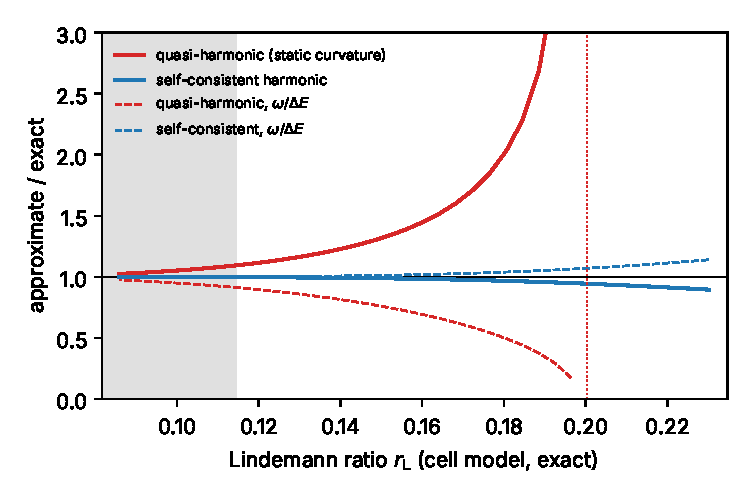
\includegraphics[width=\linewidth]{figures/ch11/limit11_5b.pdf}
\captionof{figure}{Cell model of solid $^4$He: one atom in the spherically averaged field of 12 fixed fcc neighbors, Morse pair potential with the well depth \SI{10.8}{K} and position \SI{2.967}{\angstrom} of the Aziz potential and a curvature equal to that of a 12-6 potential with the same well. Solid: one-phonon weight per unit $q^2$, $1/2M\omega$, from the static curvature (red, quasi-harmonic) and from the self-consistent curvature (blue), divided by the exact dipole weight of the lowest $l = 1$ level, against the exact Lindemann ratio $r_{\mathrm{L}}$, for molar volumes from 3 to \SI{21}{cm^3.mol^{-1}}. Dashed: the corresponding phonon energies over the exact excitation energy $\Delta E$. Dotted: $r_{\mathrm{L}} = 0.20$, above which the static curvature is negative. Gray band: $r_{\mathrm{L}} \le 0.115$, where the quasi-harmonic weight is within \SI{10}{\percent}.}\label{fig:11-limit-5b}
\par}
\smallskip
Above a Lindemann ratio of about 0.12 the static Hessian overstates the one-phonon weight and the Debye--Waller exponent, and above 0.20 it has no real frequencies; the self-consistent phonons hold to near melting, where correlations at short range remain.
\end{limitbox}

\noindent The model fixes the neighbors and uses a Morse wall, so its numbers are a guide, not a prediction for helium; it lands within $0.003$ and $0.006$ of the two Monte Carlo ratios. The quasi-harmonic response of Ashour and Griffin is safe in most of their pressure range and needs the self-consistent force constants at its low end. And at the lowest pressures, where a helium detector would be easiest to build, neither is exact. The self-consistent weight is \SI{10}{\percent} low near melting even in the model, and in the real crystal the Gaussian lets an atom overlap its neighbors, which a real atom avoids by correlated motion. There the response needs the exact moments and the band of \cref{lim:11.5c}. On the truncation label the self-consistent response sums the even anharmonic orders into $\Phi^{(2)}_{\mathrm{aux}}$ at all $n_A$. The cubic terms enter the physical frequencies through a bubble; in the cubic cell of the model the centroid sits on the site and that bubble vanishes.

The same reasoning sorts the other targets in which anharmonicity is not small. A soft mode, such as the one that drives the structural transition of SrTiO$_3$, has a harmonic frequency that is small or imaginary, and its self-consistent frequency depends on temperature at order one. A light atom, such as hydrogen in LiH, has a zero-point amplitude larger by $(M_{\mathrm{Si}}/M_{\mathrm{H}})^{1/4} \approx 2.3$ than a silicon atom in the same well, since $\ell_{\mathrm{zp}} \propto M^{-1/4}$ (\cref{sec:5.7}), and $\eta_{\mathrm{anh}}$ grows with it.

\emph{Open problem: the response of strongly anharmonic targets at detector temperatures.} For soft-mode and light-atom crystals, and for solid helium near melting, no expansion parameter is small, and the nuclear response at \SI{10}{mK} has not been computed. The exact moments are within reach: they are static averages, and a path-integral simulation gives them at any temperature and anharmonicity. The dynamics is not. Ring-polymer and centroid molecular dynamics return Kubo-transformed correlations. Their conversion to $S$ multiplies the error by $\omega/T$, so they hold only for $T \gtrsim \omega/10$; the time-dependent self-consistent harmonic method excites at most two phonons at a time and cannot follow a multiphonon response at $q \gg q_{\mathrm{BZ}}$. At the operating temperature of a cryogenic detector the response of these targets is therefore bounded by the band of their exact moments and by nothing sharper. What would close the gap is a real-time method for quantum nuclei that is exact at low temperature, or a measurement: neutron Compton scattering measures the momentum distribution, and with it the impulse width, of light nuclei directly~\cite{andreani2005measurement}.

\section{Nuclear-spin and isotope couplings}\label{sec:11.6}

One silicon nucleus in 21 is $^{29}$Si and carries a nuclear spin, and in a crystal without a magnetic field the spins point in random directions. The three stable isotopes also differ in their number of neutrons per unit mass, by \SI{6.7}{\percent} from $^{28}$Si to $^{30}$Si. The couplings of \cref{sec:11.1,sec:11.2} are the same on every site of a sublattice, and they conserve crystal momentum. A coupling to the nuclear spin, or to the neutron number of a nucleus at fixed mass, changes at random from site to site. The lattice is still perfect, but to the dark matter the crystal is disordered, crystal momentum is no longer conserved, and a probe that brings almost no momentum, such as an absorbed boson, can create a phonon of any wavevector in the zone. The response then follows the phonon density of states, a broad band, instead of the single line of the zone-center optical phonon. Unpolarized nuclear spins respond in this way, and so do the isotopes to a vector boson coupled to baryon minus lepton number, which in silicon is absorbed almost entirely through them.

\subsection{Broadband response of random couplings}\label{sec:11.6-random}

Label the nuclei of a crystal by $I$, with masses $M_I$ and displacements $\vect{u}_I$ from their equilibrium positions. In a harmonic crystal the displacements are sums over normal modes $\nu$ of the actual configuration, with polarization vectors $\vect{e}_{I\nu}$ normalized over all sites and the mode frequencies $\omega_\nu$, $\vect{u}_I = \sum_\nu\vect{e}_{I\nu}(b_\nu + b_\nu^\dagger)/\sqrt{2M_I\omega_\nu}$. In a perfect crystal $\nu$ is the pair $\vect{Q}\nu$ of \cref{eq:5.3-u}; when the masses vary from site to site, the modes carry no wavevector and $\nu$ is just a label. Consider a target operator whose one-phonon matrix element is linear in the displacements,
\begin{equation*}
  \langle 1_\nu|\,O\,|0\rangle = \sum_I\frac{\vect{v}_I\cdot\vect{e}_{I\nu}^*}{\sqrt{2M_I\omega_\nu}} ,
\end{equation*}
with a vertex $\vect{v}_I$ for each site. The density row at small $\vect{q}$ has this form, with $\vect{v}_I = \ii c_I\vect{q}$ (\cref{sec:11.1}). So has every row built from the nuclear velocities $\vect{P}_I/M_I$. In a harmonic crystal the momentum is $M_I$ times the time derivative of the displacement, and the derivative of a matrix element brings down $\ii\omega$, with $\omega$ the energy of the final state: $\langle f|\vect{P}_I|0\rangle = \ii M_I\omega\langle f|\vect{u}_I|0\rangle$.

Part of every vertex does nothing. Write $\vect{v}_I = M_I\bar{\vect{v}} + \delta\vect{v}_I$ with $\bar{\vect{v}} = \sum_I\vect{v}_I/\sum_IM_I$. The uniform translation of the crystal is a zero mode with $\vect{e}_{I0} \propto \sqrt{M_I}$, every vibration is orthogonal to it, $\sum_I\sqrt{M_I}\,\vect{e}_{I\nu} = 0$, and the mass-proportional part drops out of every one-phonon element. Mitridate and collaborators noted this coupling-to-mass cancellation for the zone-center optical phonons of a perfect crystal~\cite[Eq.~(44)]{mitridate2024effective}. It holds for any configuration of masses, not only at the zone center of a perfect crystal: a coupling proportional to the mass of each nucleus couples to the total momentum, which the forces of the lattice conserve. Only the deviations $\delta\vect{v}_I$ create phonons.

Suppose now that the $\delta\vect{v}_I$ are random: zero on average, independent from site to site and isotropic, $\langle\delta v^\alpha_I\,\delta v^{\beta*}_J\rangle = \delta_{IJ}\delta^{\alpha\beta}\langle|\delta\vect{v}_I|^2\rangle/3$. Averaging the squared matrix element over the disorder removes every term with $I \neq J$, together with the phases that enforced crystal momentum. Each site then contributes through its own vibrations, measured by the local density of states
\begin{equation*}
  g_I(\omega) = \sum_\nu|\vect{e}_{I\nu}|^2\,\delta(\omega - \omega_\nu) ,
\end{equation*}
normalized to three by the completeness of the polarization vectors; in a crystal of one isotope it is the atom-projected density of states $g_{\mathrm{ph},\kappa}$ of \cref{sec:5.3}. Summing over the modes with \cref{eq:4.2-Sab} gives
\begin{keyresult}[Broadband one-phonon response of a random coupling]
\begin{equation}
  \bigl\langle S_{OO}(\vect{q}\to0,\omega)\bigr\rangle = \frac{2\pi}{\Vol}\sum_I\langle|\delta\vect{v}_I|^2\rangle\,\frac{g_I(\omega)}{6M_I\,\omega}\,\bigl[n_{\mathrm{B}}(\omega) + 1\bigr] ,
  \label{eq:11.6-random}
\end{equation}
for $\omega > 0$, with the Bose factor of \cref{sec:5.3} and the average over the disorder in the brackets. It is exact for a harmonic crystal when the random vertex is independent of the masses and force constants, with $g_I$ the local density of states at site $I$ of the actual crystal.
\end{keyresult}
\noindent Unlike the single zone-center line that a coherent coupling excites (\cref{sec:11.2}), the response is a band: every phonon of energy $\omega$ contributes, whatever its wavevector, since the random vertex supplies the missing crystal momentum. And it does not depend on how the vertices of neighboring sites are related, only on the variance at each site. On the truncation label of \cref{sec:8.5} it is the point $\mathcal{K}$ = one-phonon, $n_A = 0$, $n_B = 0$, with $n_T = 0$ at \SI{10}{mK}; the coherent sum of \cref{eq:11.1-S1} is replaced by its incoherent counterpart, and this time without approximation.

\subsection{Unpolarized nuclear spins}\label{sec:11.6-spins}

A coupling linear in the nucleon spin acts on a nucleus of isotope $i$ through its spin $\vect{J}^{\mathrm{nuc}}_I$, with the coefficient of \cref{eq:8.1-nuclear}. It enters the target through the spin rows of \cref{eq:8.1-rows}, the spin density $\vect{s}_\kappa(\vect{q}) = \sum_I\ee^{\ii\vect{q}\cdot\vect{X}_I}\vect{J}^{\mathrm{nuc}}_I$ and the spin current $\mathcal{J}^{\alpha\beta}_\kappa$. In zero field the spin states of a nucleus are split only by its quadrupole and dipolar interactions, by at most about \SI{0.1}{\micro eV}, against $T = \SI{0.86}{\micro eV}$ at \SI{10}{mK}. A spin $\frac12$ such as $^{29}$Si has no quadrupole splitting at all, and its states are equally occupied. A nucleus with a quadrupole moment keeps $\langle\vect{J}^{\mathrm{nuc}}\rangle = 0$ but can be slightly aligned at millikelvin temperatures; we do not pursue this correction. The spins also barely act on the lattice: the forces between the atoms are electronic, and the hyperfine coupling that ties a nuclear spin to anything else is far weaker. The state of the target is then a product of an equal mixture of spin states for each nucleus and the phonon state, and
\begin{equation*}
  \bigl\langle J^{a}_IJ^{b}_{I'}\bigr\rangle = \delta_{II'}\,\delta^{ab}\,\frac{J_{\mathrm{nuc},i}(J_{\mathrm{nuc},i} + 1)}{3} ,
\end{equation*}
with $J_{\mathrm{nuc},i}$ the spin of isotope $i$. Two different nuclei have uncorrelated spins, so in the correlation form of \cref{eq:4.2-Sab} every pair of distinct nuclei drops out of the spin-density response, at every phonon order and every temperature. What remains is the self part of \cref{sec:11.3}, one nucleus at both times, for the nuclei that carry a spin:
\begin{keyresult}[Spin-density response of unpolarized nuclei]
\begin{equation}
  \begin{gathered}
  S_{s^as^b}(\vect{q},\omega) = \delta^{ab}\sum_i\frac{J_{\mathrm{nuc},i}(J_{\mathrm{nuc},i} + 1)}{3}\,S^{\mathrm{self}}_i(\vect{q},\omega) , \\
  S^{\mathrm{self}}_i(\vect{q},\omega) = \frac1\Vol\int_{-\infty}^{\infty}\dd t\;\ee^{\ii\omega t}\sum_{I\in i}\bigl\langle\ee^{-\ii\vect{q}\cdot\vect{X}_I(t)}\,\ee^{\ii\vect{q}\cdot\vect{X}_I(0)}\bigr\rangle ,
  \end{gathered}
  \label{eq:11.6-spinS}
\end{equation}
the sum running over the isotopes with a spin. The self response is \cref{eq:11.3-inc} for these nuclei with $c_\kappa^2 \to 1$; its one-phonon term at $T = 0$ on a cubic site is $(2\pi/\Vol)N_i\,\ee^{-2W_i}\,(q^2/2M_i\omega)\,g_i(\omega)/3$, with $N_i$ the number of nuclei of isotope $i$.
\end{keyresult}
\noindent The incoherent approximation of \cref{sec:11.3}, there valid only far above the zone, is exact here at every momentum transfer. The spin-dependent operator $\mathcal{O}_4 = \vect{S}_\chi\cdot\vect{S}_N$ has the dark-matter tensor $\mathfrak{D}_{s^as^b} = |c_4^{(i)}|^2\delta^{ab}|\vect{S}_\chi|(|\vect{S}_\chi| + 1)/3$ of \cref{eq:8.1-D}, and the contraction in the rate \cref{eq:8.2-spectrum} is $\sum_i|c_4^{(i)}|^2\,|\vect{S}_\chi|(|\vect{S}_\chi| + 1)\,J_{\mathrm{nuc},i}(J_{\mathrm{nuc},i} + 1)\,S^{\mathrm{self}}_i/3$. In silicon only $^{29}$Si contributes, with $J_{\mathrm{nuc}} = \frac12$, an abundance of \SI{4.685}{\percent}, and $c_4^{(i)} = 0.312\,c_4^{(n)}$ for a coupling to neutron spins alone (\cref{sec:8.1-nuclei}).

The loss of crystal momentum changes the kinematics. A coherent one-phonon response at $q \ll q_{\mathrm{BZ}}$ offers only acoustic phonons of energy $c_\nu q$, and the reach stops at the acoustic edge \cref{eq:11.1-edge}. The self response at the same $q$ spans the whole band, and any energy up to the kinetic energy of the dark matter can be deposited. A spin-dependent coupling of unpolarized nuclei therefore reaches down to the kinematic limit $2\omega_{\mathrm{th}}/v_{\mathrm{max}}^2$ of a free target, \cref{eq:1.3-mmin}, \SI{0.28}{keV} at a \SI{1}{meV} threshold, 21 times below the acoustic edge of silicon. The weight, however, is small: the self response grows as $q^2$, and at the smallest momentum transfers it is tiny.

Absorption needs the spin current. An axion-like particle couples to nucleons as to electrons in \cref{sec:1.4}, $\mathcal{L} \supset g_{aNN}\,\phi\,\bar\psi_N\ii\gamma^5\psi_N$ for $N = p, n$, and the reduction that gave \cref{eq:8.1-alp} gives for each nucleon $(g_{aNN}/m_N)[(\nabla\phi)\cdot\vect{S}_N + (\partial_t\phi)\,\vect{v}_N\cdot\vect{S}_N]$, with $\vect{v}_N$ the nucleon velocity. Inside a nucleus the velocity of each nucleon is that of the nucleus, $\vect{P}_I/M_i$, plus an internal part that averages to zero, and the Wigner--Eckart theorem replaces the weighted sum of nucleon spins by $g_{ai}\vect{J}^{\mathrm{nuc}}_I$ with
\begin{equation*}
  g_{ai} = \frac{g_{app}\langle S_p\rangle + g_{ann}\langle S_n\rangle}{J_{\mathrm{nuc},i}} ,
\end{equation*}
as in \cref{eq:8.1-nuclear}. The interaction is then $m_N^{-1}\sum_ig_{ai}[(\nabla\phi)\cdot\vect{s}_i + (\partial_t\phi)\,\mathcal{J}^{\alpha\alpha}_i]$ at $\vect{q} = \vect{p}_\phi$. The gradient term rotates a nuclear spin and leaves the lattice as it was. Its final states lie at the spin splittings, below a \si{\micro eV}, and never at $\omega = m_\phi$; it would excite a phonon only through the phase $\ee^{\ii\vect{p}_\phi\cdot\vect{u}_I}$, a correction of order $p_\phi^2\langle u_x^2\rangle \approx 2\times10^{-18}$ at \SI{50}{meV}. The time-derivative term moves the nucleus. At $\vect{p}_\phi \to 0$ it is exactly linear in the nuclear momenta, $\mathcal{J}^{\alpha\alpha}_i = \sum_{I\in i}\vect{P}_I\cdot\vect{J}^{\mathrm{nuc}}_I/M_i$, so in a harmonic crystal it creates exactly one phonon, with the vertex $\delta\vect{v}_I = \ii\omega\,(g_{ai}m_\phi/m_N)\,\vect{J}^{\mathrm{nuc}}_I$ in \cref{eq:11.6-random}, whose variance over the spin states is $\omega^2(g_{ai}m_\phi/m_N)^2J_{\mathrm{nuc},i}(J_{\mathrm{nuc},i} + 1)$. The absorption formula \cref{eq:8.2-abs} with $\omega_\phi = m_\phi$ and the event rate per unit mass $(\rho_\chi/m_\phi\rho_T)\varGamma_{\mathrm{abs}}$ then give, at $T = 0$,
\begin{equation}
  \mathcal{R} = \frac{\pi\rho_\chi m_\phi}{6\,m_N^2M_{\mathrm{cell}}}\sum_{\kappa}\sum_ix_{\kappa i}\,g_{ai}^2\,\frac{J_{\mathrm{nuc},i}(J_{\mathrm{nuc},i} + 1)}{M_i}\,g_i(m_\phi) ,
  \label{eq:11.6-alp}
\end{equation}
with $x_{\kappa i}$ the abundance of isotope $i$ on the sites $\kappa$ of the cell and $M_{\mathrm{cell}}$ the mass of the cell. The rate is broadband: from the lowest acoustic phonons to the top of the optical band, every axion mass is absorbed at the rate set by the density of states at $\omega = m_\phi$. Per unit mass, light nuclei with a large spin weight are favored through the factor $1/M_iM_{\mathrm{cell}}$. In silicon the spin weight is $x_{29}(0.312)^2\cdot\frac34 = 3.4\times10^{-3}$ in units of $g_{ann}^2$, and the proton coupling enters with a coefficient ten times smaller, through $\langle S_p\rangle = 0.016$. \Cref{eq:11.6-alp} is the rate of Bloch, Knapen, Madden and Marocco~\cite[Eq.~(31)]{bloch2025broadband}, who couple the axion to nucleons through $g_N\partial_\mu\phi\,\bar\psi_N\gamma^\mu\gamma^5\psi_N$. On shell this is our coupling with $g_{aNN} = 2m_Ng_N$, and their $g_p\lambda_j$, $\xi_j$ and $D_j(\omega)$ are our $g_{ai}/2m_N$, the weight $\lambda_j^2J(J+1)/M$ averaged over isotopes, and $g_i/3$.

The spin sits on $^{29}$Si, however, which is \SI{3.2}{\percent} heavier than the mean silicon atom, and its local density of states $g_{29}$ is not the $g_{\mathrm{ph},\kappa}$ of the crystal; the literature uses the host density of states for every isotope.

\subsection{An isotopic mass defect}\label{sec:11.6-defect}

How does a single heavier atom vibrate in a crystal of lighter ones? Its neighbors push it with the same springs, and only its inertia differs. The displacement response of a harmonic crystal, the retarded Green function $\GF(\omega) = (\Phi - \omega^2\mathsf{M} - \ii0)^{-1}$ with $\Phi$ the matrix of force constants of \cref{sec:5.2} and $\mathsf{M}$ the diagonal matrix of masses, answers this. In a crystal of mean mass $\bar M$ the element on one site, for one Cartesian direction, is
\begin{equation*}
  \GF_{\mathrm{h}}(\omega) = \frac{1}{\bar M}\int_0^{\infty}\dd\omega'\,\frac{g_{\mathrm{ph},\kappa}(\omega')/3}{\omega'^2 - \omega^2 - \ii0} , \qquad
  \Imag\GF_{\mathrm{h}}(\omega) = \frac{\pi\,g_{\mathrm{ph},\kappa}(\omega)}{6\bar M\omega} ,
\end{equation*}
the spectral sum over the modes weighted by the squared polarization on the site; on a cubic site it is a multiple of the identity. Now give the atom on site $I$ the mass $M_i = \bar M(1 - \delta^M_i)$, with the mass defect $\delta^M_i$ positive for a lighter atom. The change in $\Phi - \omega^2\mathsf{M}$ is the single entry $\delta^M_i\bar M\omega^2$ on that site, and since it acts on one site only, the Dyson equation $\GF = \GF_{\mathrm{h}} - \GF_{\mathrm{h}}\,\delta^M_i\bar M\omega^2\,\GF$ closes on the element at $I$. The local density of states follows from $\Imag\GF$ as for the host, with $M_i$ for $\bar M$:
\begin{keyresult}[Local vibrations of one mass defect]
\begin{equation}
  \GF_i(\omega) = \frac{\GF_{\mathrm{h}}(\omega)}{1 + \delta^M_i\,\bar M\omega^2\,\GF_{\mathrm{h}}(\omega)} , \qquad
  \frac{g_i(\omega)}{g_{\mathrm{ph},\kappa}(\omega)} = (1 - \delta^M_i)\,\frac{\Imag\GF_i(\omega)}{\Imag\GF_{\mathrm{h}}(\omega)} .
  \label{eq:11.6-lifshitz}
\end{equation}
It is exact for one defect in a harmonic host, with the force constants unchanged.
\end{keyresult}
\noindent This is the classical result of Lifshitz~\cite{lifshitz1956some}, worked out for an isotope in a cubic crystal by Dawber and Elliott~\cite{dawber1963vibrations}. The real part of $\GF_{\mathrm{h}}$ follows from the density of states by a Kramers--Kronig integral (\cref{sec:4.3}), and nothing else is needed: one harmonic calculation of the pure crystal gives the vibrations of every isotope in it. To first order in the defect,
\begin{equation}
  \frac{g_i(\omega)}{g_{\mathrm{ph},\kappa}(\omega)} = 1 + \delta^M_i\,h_{\mathrm{iso}}(\omega) + O\bigl((\delta^M_i)^2\bigr) , \qquad
  h_{\mathrm{iso}}(\omega) = -1 - 2\bar M\omega^2\,\Real\GF_{\mathrm{h}}(\omega) .
  \label{eq:11.6-first}
\end{equation}
At low frequency $h_{\mathrm{iso}} \to -1$: a heavier atom moves with the long waves like its neighbors and carries more weight in proportion to its mass. Higher in the band $\Real\GF_{\mathrm{h}}$ decides. Below a sharp peak of the density of states it is positive, $h_{\mathrm{iso}} < 0$, and a heavier atom gains weight; just above the peak it is large and negative, and the heavier atom loses weight. A heavy atom thus shifts weight down from the top of each band. A light atom with $\delta^M_i$ large enough does more: where $1 + \delta^M_i\bar M\omega^2\Real\GF_{\mathrm{h}} = 0$ above the band, $\GF_i$ has a pole, and the atom vibrates in a local mode that the host cannot carry away. The sum rule $\int g_i\,\dd\omega = 3$ holds in every case, with the local mode included.

For silicon we take the density of states of the PBE force constants of \cref{sec:5.2}, which ends at $\omega_{\mathrm{max}} = \SI{63.7}{meV}$, and the natural mixture of masses: \SI{92.223}{\percent} $^{28}$Si, \SI{4.685}{\percent} $^{29}$Si and \SI{3.092}{\percent} $^{30}$Si~\cite{meija2016isotopic}, with atomic masses 27.977, 28.976 and \SI{29.974}{u}~\cite{wang2021ame2020}. The mean mass is $\bar M = \SI{28.0855}{u}$, and the defects are $\delta^M_i = +0.0039$, $-0.0317$ and $-0.0672$. A local mode requires $\delta^M_i > 0.22$, an atom \SI{22}{\percent} lighter than its neighbors, so no isotope of silicon has one.

\Cref{lim:11.6a} compares its local density of states with the host one that \cref{eq:11.6-alp} assumes in the literature.

\begin{limitbox}[Incoherent spin absorption][lim:11.6a]
Unpolarized nuclear spins absorb an axion-like particle broadband, at the rate $\mathcal{R}$ of \cref{eq:11.6-alp} with the host density of states $g_{\mathrm{ph},\kappa}$ in place of $g_i$ for every isotope~\cite[Eqs.~(25)--(31)]{bloch2025broadband}.
\par\smallskip
{\centering
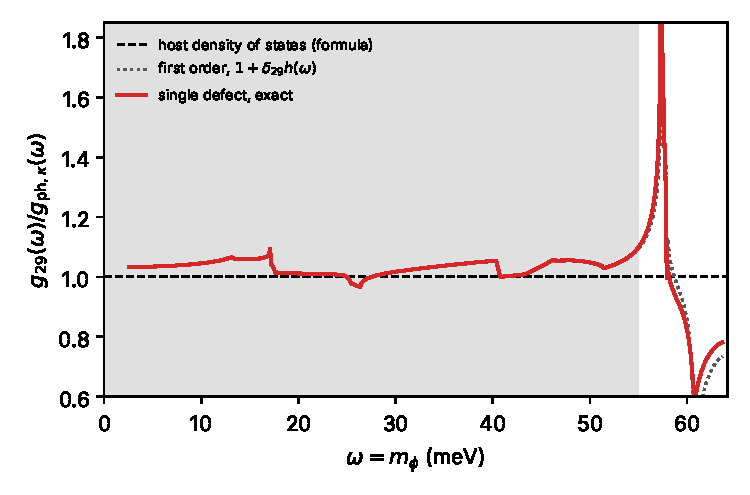
\includegraphics[width=\linewidth]{figures/ch11/limit11_6a.pdf}
\captionof{figure}{Rate of \cref{eq:11.6-alp} for natural silicon, where the spin sits on $^{29}$Si, with the exact local density of states of one $^{29}$Si atom from \cref{eq:11.6-lifshitz} (red), divided by the same rate with the host density of states (dashed, the formula), against the axion mass. The ratio $g_{29}/g_{\mathrm{ph},\kappa}$ does not depend on the couplings. Dotted: the first order in the mass defect, $1 + \delta_{29}h_{\mathrm{iso}}(\omega)$ with $\delta_{29} = -0.0317$, \cref{eq:11.6-first}. PBE density of states of \cref{sec:5.2}, $T = 0$. Gray: within \SI{10}{\percent} of the formula, $m_\phi < \SI{55.0}{meV} = 0.865\,\omega_{\mathrm{max}}$.}\label{fig:11-limit-6a}
\par}
\smallskip
Near the top of the optical band the heavier isotope moves weight from the band edge to just below it, and the host density of states errs by up to a factor of 2.
\end{limitbox}

Below \SI{55}{meV} the heavier spin carrier changes the rate by $-3.5$ to $+\SI{10}{\percent}$, mostly by 1 to \SI{5}{\percent} upward, and the first order of \cref{eq:11.6-first} reproduces the exact ratio to \SI{0.5}{\percent}. At the sharp lower edge of the optical band the ratio rises to about 2, with a peak of 2.05 at \SI{57.3}{meV} in the PBE spectrum, and between 60 and \SI{63}{meV} it falls to 0.6, with a minimum of 0.59 near \SI{60.7}{meV}. The band integral is unchanged, since both densities of states are normalized to three, so the weight is moved and not lost. This is the correlation between the vertex and the mass: the vertex sits on an atom whose mass, and therefore whose vibrations, differ from the average. Bloch and collaborators assume that the isotopes leave the phonon spectrum unchanged, which holds for the crystal as a whole when one isotope dominates~\cite[footnote~5]{bloch2025broadband}. The local spectrum at a minority isotope still differs, and in silicon the host density of states is good to \SI{10}{\percent} over \SI{86}{\percent} of the band.

\Cref{eq:11.6-lifshitz} itself treats one defect in a perfect host. How far does it carry into a crystal that contains many?

\begin{limitbox}[Lifshitz mass-defect Green function][lim:11.6b]
One atom of mass $\bar M(1 - \delta^M)$ in a harmonic host: $\GF_i = \GF_{\mathrm{h}}/(1 + \delta^M\bar M\omega^2\GF_{\mathrm{h}})$ on its site~\cites{lifshitz1956some}{dawber1963vibrations}.
\par\smallskip
{\centering
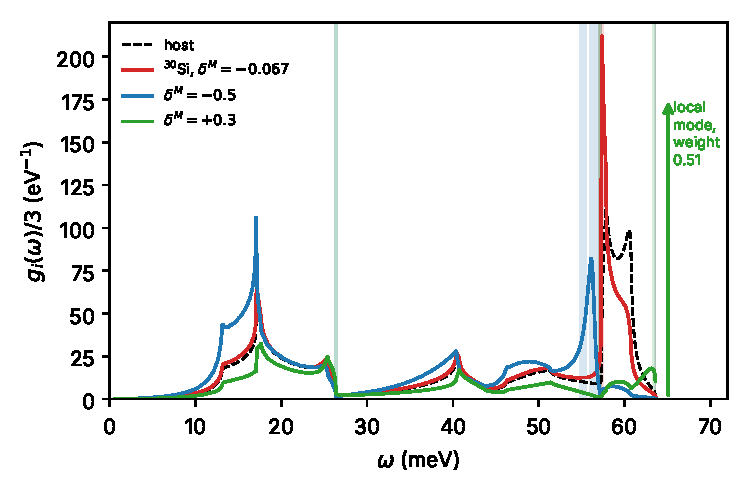
\includegraphics[width=\linewidth]{figures/ch11/limit11_6b.pdf}
\captionof{figure}{Local density of states per direction, $g_i(\omega)/3$, of one mass defect in silicon from \cref{eq:11.6-lifshitz}, with the PBE density of states of \cref{sec:5.2} (dashed, the host). Red: $^{30}$Si, $\delta^M = -0.067$. Blue: a heavy defect, $\delta^M = -0.5$. Green: a light defect, $\delta^M = +0.3$, which puts \SI{51}{\percent} of its weight into a local mode at \SI{65.1}{meV}, above the band (arrow). The integral of each curve, local mode included, is one. Shaded in the color of each curve: frequencies where the leading pair term exceeds \SI{10}{\percent}. The pair term is the effect of a second defect anywhere in the crystal on the first, for the natural isotope mixture around $^{30}$Si and for a concentration of \SI{1}{\percent} of the strong defects; pair term to first order in the scattering of the second defect, from the host Green function.}\label{fig:11-limit-6b}
\par}
\smallskip
The single-defect form fails where defects interact: within a meV of the sharp edges of the host density of states in natural silicon, and over windows of a few meV around them for defects of tens of percent in mass at concentrations of a percent.
\end{limitbox}

The pair term in the caption needs no new calculation. A second defect $j$ at site $\vect{r}$ changes the host function on site $I$ to $\GF_{\mathrm{h}} + \GF_{I\vect{r}}t_j\GF_{\vect{r}I}$, with $t_j = -\delta^M_j\bar M\omega^2/(1 + \delta^M_j\bar M\omega^2\GF_{\mathrm{h}})$ its scattering strength, and the sum over all $\vect{r} \neq I$ of $\GF_{I\vect{r}}\GF_{\vect{r}I}$ is $(\GF^2)_{II} - \GF_{\mathrm{h}}^2 = \partial\GF_{\mathrm{h}}/\partial(\bar M\omega^2) - \GF_{\mathrm{h}}^2$, since $\GF$ is the inverse of $\Phi - \bar M\omega^2$. For the natural mixture referenced to $\bar M$ the first order in the second defect cancels, $\sum_jx_j\delta^M_j = 0$, and what remains is of order $g_{\mathrm{md}} = \sum_jx_j(\delta^M_j)^2 = 2.0\times10^{-4}$, the mass variance of \cref{app:E.12}. It is the self-energy behind the isotope scattering of phonons: its imaginary part gives the width $\frac{\pi}{2}g_{\mathrm{md}}\,\omega^2g_{\mathrm{ph},\kappa}(\omega)/3$, which at low frequency is the Rayleigh rate of \cref{eq:E.12-iso}, and at \SI{50}{meV} is $2.5\times10^{-4}$ of $\omega$. For $^{30}$Si in natural silicon the pair term stays below \SI{2.2}{\percent} up to \SI{55}{meV} and passes \SI{10}{\percent} only within a meV of the sharp edge of the optical band at \SI{57}{meV}. In silicon the isotopes can be treated one at a time.

\subsection{Absorption of a baryon-minus-lepton vector}\label{sec:11.6-bl}

A vector boson can couple to baryon number minus lepton number, $B - L$, with strength $g_{B-L}$, the same for protons and neutrons, $+g_{B-L}$, and for electrons, $-g_{B-L}$ (\cref{sec:1.4}). A neutral atom of isotope $i$, with $A_i$ nucleons and $Z$ electrons, carries the charge $A_i - Z = N_i$, its neutron number. Light enough, the vector can be the dark matter, and it is then absorbed like a dark photon. At rest it couples to the spatial current of its charges (\cref{sec:8.1-absorption}),
\begin{equation*}
  g_{B-L}\Bigl[\sum_\kappa A_\kappa\vect{j}_\kappa - \vect{j}_e\Bigr] = g_{B-L}\sum_\kappa N_\kappa\vect{j}_\kappa + g_{B-L}\Bigl[\sum_\kappa Z_\kappa\vect{j}_\kappa - \vect{j}_e\Bigr] .
\end{equation*}
The bracket $\sum_\kappa Z_\kappa\vect{j}_\kappa - \vect{j}_e$ is the electric current in units of $e$, and that part of the coupling is a dark photon with $\zeta = g_{B-L}/e$, and its rate is the dark-photon rate with in-medium mixing, $\zeta^2\sigma_1/|\varepsilon|^2$ (\cref{sec:10.7}):
\begin{equation}
  \varGamma_{\mathrm{EM}} = \Bigl(\frac{g_{B-L}}{e}\Bigr)^2\omega\,\Imag\Bigl[-\frac{1}{\varepsilon(\omega)}\Bigr] ,
  \label{eq:11.6-GEM}
\end{equation}
at $\omega = m_\phi$, with $\sigma_1 = \omega\varepsilon_2$. In silicon this part creates no single phonon. Its one-phonon vertex is the Born charge, and the Born charges of silicon vanish (\cref{sec:5.5}). Below the electronic gap it is absorbed only by pairs of phonons, through the dipole that a displacement induces on top of another, which is the weak lattice absorption of silicon in the far infrared.

The neutron-number current $g_{B-L}\sum_\kappa N_\kappa\vect{j}_\kappa$ couples each nucleus to its neutron number. In a crystal of one isotope the vertex is $\ii\omega g_{B-L}N_\kappa\hat{\vect{\epsilon}}$, with $\hat{\vect{\epsilon}}$ the polarization of the vector. It is proportional to $M_\kappa$ on both sites of silicon, and the coupling-to-mass cancellation removes it: a monatomic crystal of one isotope does not absorb a $B - L$ vector into one phonon at all. Natural silicon does, because the neutron number per unit mass,
\begin{equation*}
  \mathfrak{b}_i = \frac{N_i}{M_i} ,
\end{equation*}
is $0.5004$, $0.5177$ and \SI{0.5338}{u^{-1}} for the three isotopes. The mass-proportional part of the vertex is set by the mass-weighted mean $\bar{\mathfrak{b}} = \sum_ix_iN_i/\sum_ix_iM_i = \SI{0.50235}{u^{-1}}$, with $x_i$ the abundances, and the remainder $\delta\vect{v}_I = \ii\omega g_{B-L}M_i(\mathfrak{b}_i - \bar{\mathfrak{b}})\hat{\vect{\epsilon}}$ has zero mean and is independent from site to site. Its direction is fixed, but on a cubic site every direction gives the same projection of the local density of states. \Cref{eq:11.6-random} with the vertex in $S_{OO}$ and \cref{eq:8.2-abs} give, per absorbed quantum at $T = 0$ and with $\Omega_{\mathrm{at}}$ the volume per atom,
\begin{keyresult}[Isotope-disorder absorption of a $B - L$ vector]
\begin{equation}
  \begin{aligned}
  \varGamma_{\mathrm{iso}}(\omega) &= \frac{\pi g_{B-L}^2}{2\Omega_{\mathrm{at}}}\sum_ix_iM_i(\mathfrak{b}_i - \bar{\mathfrak{b}})^2\,\frac{g_i(\omega)}{3} \\
  &= \frac{\pi g_{B-L}^2\bar M\sigma_{\mathfrak{b}}^2}{2\Omega_{\mathrm{at}}}\,\frac{g_{\mathrm{ph},\kappa}(\omega)}{3}\Bigl[1 + \langle\delta^M\rangle_{\mathfrak{b}}\,h_{\mathrm{iso}}(\omega) + O(g_{\mathrm{md}})\Bigr] ,
  \end{aligned}
  \label{eq:11.6-Giso}
\end{equation}
at $\omega = m_\phi$ inside the one-phonon band and zero above it, with $\sigma_{\mathfrak{b}}^2 = \sum_ix_i(M_i/\bar M)(\mathfrak{b}_i - \bar{\mathfrak{b}})^2$ the mass-weighted variance of $\mathfrak{b}$ and $\langle\delta^M\rangle_{\mathfrak{b}}$ the mass defect averaged with the weights $x_iM_i(\mathfrak{b}_i - \bar{\mathfrak{b}})^2$. In natural silicon $\sigma_{\mathfrak{b}}^2/\bar{\mathfrak{b}}^2 = 1.88\times10^{-4}$ and $\langle\delta^M\rangle_{\mathfrak{b}} = -0.054$.
\end{keyresult}
\noindent The two parts of the coupling reach different final states, one phonon or two, and they add without interference. The isotope phonons do not mix with the photon either, since the Born charge of every silicon atom vanishes whatever its mass. The vertex of an isotope sits on the atom whose mass differs. The isotope-resolved form of \cref{eq:11.6-Giso} takes this into account through the local density of states of each isotope, \cref{eq:11.6-lifshitz}, and the terms between different sites, which vanish to first order in the mass defects, are the pair terms of \cref{lim:11.6b}. A vector coupled to baryon number alone would see almost nothing. Its charge per mass, $A_i/M_i$, differs between the isotopes only through their binding energies, and the variance is $9\times10^{-11}$ of the squared mean, two million times below that of $B - L$.

How large is the isotope channel against the electromagnetic one? The answer depends on the temperature, through the two-phonon absorption. Consider a pair process in which the field is absorbed and two phonons of energies $\omega_1$ and $\omega_2$ are created, $\omega = \omega_1 + \omega_2$. Its rate is proportional to $(1 + n_1)(1 + n_2)$ and that of the reverse process, stimulated emission, to $n_1n_2$, with the Bose occupations $n_{1,2}$, so the net absorption carries $1 + n_1 + n_2 \ge 1$. In a difference process a phonon $\omega_2$ is absorbed and a phonon $\omega_1 = \omega + \omega_2$ created, with the net weight $n_2(1 + n_1) - n_1(1 + n_2) = n_2 - n_1 \ge 0$, which vanishes at $T = 0$. Suppose the second-order dipole moments and the phonon frequencies do not depend on temperature. Then every term of the absorption coefficient falls as the crystal cools, and
\begin{equation}
  \alpha(\omega; T \to 0) \le \alpha(\omega; \SI{293}{K}) .
  \label{eq:11.6-Tbound}
\end{equation}
The frequencies do shift, by about \SI{1}{\percent} between room temperature and zero, and the lines narrow, so the inequality holds for the absorption integrated over a window wider than the shift and the room-temperature width; where the room-temperature spectrum is flat over that window, it holds point by point. Below the top of the one-phonon band the far-infrared absorption of silicon at room temperature is dominated by difference processes~\cite{ikezawa1981far}, which freeze out completely, so the bound is far from saturated at millikelvin temperatures.

\begin{workedexample}{The isotope channel against the electromagnetic one at \SI{50}{meV}}\label{we:11-iso}
Take natural silicon and $m_\phi = \SI{50}{meV}$, inside the one-phonon band. With $\bar{\mathfrak{b}} = \SI{0.50235}{u^{-1}}$ and $\sigma_{\mathfrak{b}}^2 = 1.879\times10^{-4}\,\bar{\mathfrak{b}}^2 = \SI{4.742e-5}{u^{-2}}$, the product $\bar M\sigma_{\mathfrak{b}}^2 = \SI{1.332e-3}{u^{-1}}$ is \SI{1.430e-12}{eV^{-1}} with $\SI{1}{u} = \SI{931.494}{MeV}$. The PBE density of states of \cref{sec:5.2} gives $g_{\mathrm{ph},\kappa}/3 = \SI{15.9}{eV^{-1}}$ at \SI{50}{meV}, and the volume per atom is $\Omega_{\mathrm{at}} = a^3/8 = \SI{20.02}{\angstrom^3} = \SI{2.606e-9}{eV^{-3}}$. \Cref{eq:11.6-Giso} with the host density of states gives
\begin{equation*}
  \frac{\varGamma_{\mathrm{iso}}}{g_{B-L}^2} = \frac{\pi\times\SI{1.430e-12}{eV^{-1}}\times\SI{15.9}{eV^{-1}}}{2\times\SI{2.606e-9}{eV^{-3}}} = \SI{1.37e-2}{eV} .
\end{equation*}
The correction for the heavier carriers of the vertex is $\langle\delta^M\rangle_{\mathfrak{b}}h_{\mathrm{iso}} = (-0.054)(-1.55) = +\SI{8.3}{\percent}$ to first order, with $h_{\mathrm{iso}}(\SI{50}{meV}) = -1.55$ from the same density of states; the exact single-defect densities give $+\SI{8.0}{\percent}$, and $\varGamma_{\mathrm{iso}}/g_{B-L}^2 = \SI{1.48e-2}{eV}$.

For the electromagnetic part we need $\Imag(-1/\varepsilon)$ at \SI{50}{meV} (\SI{403}{cm^{-1}}). The measured absorption coefficient of silicon at \SI{293}{K} is $\alpha = \SI{0.55}{cm^{-1}}$ there~\cite{ikezawa1981far}; we read it off a published figure~\cite[Fig.~3]{deinzer2004two}, and the reading is uncertain by about \SI{10}{\percent}. With $\varepsilon_2 = \alpha n_r/\omega$, $n_r = 3.42$ and $\omega = \SI{2534}{cm^{-1}}$ as an inverse length ($2\pi$ times the wavenumber), $\varepsilon_2 = 7.43\times10^{-4}$, and with $\varepsilon_1 = 11.7$, $\Imag(-1/\varepsilon) = \varepsilon_2/(\varepsilon_1^2 + \varepsilon_2^2) = 5.42\times10^{-6}$. \Cref{eq:11.6-GEM} with $e^2 = 4\pi\alpha = 0.0917$ gives $\varGamma_{\mathrm{EM}}/g_{B-L}^2 = \SI{0.050}{eV}\times5.42\times10^{-6}/0.0917 = \SI{2.96e-6}{eV}$. By \cref{eq:11.6-Tbound} this is an upper bound at millikelvin temperatures, and
\begin{equation*}
  \frac{\varGamma_{\mathrm{iso}}}{\varGamma_{\mathrm{EM}}} \ge \frac{\SI{1.48e-2}{eV}}{\SI{2.96e-6}{eV}} = 5.0\times10^3 \qquad (\SI{50}{meV},\ T \to 0).
\end{equation*}
At \SI{50}{meV}, in a valley of the density of states between the longitudinal acoustic and optical features, the PBE spectrum, softer by about \SI{1}{\percent} than the room-temperature neutron data of \cref{sec:5.2}, shifts $g_{\mathrm{ph},\kappa}$ by a comparable amount. Neither this nor the reading of $\alpha$ changes the conclusion: in a cold silicon crystal a $B - L$ vector of \SI{50}{meV} is absorbed by the isotopes thousands of times more often than by the electromagnetic channel.
\end{workedexample}

\Cref{fig:11-iso} shows the two channels across the band. The isotope channel follows the density of states, from the acoustic peaks near \SI{17}{meV} to the optical peak near \SI{58}{meV}, and vanishes at the top of the band. Against the room-temperature electromagnetic bound it wins by factors from $2\times10^2$, at the top of the band where the density of states falls to zero, to $1.4\times10^4$. Above the band only the electromagnetic part remains, and at the two-phonon peak near \SI{76}{meV} it is 17 times stronger than at \SI{50}{meV}. The size of the isotope channel is set by the isotopic variance: a crystal enriched in $^{28}$Si suppresses it in proportion to the depletion of the minority isotopes, while the electromagnetic part is unchanged, which makes enrichment a control of the signal.

\begin{figure}[tbp]
  \centering
  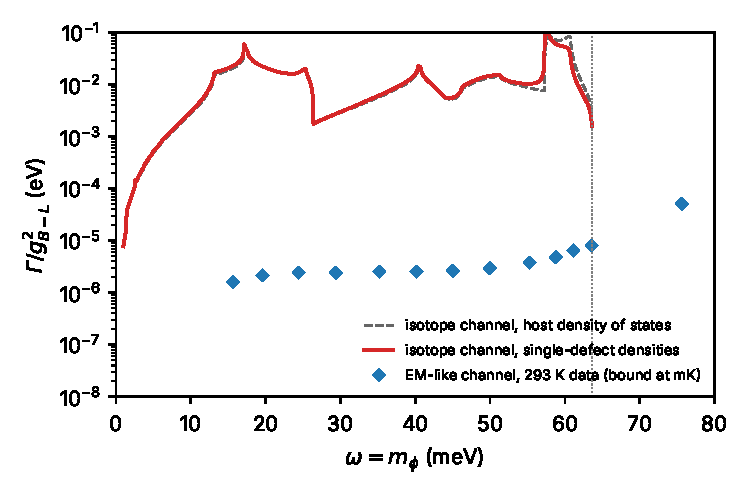
\includegraphics[width=0.8\linewidth]{figures/ch11/fig11_6.pdf}
  \caption{Absorption rate per quantum of a $B - L$ vector in natural silicon, over the squared coupling, against its mass. Red: the isotope-disorder channel of \cref{eq:11.6-Giso} with the exact single-defect densities of states of the three isotopes, \cref{eq:11.6-lifshitz}; dashed: the same with the host density of states for all. PBE phonons of \cref{sec:5.2}, $T = 0$; the dotted line marks the top of the PBE band, \SI{63.7}{meV} (the measured band top is \SI{64.1}{meV}). Blue diamonds: the electromagnetic channel \cref{eq:11.6-GEM}, from the measured absorption coefficient at \SI{293}{K} of Ikezawa and Ishigame~\cite{ikezawa1981far}, read from Fig.~3 of Deinzer and Strauch~\cite{deinzer2004two} with an uncertainty of about \SI{0.05}{cm^{-1}} plus \SI{10}{\percent}, converted with $n_r = 3.42$ and $\varepsilon_1 = 11.7$. At millikelvin temperatures the diamonds are upper bounds, \cref{eq:11.6-Tbound}. The diamond at \SI{76}{meV} is the two-phonon peak, above the one-phonon band.}
  \label{fig:11-iso}
\end{figure}

The inputs of these rates come from one harmonic calculation of the pure crystal. Its density of states and \cref{eq:11.6-lifshitz} give the local density of states of every isotope, and the force constants are those of \cref{sec:5.2} and \cref{app:E.4}. The exact rate of a disordered crystal includes every isotope and the pair terms. It comes from diagonalizing the Hessian of a supercell of a few thousand atoms with the isotopes drawn at random, and \cref{app:E.17} specifies that calculation; the single-defect correction of \cref{eq:11.6-Giso} is its check. The spin expectation values $\langle S_p\rangle$ and $\langle S_n\rangle$ of each odd isotope, which set $g_{ai}$ and $c_4^{(i)}$, come from nuclear shell-model calculations, and \cref{app:E.27} specifies them with their spread.

One input is missing. The electromagnetic channel of \cref{eq:11.6-GEM} needs $\varepsilon(\omega)$ of silicon inside the one-phonon band at the temperature of the detector, and we know of no measurement of the two-phonon absorption of silicon below \SI{65}{meV} at low temperature. The room-temperature data give only the bound \cref{eq:11.6-Tbound}, dominated by difference processes that are absent in a cold crystal. The zero-temperature absorption requires the second-order dipole moments, the derivatives of the Born charges with respect to the displacements, which a first-principles calculation can supply (\cref{app:E.17}); until it or a cold measurement exists, the margin of $5\times10^3$ at \SI{50}{meV} is a lower limit.

\section{Anisotropy and daily modulation}\label{sec:11.7}

At $45^\circ$N the dark-matter wind arrives from almost straight overhead when Cygnus crosses the meridian, and from close to the horizon twelve sidereal hours later (\cref{fig:1-daily}). A crystal fixed to the laboratory floor is therefore probed along different crystal directions in the course of each sidereal day. An isotropic target such as a liquid has the same rate in every orientation; a crystal responds differently along different crystal axes, so its rate follows the sidereal day. The size of the effect differs widely between crystals: below \SI{1}{\percent} in silicon, for electron recoils and for phonons alike, and \SI{6}{\percent} for multiphonon events in sapphire above a threshold of \SI{300}{meV}. Two factors set it, the angular structure of the crystal response and the sharpness with which the halo singles out one direction of $\vect{q}$, and the two can be computed separately, for the electronic responses of \cref{chap:10} and the nuclear responses of this chapter alike.

\subsection{Rate at fixed orientation}

Take a coupling through one density, the electron density of \cref{sec:10.1} or the nuclear operator of \cref{sec:11.1}, with a potential $\tilde V(q)$ that depends only on $|\vect{q}|$. The rate per unit target mass is \cref{eq:8.2-spectrum} with one row, $\mathfrak{D} = |\tilde V(q)|^2$, and the direction of $\vect{q}$ enters both the structure factor $S(\vect{q},\omega)$ and the velocity kernel $\int\dd^3v\,f_\chi(\vect{v})\,\delta(\omega - \omega_{\vect{q}})$. For elastic scattering, $\omega_{\vect{q}} = \vect{q}\cdot\vect{v} - q^2/2\mchi$ (\cref{eq:A.4-omegaq}), and the delta function becomes $q^{-1}\delta(\hat{\vect{q}}\cdot\vect{v} - \vmin)$ with $\vmin = \omega/q + q/2\mchi$ (\cref{eq:1.3-vmin}). The laboratory distribution is the galactic one shifted by the Earth's velocity, $f_\chi(\vect{v}) = f_{\mathrm{gal}}(\vect{v} + \vect{v}_{\mathrm{E}})$ (\cref{eq:1.2-flab}). Substituting $\vect{u} = \vect{v} + \vect{v}_{\mathrm{E}}$ turns the velocity integral into
\begin{equation*}
  \int\dd^3v\,f_\chi(\vect{v})\,\delta(\omega - \omega_{\vect{q}}) = \frac1q\int\dd^3u\,f_{\mathrm{gal}}(\vect{u})\,\delta\bigl(\hat{\vect{q}}\cdot\vect{u} - \vmin - v_{\mathrm{E}}\,\hat{\vect{q}}\cdot\hat{\vect{v}}_{\mathrm{E}}\bigr) = \frac1q\,\hat f_{\mathrm{gal}}\bigl(\vmin + v_{\mathrm{E}}x\bigr) ,
\end{equation*}
with $x = \hat{\vect{q}}\cdot\hat{\vect{v}}_{\mathrm{E}}$ the cosine of the angle between the momentum transfer and the Earth's velocity. The function $\hat f_{\mathrm{gal}}(s)$ is the integral of the isotropic galactic distribution over the plane $\hat{\vect{q}}\cdot\vect{u} = s$, the Radon transform of $f_{\mathrm{gal}}$. For the truncated Maxwellian of \cref{eq:1.2-fgal}, the two Gaussian integrals across the plane run over the disc $u_\perp^2 < v_{\mathrm{esc}}^2 - s^2$, and
\begin{equation*}
  \hat f_{\mathrm{gal}}(s) = \frac{\pi v_0^2}{N_{\mathrm{esc}}}\Bigl[\ee^{-s^2/v_0^2} - \ee^{-v_{\mathrm{esc}}^2/v_0^2}\Bigr]\,\Theta\bigl(v_{\mathrm{esc}} - |s|\bigr) ,
\end{equation*}
with $N_{\mathrm{esc}}$ of \cref{eq:1.2-nesc}. The halo enters only through this function of one variable, and the crystal only through $S(\vect{q},\omega)$ at fixed $|\vect{q}|$, a function on the sphere of directions.

Both factors are now expanded on the sphere. The halo factor is a function of $x$ alone and has a Legendre series, $\hat f_{\mathrm{gal}}(\vmin + v_{\mathrm{E}}x) = \sum_\ell\tfrac12(2\ell + 1)\,\mathcal{H}_\ell\,P_\ell(x)$, with coefficients
\begin{equation}
  \mathcal{H}_\ell(\vmin) = \int_{-1}^{1}\dd x\;P_\ell(x)\,\hat f_{\mathrm{gal}}\bigl(\vmin + v_{\mathrm{E}}x\bigr) ,
  \label{eq:11.7-ups}
\end{equation}
the multipoles of the halo. The crystal factor is expanded in real spherical harmonics $Y_{\ell m}$, the real and imaginary parts of those of \cref{app:C.3}, taken in crystal axes, with components $S_{\ell m}(|\vect{q}|,\omega) = \int\dd^2\hat{\vect{q}}\,Y_{\ell m}(\hat{\vect{q}})\,S(\vect{q},\omega)$. The addition theorem \cref{eq:C.3-addition} holds for the real harmonics too. It gives $\int\dd^2\hat{\vect{q}}\,P_\ell(\hat{\vect{q}}\cdot\hat{\vect{v}}_{\mathrm{E}})\,Y_{\ell'm}(\hat{\vect{q}}) = [4\pi/(2\ell + 1)]\,\delta_{\ell\ell'}\,Y_{\ell m}(\hat{\vect{v}}_{\mathrm{E}})$, and the angular integral pairs each multipole of the response with the halo multipole of the same order:
\begin{keyresult}[Rate of a crystal at fixed orientation]
\begin{equation}
  \frac{\dd\mathcal{R}}{\dd\omega}(t) = \frac{\rho_\chi}{\mchi\,\rho_T}\int\frac{q\,\dd q}{4\pi^2}\,|\tilde V(q)|^2\sum_{\ell m}\mathcal{H}_\ell\bigl(\vmin(q,\omega)\bigr)\,S_{\ell m}(q,\omega)\,Y_{\ell m}\bigl(\hat{\vect{v}}_{\mathrm{E}}(t)\bigr) ,
  \label{eq:11.7-rate}
\end{equation}
with $\hat{\vect{v}}_{\mathrm{E}}(t)$ the direction of the Earth's velocity in crystal axes, which turns with the sidereal day. For a cubic crystal the sum over $m$ at each order is one cubic harmonic $Y^{\mathrm{c}}_\ell$ of \cref{eq:C.3-cubic}, $\sum_mS_{\ell m}Y_{\ell m}(\hat{\vect{v}}_{\mathrm{E}}) = S_\ell\,Y^{\mathrm{c}}_\ell(\hat{\vect{v}}_{\mathrm{E}})$ with $S_\ell(|\vect{q}|,\omega) = \int\dd^2\hat{\vect{q}}\,Y^{\mathrm{c}}_\ell(\hat{\vect{q}})\,S(\vect{q},\omega)$, for $\ell \le 10$.
\end{keyresult}
\noindent The monopole term reproduces the isotropic rate. Since $\int_{-1}^1\dd x\,\hat f_{\mathrm{gal}}(\vmin + v_{\mathrm{E}}x)/2q$ is the average of the velocity integral over the directions of $\vect{q}$, which \cref{eq:A.8-eta} identified with $\eta/2q$, the zeroth halo multipole is the mean inverse speed, $\mathcal{H}_0(\vmin) = \eta(\vmin)$. With $S_{00}Y_{00} = \bar S$, the term $\ell = 0$ of \cref{eq:11.7-rate} is the isotropic rate of \cref{eq:A.8-eta}. The other terms carry all of the time dependence, through $Y_{\ell m}(\hat{\vect{v}}_{\mathrm{E}}(t))$, and each is weighted by the product of a property of the crystal, $S_{\ell m}$, and a property of the halo, $\mathcal{H}_\ell$. The same separation underlies the harmonic method of Al-Adulrazzaq and collaborators~\cite[Eqs.~(6), (10), (17)]{aladulrazzaq2026anisotropic}. Stratman and Lin integrate the same rate directly over the directions of $\vect{q}$~\cite[Eqs.~(28), (29), (31)]{stratman2025daily}. For a coupling with several rows, $|\tilde V|^2S$ becomes the contraction of \cref{eq:8.2-spectrum}; as long as $\mathfrak{D}_{ab}$ depends on $|\vect{q}|$ alone, each $S_{ab}$ is expanded in the same way. A coupling that depends on the dark-matter velocity puts powers of $\vect{v}$ under the velocity integral, and its halo factor is then no longer a function of $x$ alone.

How quickly the halo multipoles fall with $\ell$ decides how much of a crystal's anisotropy reaches the rate. With the standard halo of \cref{sec:1.2}, the ratio $\mathcal{H}_2/\mathcal{H}_0$ is 0.13, 0.37, 0.51 and 0.70 at $\vmin = 300$, 500, 600 and \SI{700}{km.s^{-1}}, while $\mathcal{H}_4/\mathcal{H}_0$ is only $-0.016$, $0.017$, $0.069$ and $0.27$. The reason is the shape of the halo factor. As a function of $x$ it is a Gaussian of width $v_0/v_{\mathrm{E}} = 0.95$, centered at $x = -\vmin/v_{\mathrm{E}}$: the momentum transfer prefers to point along the wind, against $\vect{v}_{\mathrm{E}}$, but only loosely, and a broad function has small high multipoles. Near the kinematic edge, $\vmin \to v_{\mathrm{esc}} + v_{\mathrm{E}}$, only a small cap of directions around $-\hat{\vect{v}}_{\mathrm{E}}$ is allowed, and every multipole approaches $\mathcal{H}_0$ in magnitude. At small $\vmin$ the preference reverses: a particle that needs only a small velocity component along $\vect{q}$ is best served by a $\vect{q}$ nearly perpendicular to its velocity, and $\mathcal{H}_2/\mathcal{H}_0 = -0.13$ at $\vmin = 0$. The quadrupole changes sign at $\vmin = \SI{196}{km.s^{-1}}$ and the hexadecapole at 138 and \SI{435}{km.s^{-1}}, so the phase of a modulation can flip with the mass or the energy deposited, as the annual modulation does at \SI{211}{km.s^{-1}} (\cref{sec:1.2}). The halo therefore filters the anisotropy of a crystal: the quadrupole passes at the level of tens of percent, the hexadecapole at a few percent, and the higher orders only for the fastest particles.

We measure the result by the daily-modulation amplitude
\begin{equation}
  A_{\mathrm{day}} = \frac{\mathcal{R}_{\mathrm{max}} - \mathcal{R}_{\mathrm{min}}}{\mathcal{R}_{\mathrm{max}} + \mathcal{R}_{\mathrm{min}}} ,
  \label{eq:11.7-Aday}
\end{equation}
the half-range of the rate over one sidereal day divided by its mean, for a rate integrated above a threshold. It depends on the crystal, on its mounting and on the latitude, which together fix the path of $\hat{\vect{v}}_{\mathrm{E}}(t)$ in crystal axes (\cref{eq:1.2-local}), and on the dark-matter mass and the threshold, which fix the values of $\vmin$ the rate samples.

\subsection{Selection rules}

The first restriction is evenness. With inversion symmetry, or with time-reversal symmetry, $S(\vect{q},\omega) = S(-\vect{q},\omega)$ (\cref{app:A.4}), and every component with odd $\ell$ vanishes. This holds in silicon, germanium and GaAs, with or without spin--orbit coupling, at every $|\vect{q}|$, every $\omega$ and every temperature, and for the loss function as well as for $S$. The odd halo multipoles are large, $\mathcal{H}_1/\mathcal{H}_0 = -0.54$ at \SI{300}{km.s^{-1}}, but no even response can use them.

A response with odd parts needs both symmetries broken, as in a magnetically ordered crystal without a center of inversion. For a density its odd part is then small at small momentum transfer. For $f \ne i$ the matrix element starts as $\langle f|n_e(\vect{q})|i\rangle = \ii\vect{q}\cdot\vect{d}_{fi} - \tfrac12q_\alpha q_\beta Q^{\alpha\beta}_{fi} + O(q^3)$, with $\vect{d}_{fi}$ and $Q^{\alpha\beta}_{fi}$ the matrix elements of $\sum_j\vect{r}_j$ and $\sum_jr^\alpha_jr^\beta_j$; the term of order zero vanishes by orthogonality. The difference between $\vect{q}$ and $-\vect{q}$ is the interference of the two leading terms,
\begin{equation*}
  |\langle f|n_e(\vect{q})|i\rangle|^2 - |\langle f|n_e(-\vect{q})|i\rangle|^2 = 2\,\Imag\bigl[(\vect{q}\cdot\vect{d}_{fi})\,q_\alpha q_\beta Q^{\alpha\beta*}_{fi}\bigr] + O(q^5) ,
\end{equation*}
which is of third order in $q$. Inversion forbids it, because $\vect{d}_{fi}$ connects states of opposite parity and $Q_{fi}$ states of the same parity; time reversal forbids it, because it makes both matrix elements real in a suitable basis. Where it survives, it multiplies the odd halo multipoles, and the rate acquires a part that is odd in the direction of the wind: opposite wind directions in crystal axes give it opposite signs. Such nonreciprocal targets are treated in \cref{sec:14.5}. A chiral crystal that keeps time reversal has an even $S$, and its two enantiomers modulate identically.

The second restriction is the point group. A function of direction invariant under the cubic group has no component with $\ell = 2$ (\cref{app:C.3}), so in silicon, germanium and GaAs the anisotropy of every response, electronic or nuclear, starts at $\ell = 4$ with $Y^{\mathrm{c}}_4$, followed by $Y^{\mathrm{c}}_6$ and $Y^{\mathrm{c}}_8$. A uniaxial crystal, such as trigonal sapphire or a hexagonal polytype of SiC, has one invariant direction, the $c$ axis $\hat{\vect{c}}$, and allows $\ell = 2$ with $m = 0$ about it. To this order the rate is $\mathcal{R}_0 + \mathcal{R}_2P_2(\hat{\vect{c}}\cdot\hat{\vect{v}}_{\mathrm{E}})$, the constant plus a constant times $\cos^2\theta_{\mathrm{lab}}$ that \cref{sec:1.2} wrote down by symmetry alone, and \cref{eq:11.7-rate} now supplies the two constants. At $\ell = 4$ a trigonal crystal adds terms with $|m| = 3$, and a hexagonal one first breaks the symmetry about $\hat{\vect{c}}$ at $\ell = 6$. Combined with the halo filter, the counting already explains the main pattern: for the same anisotropy of the response, a uniaxial crystal modulates through $\mathcal{H}_2$, a cubic one through $\mathcal{H}_4$, roughly ten times less except near the kinematic edge.

\subsection{Electronic anisotropy}

How anisotropic is the loss function of silicon? The covalent bonds point along the four $\langle111\rangle$ directions, the conduction-band minima lie along $\langle100\rangle$, and an electron--hole pair of a few eV made with a momentum transfer of a few keV feels both. \Cref{fig:11-aniso}(a) shows the ratio $L_4/L_0$ of the cubic-harmonic components of the loss function, in the empirical pseudopotential model of \cref{sec:3.3} that \cref{lim:10.1a} used, with the random-phase head of the dielectric matrix and no local fields. Each component is fitted to the loss function computed along ten directions of the irreducible wedge of the cube. The $k$ grid has the full cubic symmetry, so the components with $\ell = 2$ and odd $\ell$ vanish identically and cannot leak in as artifacts; refining it from $12^3$ to $16^3$ points changes $L_4/L_0$ by at most 0.01. At $q = q_0 = \SI{3.73}{keV}$ the ratio is 0.18 at \SI{3}{eV}, 0.05 at \SI{5}{eV} and below 0.01 above \SI{8}{eV}. The hexadecapole is not dominant: $L_6/L_0$ is of the same size, and near the gap the components beyond $\ell = 8$ carry an rms deviation of \SI{10}{\percent} of $\bar L$ or more, a sign of structure on small angular scales. Away from the gap the response is closer to that of a uniform gas, which has no preferred direction. GaAs, with the same lattice and a different basis, has components of the same size.

The halo multipoles now decide how much of this survives in the rate. \Cref{lim:11.7a} follows it at \SI{5}{eV} for a \SI{10}{MeV} particle. Wherever $\vmin$ is well below the kinematic edge, $\mathcal{H}_4/\mathcal{H}_0$ is a few percent and the anisotropic part of the rate at each $q$ stays below a few tenths of a percent, carried by the term $\ell = 4$ alone. Only near the edge, where the halo admits a narrow cone of directions, does the rate depend strongly on the direction of the wind, by tens of percent, and there the components $\ell \ge 6$ enter as well. Integrated over the spectrum of a \SI{2}{MeV} particle, the components combine into a daily modulation of about \SI{1}{\percent} (\cref{we:11-daily}).

These numbers are those of a model, and the model has two known gaps. The empirical pseudopotential reproduces the bands, not the wavefunctions at large momentum, and the calculation stops at $q = 2.8\,q_0$. Local fields add the crystal's own reciprocal vectors to the response at $q + \vect{G}$ and are known to change the direction-averaged rate by a factor of 1.3 to 1.5 at \SI{10}{MeV} (\cref{sec:10.2}); their effect on $L_4$ has not been computed. The cubic-harmonic components of the silicon loss function from a first-principles calculation with local fields, on a grid of directions fine enough for the structure near the gap, are therefore an open quantity. So, with them, is the electronic daily modulation of silicon beyond a model estimate. The calculation is specified in \cref{app:E.16}: the full-$\vect{q}$ loss function on Lebedev grids of increasing order, projected on $Y^{\mathrm{c}}_\ell$ for $\ell = 4$, 6 and 8, with the components $\ell = 1$, 2 and 3 as built-in tests that must vanish.

Evenness also settles a point in the literature. Al-Adulrazzaq and collaborators compute the electronic daily modulation of silicon and GaAs at \SI{10}{MeV} from the full loss function and find about one percent. They attribute the nearly sinusoidal shape of the signal at \SI{5}{eV}, with one period per sidereal day, to the dipole component of the loss function~\cite[Sect.~III\,B]{aladulrazzaq2026anisotropic}. The dipole component vanishes identically in both crystals, as do all odd components. A period of one sidereal day does not need $\ell = 1$: when the crystal axes are tilted with respect to the Earth's axis, $Y^{\mathrm{c}}_4(\hat{\vect{v}}_{\mathrm{E}}(t))$ contains every harmonic of the sidereal frequency up to the fourth, and which one dominates depends on the mounting. Their Migdal rate in the soft limit, in which the electronic and nuclear momenta separate, depends on the loss function only through its components with $\ell = 0$ and 2 at each $|\vect{k}|$~\cite[Eqs.~(37)--(41)]{aladulrazzaq2026anisotropic}. In a cubic crystal the component $\ell = 2$ vanishes at every $|\vect{k}|$, so the soft-limit Migdal rate of silicon, germanium and GaAs has no daily modulation at all. Their computed modulation of the Migdal rate is much smaller than that of the electron rate, as it must be, and any residue is numerical. Beyond the soft limit the Migdal response is the subject of \cref{chap:12}.

\subsection{Nuclear anisotropy}

The nuclear response carries its direction dependence in two places. In the incoherent approximation \cref{eq:11.3-inc}, each nucleus enters through its Debye--Waller exponent $2W_\kappa(\vect{q}) = \vect{q}\cdot B_\kappa\cdot\vect{q}$ (\cref{eq:5.6-W}) and through the spectrum $P^\kappa_1(\hat{\vect{q}},\omega)$, which is built from the density of states projected on $\hat{\vect{q}}$. Both are quadratic forms in $\hat{\vect{q}}$. The projected density of states is $\hat{\vect{q}}\cdot D_\kappa(\omega)\cdot\hat{\vect{q}}$, with the tensor
\begin{equation*}
  D^{\alpha\beta}_\kappa(\omega) = \frac1N\sum_{\vect{Q}\nu}\Real\bigl[e^\alpha_{\kappa\nu}(\vect{Q})\,e^{\beta}_{\kappa\nu}(\vect{Q})^*\bigr]\,\delta(\omega - \omega_{\vect{Q}\nu}) ,
\end{equation*}
whose trace is the atom-projected density of states $g_{\mathrm{ph},\kappa}(\omega)$ and whose integral against $\coth(\omega/2T)/(2M_\kappa\omega)$ is $B_\kappa$. Stratman and Lin write the incoherent response with this tensor and compute its daily modulation in sapphire and SiC~\cite[Eqs.~(18)--(24)]{stratman2025daily}. At a site of cubic symmetry every second-rank tensor is a multiple of the unit tensor (\cref{app:C.3}). Then $B_\kappa = \langle u_x^2\rangle\mathbb{1}$ and $D_\kappa = (g_{\mathrm{ph},\kappa}/3)\mathbb{1}$, and the direction of $\vect{q}$ drops out of \cref{eq:11.3-inc} term by term:
\begin{keyresult}[Isotropy of the incoherent response of cubic crystals]
If every nucleus sits at a site of cubic symmetry, the incoherent nuclear response \cref{eq:11.3-inc} is independent of the direction of $\vect{q}$ at every phonon order and every temperature. The direction dependence of the harmonic nuclear response of silicon, germanium, diamond and GaAs is entirely in its distinct part, the pair terms of \cref{eq:11.3-exact}.
\end{keyresult}
\noindent The temperature enters only through the Bose factors, which multiply each phonon by a scalar, so the statement holds at any $T$. The published tensors of Stratman and Lin show it to numerical precision: for silicon the three diagonal elements of $B_\kappa$ agree to $2\times10^{-4}$ and the off-diagonal ones are below \SI{e-7}{\angstrom^2}, and the two sites of GaAs agree to $8\times10^{-4}$. Their finding that the multiphonon rates of silicon and GaAs do not modulate~\cite[Sect.~IV]{stratman2025daily} is therefore exact within their approximation, not a numerical accident.

The anisotropy of the cubic nuclear response is entirely in the coherent terms, and \cref{sec:11.3} computed them. At long wavelength the one-phonon weight per direction is $\sum_\nu(\hat{\vect{q}}\cdot\hat{\vect{e}}_\nu)^2/c_\nu(\hat{\vect{q}})$ of \cref{eq:11.1-Sac}. With the measured elastic constants of \cref{sec:11.1} its component $\ell = 4$ is $S_4/S_0 = 0.028$, and $\ell = 6$ is below $10^{-3}$. The PBE force constants of \cref{sec:5.2} give $S_4/S_0 = 0.025$ for $q \le 0.3\,q_{\mathrm{BZ}}$, and the dispersion of the branches raises $|S_6/S_0|$ to 0.026 at $0.7\,q_{\mathrm{BZ}}$. Beyond the zone the one-phonon weight is strongly anisotropic. Near each reciprocal-lattice vector the acoustic phonons at $\vect{q} - \vect{G}$ are soft and their weight $1/\omega$ is large. The vectors $\vect{G}$ of a shell point in definite directions, and the weight is concentrated along them: just beyond the shell $|\vect{G}_{111}| = \SI{3.95}{keV} = 1.76\,q_{\mathrm{BZ}}$, at $q = 1.79\,q_{\mathrm{BZ}}$, $S_4/S_0 = -0.36$, and $S_6/S_0$ reaches $-0.49$ at $2.9\,q_{\mathrm{BZ}}$; beyond $5\,q_{\mathrm{BZ}}$, $|S_4/S_0|$ still reaches 0.2 and $|S_6/S_0|$ 0.4. The two-phonon weight, a sum over pairs of the square of a correlation, is less anisotropic, with $|S_4/S_0|$ and $|S_6/S_0|$ of about 0.1 at most. From three phonons on the incoherent part dominates, and the coherent corrections, and with them the anisotropy, are below \SI{3}{\percent} (\cref{sec:11.3}). These components come from the same force constants and the same pair correlations as the direction-averaged weights of \cref{sec:11.3}, and \cref{app:E.17} specifies their tabulation for silicon, germanium and GaAs, with the incoherent components $\ell \ge 4$ as a test that must vanish to numerical noise.

A cubic crystal therefore modulates through its nuclear response by less than \SI{1}{\percent}, and appreciably just at masses whose largest momentum transfer, $2\mchi v_{\mathrm{max}}$, ends close to a shell of reciprocal-lattice vectors, where the halo multipoles are large and one shell dominates. In silicon that happens near 1 and \SI{2}{MeV} (\cref{we:11-daily}). At other masses the shells inside the kinematic range contribute with alternating signs and largely cancel, and above a few MeV the incoherent part dominates the rate: the amplitude is \SI{0.04}{\percent} at 3 and \SI{4}{MeV} and $10^{-4}$ at 5 and \SI{10}{MeV}.

A crystal whose nuclei sit at sites of lower symmetry has an anisotropic incoherent response already. To first order in the anisotropy of $B_\kappa$, write $\vect{q}\cdot B_\kappa\cdot\vect{q} = q^2[\bar b_\kappa + \tfrac23\Delta b_\kappa P_2(\hat{\vect{c}}\cdot\hat{\vect{q}})]$ for a uniaxial site, with $\bar b_\kappa = \tfrac13\Tr B_\kappa$ and $\Delta b_\kappa = B^{cc}_\kappa - B^{aa}_\kappa$ the difference between the elements along and across the axis. The Poisson weight $p^{\mathrm{ph}}_n = \ee^{-2W_\kappa}(2W_\kappa)^n/n!$ of $n$ phonons (\cref{eq:5.6-poisson}) changes by $\delta(2W_\kappa)(n/2W_\kappa - 1)$ in its logarithm, so that
\begin{equation}
  \frac{\delta p^{\mathrm{ph}}_n}{p^{\mathrm{ph}}_n} = \bigl(n - 2\bar W_\kappa\bigr)\,\frac{2\Delta b_\kappa}{3\bar b_\kappa}\,P_2(\hat{\vect{c}}\cdot\hat{\vect{q}}) ,
  \label{eq:11.7-dw}
\end{equation}
with $2\bar W_\kappa = q^2\bar b_\kappa$. Orders below the mean phonon number lose weight along the axis of larger displacement and orders above it gain. A threshold well inside the multiphonon tail needs $n$ far above $2\bar W_\kappa$. The rate above it therefore inherits the anisotropy of $B_\kappa$ multiplied by the phonon number, while the projected spectrum $P^\kappa_1(\hat{\vect{q}},\omega)$ adds an anisotropy of its own whenever the threshold cuts through the phonon band. For sapphire the published tensors give, weighted with $A_\kappa^2$ over the four Al and six O sites of the cell, $B^{cc}/B^{aa} - 1 = +0.059$; for 2H-SiC only $+0.008$, because the larger displacement along the axis of the Si sites is partly offset by the C sites.

\begin{limitbox}[Daily modulation from the anisotropic response][lim:11.7a]
The rate of a crystal at fixed orientation pairs each multipole $S_{\ell m}$ of the response with the halo multipole $\mathcal{H}_\ell$ of the same order, $\dd\mathcal{R}/\dd\omega(t) = (\rho_\chi/\mchi\rho_T)\int q\,\dd q\,(4\pi^2)^{-1}|\tilde V|^2\sum_{\ell m}\mathcal{H}_\ell S_{\ell m}Y_{\ell m}(\hat{\vect{v}}_{\mathrm{E}}(t))$, \cref{eq:11.7-rate}, for the loss function~\cite[Eqs.~(10), (25)]{aladulrazzaq2026anisotropic} and for the incoherent nuclear response with direction-dependent Debye--Waller exponents and projected densities of states~\cite[Eqs.~(19), (24)]{stratman2025daily}. Its first anisotropic term is $\ell = 4$ in a cubic crystal and $\ell = 2$ in a uniaxial one.
\par\smallskip
{\centering
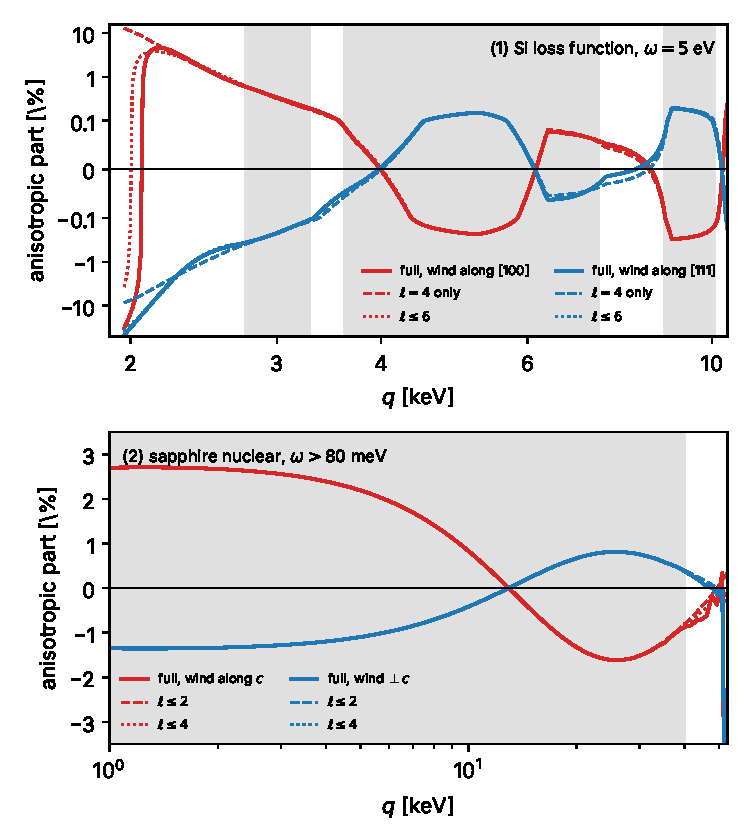
\includegraphics[width=\linewidth]{figures/ch11/limit11_7a.pdf}
\captionof{figure}{Anisotropic part of the rate at fixed momentum transfer for a wind along a fixed crystal axis, $\sum_{\ell \ge 1}\mathcal{H}_\ell\sum_mS_{\ell m}Y_{\ell m}(\hat{\vect{n}})/(\mathcal{H}_0S_{00}Y_{00})$ from \cref{eq:11.7-rate}, against $q$, for $\mchi = \SI{10}{MeV}$, a heavy mediator and the standard halo of \cref{sec:1.2}. (1) Silicon loss function at $\omega = \SI{5}{eV}$ in the empirical pseudopotential model (random-phase head, no local fields), wind along [100] (red) and [111] (blue), from the kinematic edge to the end of the model at $2.8\,q_0$; solid: all fitted components to $\ell = 8$; dashed: $\ell = 4$ alone, the formula; dotted: $\ell \le 6$, the leading correction (symmetric logarithmic axis, linear below \SI{0.1}{\percent}). (2) Sapphire, incoherent nuclear response with direction-dependent Debye--Waller exponents and projected densities of states from the site tensors of Stratman and Lin, integrated above \SI{80}{meV}, wind along the $c$ axis (red) and perpendicular to it (blue); solid: direct integral over the directions of $\vect{q}$; dashed: $\ell \le 2$, the formula; dotted: $\ell \le 4$. Gray bands: $q$ where the truncation at $\ell \le 4$ is within \SI{10}{\percent} of the full anisotropic part (or within $10^{-4}$ of the rate where that part is below $10^{-3}$): in panel (1) from \SI{2.7}{keV} up, except near 3.4, 8 and \SI{10}{keV}, where $\mathcal{H}_4$ or $L_4$ passes close to zero and $\ell = 6$ takes over; in panel (2) up to \SI{40}{keV}, against an edge at \SI{53}{keV}.}\label{fig:11-limit-7a}
\par}
\smallskip
Near the kinematic edge, where the halo admits only a narrow cone of directions, every multipole contributes, and a rate computed from the first anisotropic term alone misses the anisotropy there.
\end{limitbox}

\subsection{Daily-modulation amplitudes}

The time dependence comes from the path of $\hat{\vect{v}}_{\mathrm{E}}(t)$ in crystal axes. In equatorial axes the wind direction stays on a cone of half-angle $\theta_{\mathrm{E}} = 42.5^\circ$ around the Earth's rotation axis, and \cref{eq:1.2-local} gives its components along the local east, north and vertical. A crystal mounted with its axes along these three directions sees $\hat{\vect{v}}_{\mathrm{E}}(t)$ with exactly these components, and any other mounting is a fixed rotation of them. The amplitude of a term $\ell$ is then the range of $\sum_mS_{\ell m}Y_{\ell m}$ along the path. For a uniaxial crystal with its $c$ axis vertical at $45^\circ$N, the angle to the wind runs from $2.5^\circ$ to $87.5^\circ$, and $P_2$ sweeps from 0.997 to $-0.497$, nearly its full range. For a cubic crystal with [001] vertical at the same latitude, $Y^{\mathrm{c}}_4$ runs from $-0.39$ to $0.64$, close to its full range of $-0.43$ at [111] to $0.65$ at [100]. The rate oscillates mainly at twice the sidereal frequency, with a maximum when the wind arrives from overhead, along [001]. A cubic crystal mounted with [001] along the Earth's axis instead sees the wind circle at a fixed angle of $42.5^\circ$ from [001]. Then $Y^{\mathrm{c}}_4$ varies through its azimuthal part alone, $\cos4\varphi$, which gives four maxima per sidereal day and an amplitude six to ten times smaller.

\begin{figure}[tbp]
  \centering
  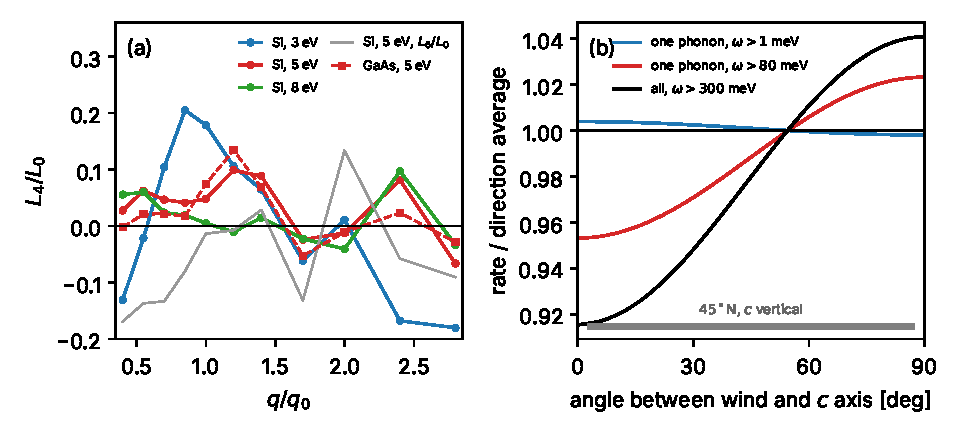
\includegraphics[width=\linewidth]{figures/ch11/fig11_7.pdf}
  \caption{Anisotropy of a cubic and of a uniaxial crystal. (a) Hexadecapole of the silicon loss function, the ratio $L_4/L_0$ of its components on the cubic harmonics $Y^{\mathrm{c}}_4$ and $Y^{\mathrm{c}}_0$, against $q/q_0$, $q_0 = \SI{3.73}{keV}$, at $\omega = 3$, 5 and \SI{8}{eV} (bins of \SI{1}{eV}); thin gray: $L_6/L_0$ at \SI{5}{eV}; dashed: GaAs at \SI{5}{eV}. Empirical pseudopotential model of \cref{sec:3.3}, head of the random-phase dielectric matrix, no local fields, ten directions of the irreducible wedge of the cube on a $k$ grid with the full cubic symmetry, components $\ell = 0$, 4, 6 and 8 fitted by least squares. (b) Rate of a sapphire crystal for a wind at a fixed angle to its $c$ axis, divided by the rate averaged over all wind directions, at $\mchi = \SI{10}{MeV}$ with a heavy mediator coupled to nucleon number: one phonon above \SI{1}{meV} (blue) and above \SI{80}{meV} (red), and all phonon numbers above \SI{300}{meV} (black). Incoherent nuclear response at $T = 0$ with the direction-dependent Debye--Waller exponents and projected densities of states of the published site tensors of Stratman and Lin~\cite{stratman2025daily}, whose $A_\kappa^2$-weighted anisotropy is $B^{cc}/B^{aa} - 1 = +0.059$. Bar: the range of angles swept in one sidereal day by a $c$ axis along the vertical at $45^\circ$N.}
  \label{fig:11-aniso}
\end{figure}

\Cref{fig:11-aniso}(b) shows the uniaxial case. Sapphire's rate depends on the direction of the wind almost only through the term $\ell = 2$, since the terms with $\ell \ge 4$ contribute less than $5\times10^{-4}$ of the rate, and its amplitude depends on which phonons the threshold admits. Above \SI{1}{meV}, where the acoustic and low optical phonons carry most of the one-phonon weight, the one-phonon rate along the axis and across it differ by \SI{0.6}{\percent}, and the rate of all phonon numbers by \SI{1.0}{\percent}, since these modes move all ten atoms of the cell almost isotropically. Above \SI{80}{meV} the highest optical modes alone remain, and they are polarized mostly in the basal plane: the one-phonon rate along the axis is \SI{7}{\percent} below the rate across it. Above \SI{300}{meV} the rate comes from three or more phonons, and \cref{eq:11.7-dw} multiplies the \SI{6}{\percent} anisotropy of the displacements by the phonon number: the difference grows to \SI{12}{\percent}. Mounted with its axis vertical at $45^\circ$N, a sapphire crystal then modulates with $A_{\mathrm{day}} = \SI{0.48}{\percent}$ for all phonons above \SI{1}{meV}, \SI{3.5}{\percent} for one phonon above \SI{80}{meV} and \SI{6.4}{\percent} above \SI{300}{meV}, at \SI{10}{MeV}. At \SI{30}{MeV} the amplitudes for the two higher thresholds fall to 1.2 and \SI{0.6}{\percent}. 2H-SiC, whose displacements are nearly isotropic, modulates less: 0.08, 0.61 and \SI{3.5}{\percent} for the same three cases at \SI{10}{MeV}. These are estimates within the incoherent approximation, which holds for $q$ above a few $q_{\mathrm{BZ}}$, here \SI{1.75}{keV} for the ten-atom cell of sapphire, and therefore for masses of a few MeV and above. They agree in pattern with the multiphonon calculation of Stratman and Lin, who find up to \SI{11}{\percent} in sapphire at \SI{10}{MeV} above \SI{300}{meV}, somewhat less in SiC and none in silicon and GaAs~\cite[Sect.~IV and App.~C]{stratman2025daily}. They use a different halo ($v_0 = 220$, $v_{\mathrm{esc}} = 500$ and $v_{\mathrm{E}} = \SI{240}{km.s^{-1}}$) and put the crystal axis along the wind at the start of the day. At lower masses the momentum transfers stay inside the zone, and the coherent single-phonon response decides the rate. The full phonon calculation of Griffin and collaborators finds daily modulation in sapphire of up to \SI{30}{\percent} at masses near \SI{50}{keV}, for a threshold that leaves only the optical branches. With the acoustic branches open it finds much less, because the sound speeds of sapphire are nearly isotropic~\cite[Sects.~III\,C and IV\,C]{griffin2018directional}. The same holds for the hexagonal polytypes of SiC, with the largest modulation in 2H~\cite[Sects.~IV\,B and V]{griffin2021sic}.

In silicon both the electron and the nucleon rates modulate, and with the same phase.

\begin{workedexample}{Daily modulation of a silicon crystal at $45^\circ$N}\label{we:11-daily}
A silicon crystal sits at latitude $45^\circ$N with [001] along the local vertical, [100] pointing east and [010] north. Dark matter of mass \SI{2}{MeV} scatters through a heavy mediator, either on electrons, through the loss function, or on nucleons, through the nuclear response. At this mass the momentum transfers reach $2\mchi v_{\mathrm{max}} = \SI{10.6}{keV} = 2.84\,q_0$; the electronic model ends at $2.8\,q_0$, and the sliver above it, at the kinematic edge where the rate vanishes, is dropped. The energy deposited on electrons stays below $\mchi v_{\mathrm{max}}^2/2 = \SI{7.0}{eV}$.

\emph{Geometry.} By \cref{eq:1.2-local}, the wind direction in crystal axes is
\begin{multline*}
  \hat{\vect{v}}_{\mathrm{E}} = \bigl(-\cos\delta_{\mathrm{E}}\sin h_{\mathrm{E}},\ \cos\ell_{\mathrm{lat}}\sin\delta_{\mathrm{E}} - \sin\ell_{\mathrm{lat}}\cos\delta_{\mathrm{E}}\cos h_{\mathrm{E}},\\
  \sin\ell_{\mathrm{lat}}\sin\delta_{\mathrm{E}} + \cos\ell_{\mathrm{lat}}\cos\delta_{\mathrm{E}}\cos h_{\mathrm{E}}\bigr) ,
\end{multline*}
with $\delta_{\mathrm{E}} = 47.5^\circ$ and the hour angle $h_{\mathrm{E}}$ advancing at the sidereal rate. Along this path $Y^{\mathrm{c}}_4$ of \cref{eq:C.3-cubic} runs from $-0.394$ to $0.640$, its maximum at $h_{\mathrm{E}} = 0$, when the wind arrives nearly along [001]. Let $\mathcal{R}_\ell$ be the term $\ell$ of \cref{eq:11.7-rate}, integrated over $q$ and $\omega$ without its factor $Y^{\mathrm{c}}_\ell$, and $\bar{\mathcal{R}}$ the rate averaged over orientations. If the hexadecapole dominates, $\mathcal{R}(t)/\bar{\mathcal{R}} = 1 + \sqrt{4\pi}\,(\mathcal{R}_4/\mathcal{R}_0)\,Y^{\mathrm{c}}_4(\hat{\vect{v}}_{\mathrm{E}}(t))$, and
\begin{equation*}
  A_{\mathrm{day}} = \sqrt{4\pi}\,\frac{0.640 + 0.394}{2}\,\frac{\mathcal{R}_4}{\mathcal{R}_0} = 1.83\,\frac{\mathcal{R}_4}{\mathcal{R}_0} .
\end{equation*}

\emph{Electronic part.} The integrals $\mathcal{R}_\ell = \sum_\omega\int\dd q\,q^3\mathcal{H}_\ell(\vmin)L_\ell(q,\omega)$ over the spectrum, with the components of \cref{fig:11-aniso}(a) in bins of \SI{1}{eV} from 1.5 to \SI{7.5}{eV}, give $\mathcal{R}_4/\mathcal{R}_0 = 4.9\times10^{-3}$, while $\mathcal{R}_6/\mathcal{R}_0 = -3\times10^{-5}$ and $\mathcal{R}_8/\mathcal{R}_0 = -7\times10^{-6}$ are negligible. The components beyond $\ell = 8$, which the ten directions do not resolve, enter with $\mathcal{H}_{10}$; estimated from the residual of the fit, they can shift the rate by about $10^{-3}$. The hexadecapole of the response, a few percent, passes because \SI{47}{\percent} of the rate of so light a particle comes from $\vmin > \SI{600}{km.s^{-1}}$, where the halo is sharp: weighted with the rate, $\mathcal{H}_4/\mathcal{H}_0$ is 0.09. The amplitude is $A_{\mathrm{day}} = 1.83\times4.9\times10^{-3} = \SI{0.9}{\percent}$, uncertain by about 0.1 percentage point from those higher components. The rate oscillates twice per sidereal day, with its maximum when Cygnus crosses the meridian.

\emph{Lattice part.} For the nucleon coupling, $\mathcal{R}_\ell = \sum_n\int\dd q\,q\,\mathcal{H}_\ell(q/2\mchi)\,\ee^{-2W}(2W)^n/n!\,s_{n,\ell}(q)$, with $2W = q^2\langle u_x^2\rangle$, $\langle u_x^2\rangle = \SI{2.45e-3}{\angstrom^2}$, and $s_{n,\ell}$ the cubic components of the exact one- and two-phonon weights of \cref{sec:11.3}, divided by their incoherent values; three and more phonons are treated as isotropic, their coherent corrections being below \SI{3}{\percent}. In $\vmin$ the deposit of $n$ phonons enters as $n\times\SI{30.4}{meV}/q$, the mean energy of the single-phonon distribution, which matters only at the smallest $q$, where the rate is small. The momentum transfers cross the shells $\vect{G}_{111}$ and $\vect{G}_{220}$, where the one-phonon weight is most anisotropic, and $\mathcal{R}_4/\mathcal{R}_0 = 3.2\times10^{-3}$, so $A_{\mathrm{day}} = \SI{0.58}{\percent}$, in phase with the electronic part since both $\mathcal{R}_4$ are positive. A detector that records both channels therefore sees an amplitude between 0.6 and \SI{0.9}{\percent}, the mean of the two weighted by their rates.

\emph{Mounting.} Over 3000 random orientations of the crystal at this latitude the largest amplitudes are 0.93 and \SI{0.60}{\percent}, so the vertical [001] is close to the best choice. With [001] along the Earth's axis instead, the wind circles at a fixed angle to [001], only the term $\cos4\varphi$ of $Y^{\mathrm{c}}_4$ varies, and the amplitudes drop to 0.15 and \SI{0.06}{\percent}, with four maxima per sidereal day.

\emph{GaAs.} The same mounting and mass give $\mathcal{R}_4/\mathcal{R}_0 = 3.8\times10^{-3}$ and $A_{\mathrm{day}} = \SI{0.7}{\percent}$ for the electronic part, in the same model and with the same uncertainty. For the nuclear part, with the one-phonon weights of the force constants of \cref{sec:5.5} and $\langle u_x^2\rangle \approx \SI{1.9e-3}{\angstrom^2}$, they give $\mathcal{R}_4/\mathcal{R}_0 = 1.6\times10^{-3}$ and $A_{\mathrm{day}} = \SI{0.29}{\percent}$. Both parts are in phase with those of silicon, and the combined amplitude of a GaAs detector lies between 0.3 and \SI{0.7}{\percent}.
\end{workedexample}

At \SI{1}{MeV}, where $2\mchi v_{\mathrm{max}} = \SI{5.3}{keV}$ lies just beyond the shell $\vect{G}_{111}$, the lattice amplitude of silicon is \SI{0.77}{\percent}, with the opposite phase, because $S_4$ is negative there. (Near $\vect{G}_{200}$ the two sublattices cancel, as for the Bragg peak, and the soft phonons add nothing.) At 0.7 and \SI{1.5}{MeV} the amplitude is only 0.13 and \SI{0.18}{\percent}. Each of these amplitudes is a product of an anisotropy of the response and the halo multipole of the same order. Cubic crystals, whose first term is $\ell = 4$, stay below about \SI{1}{\percent} in both sectors. Uniaxial crystals reach several percent, more for thresholds that select phonons polarized along one axis or the multiphonon tail, and at the lowest masses the coherent single-phonon response of a polar uniaxial crystal reaches tens of percent. Only near the kinematic edge does the halo pass every multipole, and a measurement there needs the full direction-resolved response.

\section{Absorption on phonons and acoustic modes}\label{sec:11.8}

A dark photon of mass \SI{36.35}{meV} that is absorbed in GaAs deposits its whole energy in one longitudinal optical phonon, and its momentum, $m_\phi v \approx \SI{46}{\micro eV}$, is a part in $10^{8}$ of the zone. Absorption samples the crystal at a single point, $\vect{q} = \vect{p}_\phi$ and $\omega = m_\phi$ (\cref{sec:8.2-absorption}), and below the electronic gap the only excitations at that point are the optical phonons at the zone center. For bosons of a neV or a \si{\micro eV} the picture changes again. Their de Broglie wavelength $2\pi/m_\phi v$, a kilometer at \SI{1}{\micro eV}, is larger than any detector, and the field is a classical wave that oscillates in phase over the whole body. What absorbs it is a normal mode of the body itself, at MHz in a millimeter crystal and at kHz in a ton-scale bar. A scalar coupled to electrons sees the electrons that a longitudinal phonon carries with each nucleus, and in GaAs, where the two sublattices carry nearly equal numbers per unit mass, its rate is a near-cancellation.

\subsection{Single-phonon absorption}\label{sec:11.8-single}

The absorption rate per quantum is the master formula \cref{eq:8.2-abs} at one point. Collect the couplings of the field into one row, $O_\phi = \sum_ag^\phi_aO_a(\vect{p}_\phi)$; then $\varGamma_{\mathrm{abs}} = S_{O_\phi O_\phi}(\vect{p}_\phi,\omega_\phi)/2\omega_\phi$, and in a cold insulator below the gap $S$ is the one-phonon structure factor. The kinematics leaves no choice of branch. An acoustic phonon of momentum $p_\phi$ has the energy $c_\nu p_\phi = c_\nu v\,m_\phi$, and absorbing the boson would need $c_\nu v = 1$, while sound speeds are $\sim 10^{-5}$ and $v \sim 10^{-3}$ in units of the speed of light. An optical phonon at $\vect{Q} = \vect{p}_\phi$ is the zone-center phonon to a part in $10^{15}$, since the dispersion starts at order $(p_\phi a)^2$. The momentum transfer is far below the \SI{0.05}{eV} at which the finite-$q$ structure of the longitudinal mode becomes visible (\cref{we:8-nucleon}), and the zone-center vertex is exact here. The finite-$q$ corrections of \cref{sec:11.2}, the piezoelectric charge of the acoustic branches and the dynamical quadrupoles, play no role.

For a row built from densities the one-phonon structure factor has the form of \cref{eq:11.1-S1} and \cref{eq:11.2-SZZ}: each sublattice contributes its displacement projected on $\vect{p}_\phi$, times a coupling per site. With $\omega_\phi \simeq m_\phi$ and $T = 0$,
\begin{equation}
  \varGamma_{\mathrm{abs}} = \frac{\pi}{2\Omega\,m_\phi}\sum_\nu\frac{\bigl|\sum_\kappa\vect{p}_\phi\cdot\mathcal{G}^\phi_\kappa\cdot\vect{e}_{\kappa\nu}(0)^*/\sqrt{M_\kappa}\bigr|^2}{\omega_\nu}\;\delta(m_\phi - \omega_\nu) ,
  \label{eq:11.8-Gamma}
\end{equation}
with $\omega_\nu$ and $\vect{e}_{\kappa\nu}(0)$ the zone-center phonons of the full dynamical matrix for the direction $\hat{\vect{p}}_\phi$, nonanalytic term included. The tensor $\mathcal{G}^\phi_\kappa$ is the coupling of the field to the motion of site $\kappa$, and finding it is the whole problem. The naive answer is the coefficient of each species times the number of particles that move with the nucleus. For the nucleons that number is fixed. For the electrons it is not, because how many electrons follow a nucleus depends on the macroscopic field that the motion itself creates.

The Born charge answers half of the question. By its definition in \cref{sec:5.5}, $Z^*_\kappa$ is the charge that moves with nucleus $\kappa$ at zero macroscopic field: the nuclear charge $Z_\kappa$ minus the electrons that follow. At zero field the electrons that follow thus number $Z_\kappa\mathbb{1} - Z^*_\kappa$, and this is the vertex of the electron density in the proper response. A longitudinal phonon, however, carries a macroscopic field, and the electrons respond to it as well. The screened response \cref{eq:8.4-rank1} adds that field, and \cref{we:8-nucleon} has done the algebra for a nucleon row. The electron row differs in one respect: it also correlates with the charge through the electrons alone, at fixed nuclei.

For any pair of rows, take frequencies near the optical phonons and neglect local fields. The screened response is then the rank-one form \cref{eq:8.4-rank1}, $R_{ab} = \tilde R_{ab} + v_{\mathrm{C}}\tilde R_{aZ}\tilde R_{Zb}/\varepsilon$ with $\varepsilon = 1 - v_{\mathrm{C}}\tilde R_{ZZ}$, built from the proper responses $\tilde R$. The proper response of rows $a$ and $b$ then has a phonon part and an electronic part,
\begin{equation*}
  \tilde R_{ab} = \frac{q^2}{\Omega}\,\vect{p}_a^{\mathrm{T}}\bigl(\omega^2 - D^{\mathrm{an}}\bigr)^{-1}\vect{p}_b + \chi_{ab} ,
\end{equation*}
with $\vect{p}_a$ the $3n$-vector of the proper site couplings of row $a$ divided by $\sqrt{M_\kappa}$ and projected on $\hat{\vect{q}}$, as in \cref{eq:11.2-eps}, and $\chi_{ab}$ the real response of the electrons at clamped nuclei. For the charge row, $\vect{p}_Z = \vect{p}$ is built from the Born charges and $v_{\mathrm{C}}\chi_{ZZ} = 1 - \varepsilon_\infty$. Write $x_a = (q^2/\Omega)\,\vect{p}_a^{\mathrm{T}}(\omega^2 - D^{\mathrm{an}})^{-1}\vect{p}$ and $x = x_Z$, so that $\varepsilon = \varepsilon_\infty - v_{\mathrm{C}}x$. The full phonon propagator $(\omega^2 - D^{\mathrm{an}} - \vect{b}\vect{b}^{\mathrm{T}})^{-1}$, with $\vect{b}\vect{b}^{\mathrm{T}}$ the nonanalytic term of \cref{eq:11.2-SM}, follows from the Sherman--Morrison identity, and between rows it gives $x_ax_b$-type terms:
\begin{equation*}
  \frac{q^2}{\Omega}\,\vect{p}_a^{\mathrm{T}}\bigl(\omega^2 - D^{\mathrm{an}} - \vect{b}\vect{b}^{\mathrm{T}}\bigr)^{-1}\vect{p}_b = \frac{q^2}{\Omega}\,\vect{p}_a^{\mathrm{T}}\bigl(\omega^2 - D^{\mathrm{an}}\bigr)^{-1}\vect{p}_b + \frac{v_{\mathrm{C}}\,x_ax_b}{\varepsilon_\infty - v_{\mathrm{C}}x} .
\end{equation*}
Insert $\tilde R_{aZ} = x_a + \chi_{aZ}$ into \cref{eq:8.4-rank1} and expand the product $(x_a + \chi_{aZ})(x_b + \chi_{bZ})$. The $x_ax_b$ term is the one just written. The terms linear in $\chi$ and the $\chi\chi$ term are reproduced by shifting each vertex by $\lambda_a\vect{p}$ with $\lambda_a = v_{\mathrm{C}}\chi_{aZ}/\varepsilon_\infty$, since $(q^2/\Omega)\vect{p}_a^{\mathrm{T}}(\omega^2 - D^{\mathrm{an}} - \vect{b}\vect{b}^{\mathrm{T}})^{-1}\vect{p} = \varepsilon_\infty x_a/\varepsilon$ by the same identity; what remains of the $\chi\chi$ term is a real constant. The result is exact within the rank-one form:
\begin{equation}
  R_{ab} = \frac{q^2}{\Omega}\,\vect{p}'^{\mathrm{T}}_a\bigl(\omega^2 - D^{\mathrm{an}} - \vect{b}\vect{b}^{\mathrm{T}}\bigr)^{-1}\vect{p}'_b + \chi_{ab} + \frac{v_{\mathrm{C}}\chi_{aZ}\chi_{Zb}}{\varepsilon_\infty} ,
  \qquad \vect{p}'_a = \vect{p}_a + \frac{v_{\mathrm{C}}\chi_{aZ}}{\varepsilon_\infty}\,\vect{p} .
  \label{eq:11.8-shift}
\end{equation}
The transverse poles are gone, the phonons are those of the full dynamical matrix, and each row keeps its own vertex, shifted along the Born-charge vector by its electronic correlation with the charge. The constant is real and does not absorb. For the electron density, $n_Z = -n_e + \sum_\kappa Z_\kappa n_\kappa$ gives $\chi_{eZ} = -\chi_{ee} = -\chi_{ZZ}$, so that $v_{\mathrm{C}}\chi_{eZ} = \varepsilon_\infty - 1$, and the shift adds $(1 - 1/\varepsilon_\infty)Z^*_\kappa$ to the proper vertex $Z_\kappa\mathbb{1} - Z^*_\kappa$.
\begin{keyresult}[Site coupling of a density row at the longitudinal pole]
A field that couples to $\sum_\kappa g^\phi_{n_\kappa}n_\kappa + g^\phi_{n_e}n_e$ creates the zone-center phonons of \cref{eq:11.8-Gamma} with the site couplings
\begin{equation}
  \mathcal{G}^\phi_\kappa = g^\phi_{n_\kappa}\mathbb{1} + g^\phi_{n_e}\Bigl(Z_\kappa\mathbb{1} - \frac{Z^*_\kappa}{\varepsilon_\infty(\hat{\vect{p}}_\phi)}\Bigr) ,
  \label{eq:11.8-G}
\end{equation}
for $\omega$ far below the gap, without local fields, and in the harmonic lattice. A longitudinal phonon carries $Z_\kappa - Z^*_\kappa/\varepsilon_\infty$ electrons with nucleus $\kappa$.
\end{keyresult}
\noindent The total charge, the nucleon number and the electron density each test \cref{eq:11.8-G}. For the total charge, $g^\phi_{n_e} = -\lambda$ and $g^\phi_{n_\kappa} = \lambda Z_\kappa$, and the nuclear charge cancels to leave $\lambda Z^*_\kappa/\varepsilon_\infty$, the screened Born charge of \cref{eq:11.2-SZZ}. For the nucleons, $g^\phi_{n_e} = 0$ and the vertex is the bare coefficient, unscreened, as \cref{we:8-nucleon} found. For the electrons alone the vertex is new. In the longitudinal wave the macroscopic field is $-\vect{P}/\varepsilon_\infty$, the electrons polarize in it, and they move another $Z^*_\kappa(1 - 1/\varepsilon_\infty)$ along with the nucleus, in addition to the $Z_\kappa - Z^*_\kappa$ that follow at zero field.

Optical phonons do not move the center of mass, $\sum_\kappa\sqrt{M_\kappa}\,\vect{e}_{\kappa\nu}(0) = 0$, and by the coupling-to-mass cancellation of \cref{sec:11.6-random} the sum in \cref{eq:11.8-Gamma} is unchanged when $\mathcal{G}^\phi_\kappa \to \mathcal{G}^\phi_\kappa - \lambda M_\kappa\mathbb{1}$ for any $\lambda$: a coupling proportional to the mass excites no optical phonon at all~\cite[Eq.~(44)]{mitridate2024effective}. What \cref{eq:11.8-Gamma} measures is how far the site couplings deviate from proportionality to the masses. For two atoms in the cell, with the longitudinal eigenvector of \cref{sec:11.2}, $\vect{e}_1 = (M_2/M_{\mathrm{cell}})^{1/2}\hat{\vect{p}}_\phi$ and $\vect{e}_2 = -(M_1/M_{\mathrm{cell}})^{1/2}\hat{\vect{p}}_\phi$, the sum collapses to $p_\phi\,\mu_{\mathrm{red}}^{1/2}\,d$ with the mass-weighted difference
\begin{equation}
  d = \frac{\mathcal{G}^\phi_1}{M_1} - \frac{\mathcal{G}^\phi_2}{M_2} ,
  \label{eq:11.8-d}
\end{equation}
in a cubic crystal, where the tensors are scalars. Only the longitudinal mode couples, since $\vect{p}_\phi\cdot\vect{e}$ vanishes for the transverse ones.

The rate takes a compact form through the loss function. By \cref{eq:11.2-onebranch} the longitudinal line of $L$ has the weight $\pi e^2Z^{*2}/(2\Omega\mu_{\mathrm{red}}\varepsilon_\infty^2\omega_{\mathrm{L}})$. Dividing \cref{eq:11.8-Gamma} by it, averaging $p_\phi^2 = m_\phi^2v^2$ over the halo and multiplying by $\rho_\chi/m_\phi\rho_T$,
\begin{equation}
  \mathcal{R} = \frac{\rho_\chi}{\rho_T}\,\frac{\langle v^2\rangle}{e^2}\Bigl(\frac{\varepsilon_\infty\,\mu_{\mathrm{red}}\,d}{Z^*}\Bigr)^2L(m_\phi) .
  \label{eq:11.8-Rscalar}
\end{equation}
In the one-branch crystal, with the damping carried by the phonon propagator, \cref{eq:11.8-shift} makes the full response of any density row proportional to $L(\omega)$ at every frequency, not only at the pole. The line shape is that of the loss function, peaked at $\omega_{\mathrm{L}}$, with no feature at $\omega_{\mathrm{T}}$. For a coupling proportional to the charge the bracket is one, and \cref{eq:11.8-Rscalar} is the photon-like rate of Mitridate and collaborators~\cite[Eq.~(42)]{mitridate2024effective}. Compared with the dark photon below, it carries $\langle v^2\rangle$, since a scalar couples to a density, whose matrix elements vanish as $p_\phi \to 0$. For the standard halo of \cref{sec:1.2}, $\langle v^2\rangle^{1/2} = \SI{379}{km/s}$. A photon-like scalar then reaches the dark-photon sensitivity at $g = \zeta e/\langle v^2\rangle^{1/2} = 240\,\zeta$.

For a scalar that couples to nucleon number the bracket is $\varepsilon_\infty\mu_{\mathrm{red}}d_N/Z^*$, with $d_N$ the difference of nucleon number per mass between the two species, $2.6\times10^{-5}$ per u in GaAs (\cref{we:8-nucleon}). The bracket is $4.8\times10^{-3}$, and the rate is $2\times10^{-5}$ of the photon-like one. Masses are nearly proportional to nucleon numbers, and the coupling-to-mass cancellation is nearly complete. In a crystal of mixed isotopes the cancellation fails site by site, the translation symmetry that selects the zone center is broken, and the absorption spreads over the whole phonon band (\cref{sec:11.6}).

A dark photon does not couple to a density. At rest it couples to the current, with any of three polarizations, and its rate per particle is $\varGamma_{\mathrm{net}} = \zeta^2m_\phi L(m_\phi)$ with the total dielectric function (\cref{sec:10.7-darkphoton}), the loss function again, now without the factor $v^2$. Why a transverse field excites the longitudinal phonon is the physics of the phonon polariton (\cref{sec:5.5}). The photon of the crystal and its transverse optical phonon mix into two branches near $Q \sim \varepsilon_0^{1/2}\omega_{\mathrm{T}}$, about \SI{0.12}{eV} in GaAs. The upper branch starts at $Q = 0$ at the zero of $\varepsilon$, which is $\omega_{\mathrm{L}}$; the lower one starts at zero frequency. The dark photon sits at $Q = p_\phi$, some 2600 times below the crossover, where the upper branch is flat at $\omega_{\mathrm{L}}$ and the distinction between transverse and longitudinal has disappeared: at $Q \to 0$ a cubic crystal has $\varepsilon^{\mathrm{T}} = \varepsilon$ (\cref{eq:4.4-ET}). With the line of \cref{eq:11.2-Ipol}, the rate integrated over the mass is
\begin{equation}
  \int\dd m_\phi\;\mathcal{R} = \frac{\rho_\chi}{\rho_T}\,\zeta^2\,\mathcal{I}_{\mathrm{pol}} ,
  \label{eq:11.8-Rint}
\end{equation}
the band integral of \cref{sec:11.2}, independent of the widths of the lines. Dark-photon absorption is single-phonon scattering through a dark photon, read at $q \to 0$.

\begin{limitbox}[Single-phonon absorption][lim:11.8a]
A boson absorbed on optical phonons has the rate $\varGamma_{\mathrm{abs}} = (\pi/2\Omega m_\phi)\sum_\nu|\sum_\kappa\vect{p}_\phi\cdot\mathcal{G}^\phi_\kappa\cdot\vect{e}^*_{\kappa\nu}(0)/\sqrt{M_\kappa}|^2\delta(m_\phi - \omega_\nu)/\omega_\nu$, \cref{eq:11.8-Gamma}~\cite[Eqs.~(2), (7), (14), (16)]{mitridate2024effective}. For a dark photon it is $\mathcal{R} = (\rho_\chi/\rho_T)\zeta^2\,\Imag[-1/\varepsilon(m_\phi)]$~\cite[Eqs.~(2), (3)]{knapen2018detection}, and for scalars \cref{eq:11.8-Rscalar} with the site couplings \cref{eq:11.8-G}.
\par\smallskip
{\centering
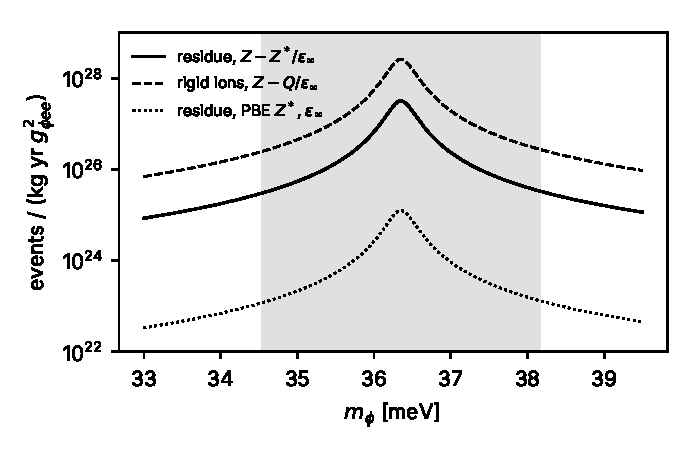
\includegraphics[width=0.8\linewidth]{figures/ch11/limit11_8a.pdf}
\captionof{figure}{Absorption of a scalar coupled to electrons in GaAs, events per kilogram-year and per $g_{\phi ee}^2$, against $m_\phi$, from \cref{eq:11.8-Rscalar}. Solid: site couplings $Z_\kappa - Z^*_\kappa/\varepsilon_\infty$ with $Z^* = 2.11$ and $\varepsilon_\infty = 10.88$ (\cref{we:5-lst}); a change of $Z^*/\varepsilon_\infty$ by $\pm\SI{1}{\percent}$ moves it by $\pm9\,\%$, less than the width of the line on this scale. Dotted: site couplings $Z_\kappa - Z^*_\kappa/\varepsilon_\infty$ with the PBE values $Z^* = 2.094$ and $\varepsilon_\infty = 13.70$ of \cref{sec:5.5}, 250 times lower. Loss function of one damped branch with $\omega_{\mathrm{T}} = 33.62$, $\omega_{\mathrm{L}} = \SI{36.35}{meV}$ and widths set to \SI{1}{\percent} of each frequency~\cite[Sect.~III\,A]{mitridate2024effective}; standard halo of \cref{sec:1.2}, $\langle v^2\rangle^{1/2} = \SI{379}{km/s}$, $\rho_T = \SI{5.361}{g.cm^{-3}}$. Gray: $|m_\phi - \omega_{\mathrm{L}}| < 5\gamma_{\mathrm{L}}$, where a line of constant width describes the phonon.}\label{fig:11-limit-8a}
\par}
\smallskip
Where the mass-weighted difference $d$ is small against each of its terms, the corrections that \cref{eq:11.8-G} drops are no longer small against the rate, and the formula fixes only its order of magnitude.
\end{limitbox}

\subsection{The near-cancellation in GaAs}\label{sec:11.8-gaas}

A scalar that couples to electrons through $g_{\phi ee}$ acts on the row $-g_{\phi ee}n_e$ (\cref{eq:8.1-scalar}), so that $g^\phi_{n_e} = -g_{\phi ee}$ and $g^\phi_{n_\kappa} = 0$, and by \cref{eq:11.8-G} each site contributes $Z_\kappa - Z^*_\kappa/\varepsilon_\infty$ electrons. GaAs is the obvious target, polar and well measured, and it turns out to be close to the worst case.

\begin{workedexample}{The electron-coupled scalar in GaAs}\label{we:11-gaas}
We take the inputs of \cref{sec:11.2}: $Z^* = 2.11$ from the splitting and the measured $\varepsilon_\infty = 10.88$, so that $Z^*/\varepsilon_\infty = 0.1939$, with $Z^*_{\mathrm{Ga}} = +Z^*$ and $Z^*_{\mathrm{As}} = -Z^*$; atomic numbers 31 and 33; mean atomic masses \SI{69.723}{u} and \SI{74.9216}{u}; $\mu_{\mathrm{red}} = \SI{36.11}{u}$.

\emph{Site couplings.} Gallium carries $31 - 0.1939 = 30.806$ electrons and arsenic $33 + 0.1939 = 33.194$, and each site couples with $-g_{\phi ee}$ times its count.

\emph{Mass-weighted difference.} Split \cref{eq:11.8-d} into its two parts. The nuclear charges per unit mass are $Z_{\mathrm{Ga}}/M_{\mathrm{Ga}} = 0.44462$ and $Z_{\mathrm{As}}/M_{\mathrm{As}} = 0.44046$ per u, and their difference is $+4.16\times10^{-3}$. The Born charges contribute $-(Z^*/\varepsilon_\infty)(1/M_{\mathrm{Ga}} + 1/M_{\mathrm{As}}) = -0.1939 \times 0.02769 = -5.37\times10^{-3}$. The sum is $d = -1.21\times10^{-3}$ per u, times $-g_{\phi ee}$. The two terms are 3.4 and 4.4 times larger than their sum.

\emph{Rate.} The bracket of \cref{eq:11.8-Rscalar} is $\varepsilon_\infty\mu_{\mathrm{red}}d/Z^* = 10.88 \times 36.11 \times 1.214\times10^{-3}/2.11 = 0.226$, and its square is $0.051$. An electron-coupled scalar is absorbed in GaAs at \SI{5}{\percent} of the rate of a photon-like scalar of the same coupling.

\emph{Sensitivity.} Since the Born-charge term is 4.4 times $|d|$, a fractional change of $Z^*/\varepsilon_\infty$ changes $d$ 4.4 times as much and the rate 8.8 times as much. The splitting route of \cref{sec:11.2-split} fixes $Z^*/\varepsilon_\infty$ to \SI{1.0}{\percent}, and these inputs limit the rate to \SI{9}{\percent}. Exact cancellation would need $Z^*/\varepsilon_\infty = 0.1501$. The values $Z^* = 2.16$ and $\varepsilon_\infty = 10.9$, also found in the literature, would give $d = -1.33\times10^{-3}$, a rate \SI{20}{\percent} higher.
\end{workedexample}

At the line center, with widths of \SI{1}{\percent}, three events in a kilogram-year need $g_{\phi ee} = 3.1\times10^{-14}$. III--V crystals, whose neighbors in the periodic table have nearly equal charge per mass, suppress the absorption of an electron-coupled scalar.

The kinetic energy of the core electrons, the isotopic masses and the frequency dependence of the electronic response are left out of \cref{eq:11.8-G}; each is small in absolute terms but not against $d$. The scalar density of an electron is its number density times $1 - v^2/2$ (\cref{eq:8.1-scalar}), and the core electrons that ride with a nucleus move fast. Their kinetic-energy row enters through the same factor $\ii\vect{p}_\phi\cdot\vect{u}_\kappa$ as their density, and it reduces the electrons each site carries by $\langle\mathcal{T}\rangle_\kappa/m_e$, the kinetic energy of those electrons over the electron mass. By the virial theorem this is the binding energy of the atom over $m_e$, tens of keV over \SI{511}{keV}, of order 0.1 for gallium and arsenic. As a parametric estimate, its mass-weighted difference between the two sites is $\Delta d \approx +1.2\times10^{-4}$ per u, a tenth of $d$ and of the opposite sign, so that it lowers $|d|$ by about \SI{10}{\percent} and the rate by about \SI{19}{\percent}. No calculation has included it yet, and \cref{sec:11.9} carries it as a nuisance. The masses enter at the same level: \SI{0.01}{u} on the mean mass of gallium moves $d$ by \SI{5}{\percent}, so an isotopically enriched crystal must use its own masses. The frequency dependence of the electronic response, of relative order $(\omega_{\mathrm{L}}/\Eg)^2 = 6\times10^{-4}$ (\cref{sec:11.2}), is amplified by 4.4 to \SI{0.3}{\percent} of $d$ and is negligible.

Density-functional perturbation theory delivers $Z^*$ robustly, to a percent, and $\varepsilon_\infty$ poorly. With the PBE values of \cref{sec:5.5}, $Z^* = 2.094$ and $\varepsilon_\infty = 13.70$, the ratio $Z^*/\varepsilon_\infty = 0.153$ lies within \SI{2}{\percent} of exact cancellation, $d = -7.6\times10^{-5}$ per u, and the rate falls by a factor of 250 (the dotted curve of \cref{lim:11.8a}). The test of the computed values against the measured splitting, \cref{eq:E.4-LOTO}, matters more here than any convergence parameter, and the measured splitting with \cref{eq:11.2-Zeps} is the safer input; the phonon widths come from three-phonon perturbation theory (\cref{sec:5.7}).

\subsection{Dark photons in GaAs and sapphire}\label{sec:11.8-dp}

For a dark photon the vertex is the screened Born charge, there is no cancellation, and the rate is the measured or computed loss function, $\mathcal{R} = (\rho_\chi/\rho_T)\zeta^2L(m_\phi)$ (\cref{eq:10.7-dp}). Two numbers characterize each line: its area, which is fixed by the band integral \cref{eq:11.8-Rint}, and its width, which is not. For GaAs, $\mathcal{I}_{\mathrm{pol}} = \SI{0.759}{meV}$ from the splitting (\cref{we:11-ipol}), and a Lorentzian of full width $\gamma_{\mathrm{L}}$ peaks at $L = 2\mathcal{I}_{\mathrm{pol}}/\pi\gamma_{\mathrm{L}}$. A width of \SI{1}{\percent} of the frequency leads to $L = 1.33$ at the center, ten times narrower gives 13.3, and the area stays at \SI{0.76}{meV}. The reach on the line center scales as $\gamma_{\mathrm{L}}^{1/2}$, while the reach averaged over a scan of masses depends only on the area.

\begin{figure}[tbp]
  \centering
  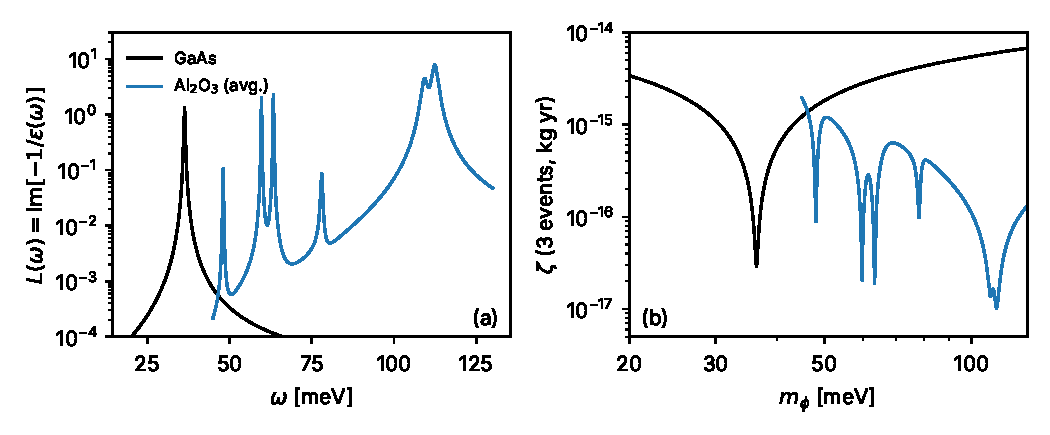
\includegraphics[width=\linewidth]{figures/ch11/fig11_8.pdf}
  \caption{Absorption of dark-photon dark matter on single optical phonons. (a) Loss function $L = \Imag[-1/\varepsilon(\omega)]$ at $q \to 0$ from the damped factorized dielectric function $\varepsilon_\infty\prod_\nu(\omega_{\mathrm{L}\nu}^2 - \omega^2 - \ii\omega\gamma_{\mathrm{L}\nu})/(\omega_{\mathrm{T}\nu}^2 - \omega^2 - \ii\omega\gamma_{\mathrm{T}\nu})$. GaAs (black): $\omega_{\mathrm{T}} = 33.62$, $\omega_{\mathrm{L}} = \SI{36.35}{meV}$, $\varepsilon_\infty = 10.88$, so that the line carries the splitting weight $(1 - \omega_{\mathrm{T}}^2/\omega_{\mathrm{L}}^2)/\varepsilon_\infty = 0.0133$ (\cref{sec:11.2}), with an assumed width of \SI{1}{\percent} of each frequency. Sapphire (blue): the frequencies and \SI{77}{K} widths of Ref.~\cite[Table~II]{griffin2018directional} for the ordinary and extraordinary rays, as listed in \cref{lim:10.7a}, and $\varepsilon_\infty = 3.2$; averaged over polarizations as $\frac23L_{\mathrm{o}} + \frac13L_{\mathrm{e}}$~\cite[Eq.~(40)]{griffin2018directional}; drawn above \SI{45}{meV}, since below the lowest transverse line the model gives $|L| < 10^{-4}$ of the wrong sign. (b) Kinetic mixing $\zeta$ for three events in one kilogram-year without background, $\mathcal{R} = (\rho_\chi/\rho_T)\zeta^2L(m_\phi)$, with $\rho_\chi = \SI{0.3}{GeV.cm^{-3}}$ and $\rho_T = 5.361$ and \SI{3.98}{g.cm^{-3}}. Single-phonon lines only: the multiphonon absorption between them and the electronic absorption above the gap are not included.}
  \label{fig:11-dpabs}
\end{figure}

\Cref{fig:11-dpabs} shows both crystals. GaAs has one line, and three events in a kilogram-year reach $\zeta = 2.9\times10^{-17}$ at its center. Sapphire has six polar branches between the two polarizations. The strongest is the collective top branch of the ordinary ray, at \SI{112.4}{meV}, which carries \SI{95}{\percent} of the ordinary weight (\cref{sec:11.2-band}). With its measured \SI{77}{K} width of \SI{2.0}{meV} it reaches $\zeta = 1.0\times10^{-17}$, and the lines at 59.7 and \SI{63.3}{meV} reach $2\times10^{-17}$. Per unit mass the band integral of sapphire is 64 times that of GaAs, $\SI{35.9}{meV}/\SI{3.98}{g.cm^{-3}}$ against $\SI{0.759}{meV}/\SI{5.361}{g.cm^{-3}}$; here \SI{35.9}{meV} is the polarization average $\frac23$ ordinary $+ \frac13$ extraordinary of the absorbed field, while the ordinary ray alone gives the \SI{36.3}{meV} of \cref{sec:11.2-band}. The widths are the weak input. Those of sapphire were measured at \SI{77}{K}, and at millikelvin temperatures the anharmonic part, the thermal part of \cref{eq:5.7-gamma}, shrinks while the spontaneous decay stays, so the lines should narrow by a factor of order one~\cite{griffin2018directional}. Between the lines the absorption is multiphonon, which the measured $\varepsilon$ contains and the factorized model does not, and it fills the gaps of \cref{fig:11-dpabs}b~\cite{knapen2018detection,griffin2018directional}.

\subsection{Acoustic modes of a finite body}\label{sec:11.8-bar}

The lowest thickness mode of a quartz plate \SI{1}{mm} thick rings at about \SI{3}{MHz}, an energy of \SI{12}{neV}. A dark photon of that mass has a de Broglie wavelength of order \SI{100}{km} and stays coherent for a fraction of a second, $t_{\mathrm{coh}} = 1/m_\phi v_0^2$, which is \SI{1.04}{ms} at \SI{1}{\micro eV} and scales as $1/m_\phi$. Even the wavelength of light at its frequency, $2\pi/m_\phi$, is \SI{100}{m}. Over the plate and over many periods the field is one classical wave, $\phi \propto \cos(m_\phi t)$, uniform in space. Crystal momentum no longer selects anything: a body small against the wavelength has no translation symmetry at that scale, and the role of $\vect{p}_\phi$ passes to the shape of the normal modes of the body. The acoustic modes, which could not absorb in an infinite crystal, now can, because a finite body has acoustic modes at nonzero frequency at zero wavevector of the field.

\emph{The field inside the body.} A dark photon at rest acts on charges as an electric field $\zeta\vect{E}'$, with $|\vect{E}'| = m_\phi|A'| = (2\rho_\chi)^{1/2}$ since $\rho_\chi = m_\phi^2|A'|^2/2$. In an infinite medium the induced polarization screens it to $\zeta\vect{E}'/\varepsilon$, the in-medium mixing of \cref{eq:8.4-zetaeff}. A body of size $L_{\mathrm{s}} \ll 2\pi/m_\phi$ is in the quasi-static regime, and its surface charges set the field instead. Take an ellipsoid with depolarization factor $N_{\mathrm{dp}}$ along the field. The induced polarization $(\varepsilon_0 - 1)\vect{E}_{\mathrm{in}}$ produces the depolarizing field $-N_{\mathrm{dp}}(\varepsilon_0 - 1)\vect{E}_{\mathrm{in}}$, so that $\vect{E}_{\mathrm{in}} = \zeta\vect{E}' - N_{\mathrm{dp}}(\varepsilon_0 - 1)\vect{E}_{\mathrm{in}}$, or
\begin{equation}
  \vect{E}_{\mathrm{in}} = \frac{\zeta\vect{E}'}{1 + N_{\mathrm{dp}}(\varepsilon_0 - 1)} = f_{\mathrm{sh}}\,\frac{\zeta\vect{E}'}{\varepsilon_0} ,
  \qquad f_{\mathrm{sh}} = 1,\ \ \frac{3\varepsilon_0}{\varepsilon_0 + 2},\ \ \varepsilon_0 ,
  \label{eq:11.8-shape}
\end{equation}
for a field normal to a slab ($N_{\mathrm{dp}} = 1$), in a sphere ($N_{\mathrm{dp}} = 1/3$) and parallel to a slab ($N_{\mathrm{dp}} = 0$). The static constant $\varepsilon_0$ appears because MHz frequencies lie far below the optical phonons. The slab with the field along its normal coincides with the bulk, and a field along a thin plate is not screened at all. A conducting shield of size $R_{\mathrm{s}}$ around the experiment suppresses the field further by $\min\{1, (m_\phi R_{\mathrm{s}})^2\}$~\cite[Eq.~(5)]{trickle2025piezoelectric}.

\emph{The coupling.} In a piezoelectric crystal a strain $S_{\beta\gamma}$ polarizes the cell, $P_\alpha = \sum_{\beta\gamma}e^{\mathrm{pz}}_{\alpha\beta\gamma}S_{\beta\gamma}$ (\cref{sec:6.2}), and the field couples through $\delta H = -\int\dd^3x\,\vect{E}_{\mathrm{in}}\cdot\vect{P}$. We take a plate cut so that its axis $z$ carries the dominant element, $e^{\mathrm{pz}} \equiv e^{\mathrm{pz}}_{zzz}$, and a field component $E_{\mathrm{in}}\cos\theta$ along $z$, with $\theta$ the angle between the polarization of the dark photon and the axis. Then $\delta H = -E_{\mathrm{in}}\cos\theta\,\cos(m_\phi t)\,e^{\mathrm{pz}}\int\dd^3x\,\partial_zu_z$.

\emph{The modes.} The displacement of the body is $\vect{u}(\vect{x}) = \sum_n\vect{U}_n(\vect{x})(b_n + b_n^\dagger)$, with the mode functions normalized as $\int\dd^3x\,\rho_T\,\vect{U}_n\cdot\vect{U}_{n'} = \delta_{nn'}/2\omega_n$, the finite-body form of \cref{eq:5.3-u}. A plano-convex plate of central thickness $L_0$ traps its thickness modes near the axis. Across it they have a Gaussian profile of radius $r_n$~\cite[Eqs.~(2), (3)]{trickle2025piezoelectric},
\begin{equation*}
  \vect{U}_n = \frac{\hat{\vect{z}}}{\sqrt{M_n\omega_n}}\,\cos\frac{n\pi z}{L_0}\,\exp\Bigl(-\frac{x^2 + y^2}{2r_n^2}\Bigr) ,
  \qquad M_n = \rho_T\pi r_n^2L_0 ,
  \qquad \omega_n = \frac{n\pi c_{\mathrm{L}}}{L_0} ,
\end{equation*}
which satisfies the normalization, since the cosine squared averages to one half and the Gaussian squared integrates to $\pi r_n^2$; $M_n$ is the mass of the mode and $c_{\mathrm{L}}$ the longitudinal sound speed of the plate. The polarization integral is
\begin{equation*}
  \int\dd^3x\,\partial_zU_{n,z} = \frac{\cos n\pi - 1}{\sqrt{M_n\omega_n}}\int\dd x\,\dd y\,\ee^{-(x^2 + y^2)/2r_n^2} = -\frac{4\pi r_n^2}{\sqrt{M_n\omega_n}} ,
\end{equation*}
for odd $n$, and zero for even $n$, whose two faces move together and leave no net polarization.

\emph{The power.} Write $\cos(m_\phi t) = (\ee^{-\ii m_\phi t} + \ee^{\ii m_\phi t})/2$ and keep the part $\delta H_0\,\ee^{-\ii m_\phi t}$ that absorbs. With $E_0 = f_{\mathrm{sh}}\zeta(2\rho_\chi)^{1/2}/\varepsilon_0$ the amplitude of $E_{\mathrm{in}}$ and $\pi r_n^2 = M_n/\rho_TL_0$,
\begin{equation*}
  |\langle n|\delta H_0|0\rangle|^2 = \Bigl(\frac{E_0\cos\theta\,e^{\mathrm{pz}}}{2}\Bigr)^2\frac{16\pi^2r_n^4}{M_n\omega_n}
  = \frac{8f_{\mathrm{sh}}^2\zeta^2\rho_\chi(e^{\mathrm{pz}})^2M_n\cos^2\theta}{\varepsilon_0^2\rho_T^2L_0^2\,\omega_n} .
\end{equation*}
The golden rule gives the absorbed power $m_\phi \cdot 2\pi|\langle n|\delta H_0|0\rangle|^2\delta(m_\phi - \omega_n)$. A mode of full width $\gamma_n$ replaces the delta function by the line $(2\omega_n^2\gamma_n/\pi)/[(m_\phi^2 - \omega_n^2)^2 + \omega_n^2\gamma_n^2]$, which near resonance is the normalized Lorentzian, and
\begin{equation}
  P_n = 32\,f_{\mathrm{sh}}^2\zeta^2\,\frac{\rho_\chi}{\rho_T^2}\,\frac{(e^{\mathrm{pz}})^2}{\varepsilon_0^2}\,\frac{M_n}{L_0^2}\;
  \frac{m_\phi\,\omega_n\,\gamma_n\cos^2\theta}{(m_\phi^2 - \omega_n^2)^2 + \omega_n^2\gamma_n^2} .
  \label{eq:11.8-Pn}
\end{equation}
The prefactor $32 = 2\pi \times 8 \times 2/\pi$ collects the golden rule, the squared matrix element and the line. On resonance $P_n$ is proportional to $1/\gamma_n = \mathfrak{Q}/\omega_n$, with $\mathfrak{Q}$ the quality factor of the line. The power grows with the mass of the mode and falls as $1/L_0^2$, since a thinner plate turns the same displacement into more strain.

\emph{The field's own width.} The halo field is not monochromatic. Its energies are spread over $\omega = m_\phi(1 + v^2/2)$, with the distribution $F_\phi(\omega)\,\dd\omega = f_{\mathrm{sp}}(v)\,\dd v$ inherited from the speed distribution $f_{\mathrm{sp}}$. A record long compared with $\min(t_{\mathrm{coh}}, 1/\gamma_n)$ absorbs the mean power of the spread field (\cref{sec:8.2-absorption}). That is \cref{eq:11.8-Pn} averaged over $F_\phi$, with $\gamma_n = \omega_n/\mathfrak{Q}_{\mathrm{p}}$ the width of the mode alone. On resonance this is \cref{eq:11.8-Pn} with $\mathfrak{Q}$ replaced by
\begin{equation}
  \mathfrak{Q}_{\mathrm{eff}} = \omega_n\int\dd\omega\,F_\phi(\omega)\,\frac{\omega\,\omega_n\gamma_n}{(\omega^2 - \omega_n^2)^2 + \omega_n^2\gamma_n^2} .
  \label{eq:11.8-Qeff}
\end{equation}
A broad mode, $\mathfrak{Q}_{\mathrm{p}}$ small, sees the field as a single line and $\mathfrak{Q}_{\mathrm{eff}} = \mathfrak{Q}_{\mathrm{p}}$. A narrow mode sees the field's spread instead: its line integrates to $\pi/2$ times a delta function, and
\begin{equation}
  \mathfrak{Q}_{\mathrm{eff}} \to \mathfrak{Q}_{\mathrm{DM}} = \frac{\pi}{2}\,\omega_nF_\phi(\omega_n) = \frac{\pi}{2}\,\Bigl|\frac{\dd\eta}{\dd v}\Bigr| ,
  \qquad v = \Bigl(\frac{2(\omega_n - m_\phi)}{m_\phi}\Bigr)^{1/2} ,
  \label{eq:11.8-QDM}
\end{equation}
where the second form uses $F_\phi = f_{\mathrm{sp}}/(m_\phi v)$ and $\eta(\vmin) = \int_{\vmin}\dd v\,f_{\mathrm{sp}}(v)/v$ (\cref{eq:1.3-eta}). For the standard halo of \cref{sec:1.2} it peaks at $\mathfrak{Q}_{\mathrm{DM}} = 1.34\times10^6$, for a mode tuned to $v = \SI{256}{km/s}$, that is $\omega_n = m_\phi(1 + 3.6\times10^{-7})$; through $\eta$ it follows the annual modulation of the Earth's velocity. Trickle writes the signal with $\min\{\mathfrak{Q}_{\mathrm{p}}, \mathfrak{Q}_{\mathrm{DM}}\}$ and estimates $\mathfrak{Q}_{\mathrm{DM}} \sim 10^6$~\cite[text after Eq.~(7)]{trickle2025piezoelectric}, which \cref{eq:11.8-QDM} makes precise.

\begin{limitbox}[Bulk acoustic resonator][lim:11.8b]
A plano-convex piezoelectric resonator absorbs from a dark-photon field the power \cref{eq:11.8-Pn}, $P_n = 32\zeta^2(\rho_\chi/\rho_T^2)[(e^{\mathrm{pz}})^2/\varepsilon_0^2](M_n/L_0^2)\cos^2\theta\,\mathfrak{Q}_{\mathrm{s}}/m_\phi$ on resonance, with $\mathfrak{Q}_{\mathrm{s}} = \min\{\mathfrak{Q}_{\mathrm{p}}, \mathfrak{Q}_{\mathrm{DM}}\}$~\cite[Eqs.~(5), (7), (8)]{trickle2025piezoelectric}, for $f_{\mathrm{sh}} = 1$.
\par\smallskip
{\centering
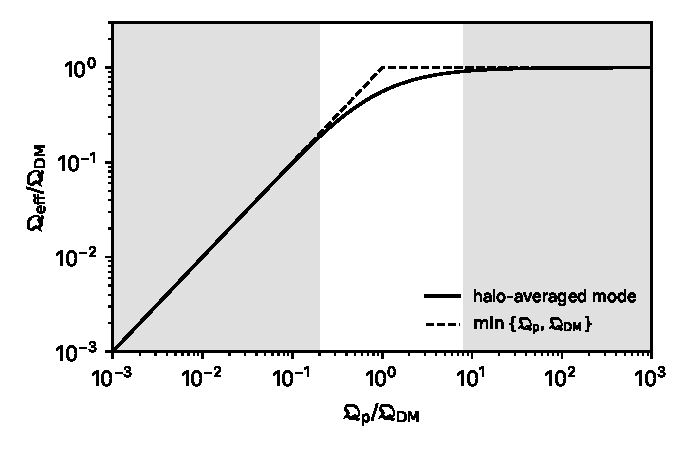
\includegraphics[width=0.8\linewidth]{figures/ch11/limit11_8b.pdf}
\captionof{figure}{Effective quality factor of a resonator mode in the halo field, \cref{eq:11.8-Qeff}, in units of $\mathfrak{Q}_{\mathrm{DM}} = 1.34\times10^6$, against the quality factor of the mode, $\mathfrak{Q}_{\mathrm{p}}/\mathfrak{Q}_{\mathrm{DM}}$, with the mode tuned to the frequency that maximizes it. Solid: \cref{eq:11.8-Qeff} with $F_\phi$ from the speed distribution of the standard halo of \cref{sec:1.2}; dashed: $\min\{\mathfrak{Q}_{\mathrm{p}}, \mathfrak{Q}_{\mathrm{DM}}\}$. Gray: $\mathfrak{Q}_{\mathrm{p}}/\mathfrak{Q}_{\mathrm{DM}} < 0.2$ and $> 7.9$, where the two agree within \SI{10}{\percent}. At $\mathfrak{Q}_{\mathrm{p}} = \mathfrak{Q}_{\mathrm{DM}}$ the prescription is 1.8 times too high.}\label{fig:11-limit-8b}
\par}
\smallskip
Where the widths of the mode and of the field are comparable, the signal is their convolution and neither width alone sets it; for records shorter than the coherence time the mean power is not a rate at all.
\end{limitbox}

The inputs that \cref{eq:11.8-Pn} needs are material and geometric. The elastic and piezoelectric tensors come from density-functional perturbation theory, and the shapes and frequencies of the modes of the actual body from finite elements. Add the shape factor $f_{\mathrm{sh}}$ of \cref{eq:11.8-shape} and the measured quality factor of the mode, which for acoustic resonators of this kind lies between $10^6$ and $10^{10}$~\cite{trickle2025piezoelectric}. A mode with $\mathfrak{Q}_{\mathrm{p}}$ above $10^7$ is in the narrow regime, where the signal is set by the field, not by the resonator. Its ring-down time, $\mathfrak{Q}_{\mathrm{p}}/\omega_n$, then exceeds the coherence time of the field, and the mean power of \cref{eq:11.8-Qeff} is reached only after many coherence times. How the signal builds up over shorter records, and how it fluctuates, is the coherent regime of \cref{sec:14.6}.

\subsection{Resonant-mass detectors}\label{sec:11.8-mass}

At masses of a peV to a neV the scalar of \cref{sec:11.8-gaas} does something else. Its coupling $g_{\phi ee}\phi\bar\psi\psi$ adds $-g_{\phi ee}\phi$ to the electron mass, and with $\phi = \phi_0\cos(m_\phi t)$, $\phi_0 = (2\rho_\chi)^{1/2}/m_\phi$, the electron mass oscillates, $\delta m_e/m_e = -g_{\phi ee}\phi/m_e$. A scalar coupled to $F_{\mu\nu}F^{\mu\nu}$ makes the fine-structure constant oscillate in the same way. Arvanitaki, Dimopoulos and Van Tilburg write both with dimensionless couplings normalized to the strength of gravity~\cite[Eqs.~(1), (3), (4)]{arvanitaki2016sound}. Such a field changes the size of every atom. The Coulomb Hamiltonian of electrons and clamped nuclei, \cref{eq:2.3-HC} with $M_\kappa \to \infty$, contains $\alpha$ and $m_e$ only through the Bohr radius $a_0 = 1/(\alpha m_e)$, which sets every length, and $\alpha^2m_e$, which sets every energy. The lattice constant is a fixed number of Bohr radii, and
\begin{equation}
  h_{\mathrm{mod}} \equiv \frac{\delta a}{a} = -\frac{\delta\alpha}{\alpha} - \frac{\delta m_e}{m_e} .
  \label{eq:11.8-h}
\end{equation}
The scaling fails only through physics that the Coulomb Hamiltonian leaves out. Relativistic corrections are of relative order $(Z\alpha)^2$ for the inner electrons. They add to $\dd\ln a/\dd\ln\alpha$ a term that fully relativistic calculations put at $-1.97\times10^{-2}$ for copper and $-2.2\times10^{-4}$ for silicon; the finite nuclear mass adds a dependence on the proton-to-electron mass ratio, $-1.12\times10^{-3}$ per unit fractional change for copper and $-0.86\times10^{-3}$ for silicon~\cite[Table~II]{pasteka2019material}. For a light crystal \cref{eq:11.8-h} holds to about $10^{-3}$.

A resonant-mass detector reads out such a change. It is a massive elastic body, a cylindrical bar or a sphere, of low internal loss, whose lowest mode is watched by a transducer at its own frequency. The detectors were built for gravitational waves, and the cryogenic ton-scale aluminum bars of the last generation ring near \SI{900}{Hz}~\cite{arvanitaki2016sound}, an energy of \SI{3.7}{peV}.

Why should an oscillating size excite a mode at all? A static change of $a$ excites nothing. The body simply takes its new equilibrium shape, with every material point $\vect{\xi}$ moved to $(1 + h_{\mathrm{mod}})\vect{\xi}$, and there is no wave. Write the displacement in the laboratory as $\vect{u}_{\mathrm{lab}} = \vect{u} + h_{\mathrm{mod}}(t)\,\vect{\xi}$, with $\vect{u}$ the displacement from the instantaneous equilibrium. The elastic stress responds to the strain relative to that equilibrium, $\sigma = C : (\nabla\vect{u}_{\mathrm{lab}} - h_{\mathrm{mod}}\mathbb{1}) = C : \nabla\vect{u}$, for a uniform $h_{\mathrm{mod}}$ in a cubic or isotropic body, with $C$ the elastic tensor. Newton's law holds in the laboratory, $\rho_T\ddot{\vect{u}}_{\mathrm{lab}} = \nabla\cdot\sigma$, and
\begin{equation}
  \rho_T\,\ddot{\vect{u}} = \nabla\cdot(C : \nabla\vect{u}) - \rho_T\,\ddot h_{\mathrm{mod}}\,\vect{\xi} .
  \label{eq:11.8-drive}
\end{equation}
The scalar acts as a body force $-\rho_T\ddot h_{\mathrm{mod}}\vect{\xi}$, the inertial force of the moving equilibrium. It is proportional to $\omega^2h_{\mathrm{mod}}$: the stiffness of the body never enters, and a slow modulation is followed adiabatically. Projected on a mode $\vect{u}_n$ of the body, the force is $F_n = -\ddot h_{\mathrm{mod}}\int\dd^3\xi\,\rho_T\,\vect{\xi}\cdot\vect{u}_n$. For a sphere of radius $R_{\mathrm{sph}}$ and mass $M_{\mathrm{sph}}$ only the radial modes $\vect{u}_n = \hat{\vect{r}}u_n(r)$ couple, and $F_n = -\ddot h_{\mathrm{mod}}M_{\mathrm{sph}}R_{\mathrm{sph}}J_n$ with $J_n = 3R_{\mathrm{sph}}^{-4}\int_0^{R_{\mathrm{sph}}}\dd r\,r^3u_n(r)$, which Arvanitaki and collaborators obtain by treating the modulus as a scalar gravitational wave with the curvature $\delta_{ij}\ddot h$~\cite[Eqs.~(7), (8)]{arvanitaki2016sound}.

A thin bar of length $L_{\mathrm{b}}$ and sound speed $c_{\mathrm{b}}$, free at both ends, shows the whole response in closed form. Along the bar, \cref{eq:11.8-drive} with $h_{\mathrm{mod}}\ee^{-\ii\omega t}$ has the solution $u_{\mathrm{lab}} = h_{\mathrm{mod}}\sin(k\xi)/[k\cos(kL_{\mathrm{b}}/2)]$, $k = \omega/c_{\mathrm{b}}$, which satisfies the free-end condition $\partial_\xi u_{\mathrm{lab}} = h_{\mathrm{mod}}$ at $\xi = \pm L_{\mathrm{b}}/2$. Measured from the instantaneous equilibrium, the end moves by
\begin{equation}
  u(L_{\mathrm{b}}/2) = \frac{h_{\mathrm{mod}}L_{\mathrm{b}}}{2}\Bigl(\frac{\tan x}{x} - 1\Bigr) , \qquad x = \frac{\omega L_{\mathrm{b}}}{2c_{\mathrm{b}}} = \frac{\pi}{2}\,\frac{\omega}{\omega_1} ,
  \label{eq:11.8-bar}
\end{equation}
with $\omega_1 = \pi c_{\mathrm{b}}/L_{\mathrm{b}}$ the lowest mode that couples. Below it, $\tan x/x - 1 \simeq x^2/3$, and the response is $(\pi^2/24)\,h_{\mathrm{mod}}L_{\mathrm{b}}(\omega/\omega_1)^2$, the $\omega^2$ of the drive. At each odd mode it resonates. Far above, the end stays where it was in the laboratory while the equilibrium moves, and the relative displacement tends to $-h_{\mathrm{mod}}L_{\mathrm{b}}/2$. The lowest mode alone, $u_1 = \sin(\pi\xi/L_{\mathrm{b}})$ with mass $M_{\mathrm{b}}/2$ and force $2\omega^2h_{\mathrm{mod}}M_{\mathrm{b}}L_{\mathrm{b}}/\pi^2$, gives $(4/\pi^2)h_{\mathrm{mod}}L_{\mathrm{b}}(\omega/\omega_1)^2/(1 - \omega^2/\omega_1^2)$; its low-frequency coefficient, $4/\pi^2 = 0.405$, falls short of $\pi^2/24 = 0.411$ by the higher odd modes, whose shares $4/\pi^2n^4$ sum to the difference.

\begin{limitbox}[Resonant-mass drive of a scalar][lim:11.8c]
A scalar that changes $\alpha$ or $m_e$ strains a body by $h_{\mathrm{mod}} = -\delta\alpha/\alpha - \delta m_e/m_e$ and drives its modes with the force $F_n = -\ddot h_{\mathrm{mod}}M_{\mathrm{sph}}R_{\mathrm{sph}}J_n$, proportional to $\omega^2$~\cite[Eqs.~(6)--(8)]{arvanitaki2016sound}.
\par\smallskip
{\centering
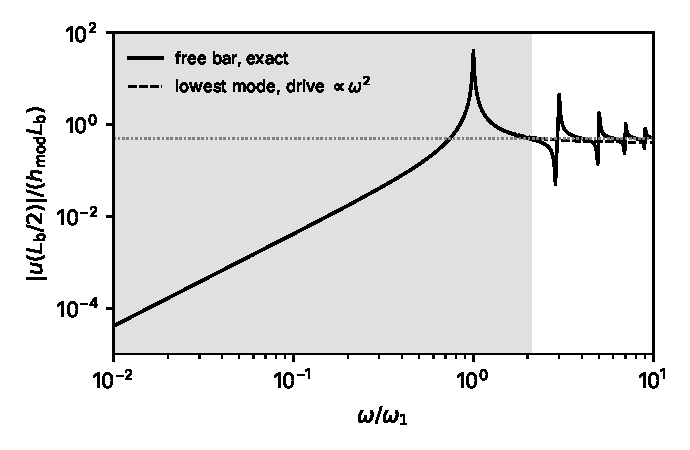
\includegraphics[width=0.8\linewidth]{figures/ch11/limit11_8c.pdf}
\captionof{figure}{Displacement of the end of a free bar from its instantaneous equilibrium, in units of $h_{\mathrm{mod}}L_{\mathrm{b}}$, against $\omega/\omega_1$. Solid: the exact response \cref{eq:11.8-bar}; dashed: the lowest mode alone with the $\omega^2$ drive. Every mode has the width $\omega_n/\mathfrak{Q}$ with $\mathfrak{Q} = 100$ for visibility (resonant-mass detectors reach $10^6$ to $10^7$). Dotted: the high-frequency limit $1/2$. Gray: $\omega < 2.1\,\omega_1$, where the lowest mode is within \SI{10}{\percent} of the exact response. The field is uniform over the bar while $m_\phi vL_{\mathrm{b}} \ll 1$. With $v = 10^{-3}$ and $c_{\mathrm{b}} = \SI{5}{km/s}$ this holds up to $\omega \approx 2\times10^7\omega_1$, far off scale.}\label{fig:11-limit-8c}
\par}
\smallskip
Above the lowest mode the higher modes and their antiresonances take over, and the response approaches the rigid limit, in which the body no longer follows its equilibrium.
\end{limitbox}

\section{Uncertainty budget of the lattice rates}\label{sec:11.9}

A dark-matter particle of \SI{30}{MeV} with a heavy mediator and $\sigma_p = 10^{-40}\,\mathrm{cm^2}$ makes $5.26\times10^3$ events per kilogram-year in silicon above a threshold of \SI{100}{meV}. The number assumes a harmonic crystal, nuclei that scatter independently and the phonons of the PBE force constants of \cref{sec:5.2}. The free nuclear recoil of the standard rate gives $4.91\times10^3$ for the same threshold, and above \SI{400}{meV} it gives a sixteenth of the crystal rate. That difference is the error of the simpler calculation: the crystal response is the better one, and the free recoil is its limit at large $x_R$ (\cref{sec:11.4}). The uncertainty is how far the crystal number moves when the truncations of this chapter are lifted, and \cref{tab:11-nuisances} lists these steps in the classes and bases of \cref{tab:10-nuisances}. A next order computed with the force constants of \cref{sec:5.2} or with measured inputs is marked ``computed'', and its central value has already moved.

The exact $\omega$-integrated weight of \cref{eq:11.3-weight} moves the central value of each phonon order; what remains is the distribution of the coherent weight in $\omega$ inside each band, which \cref{eq:11.3-band} bounds at every point but does not fix. The residual is a tilt within each band, and it matters for a threshold inside a band at momentum transfers below a few $q_{\mathrm{BZ}}$. Above the impulse onset the zeroth and first moments of the recoil spectrum are exact on any energy surface, and the anharmonic template is the constrained tilt \cref{eq:8.8-tilt}, which keeps them. For soft-mode and light-atom crystals, and for solid helium near melting, neither a computed next order nor a small parameter exists, and the Markov--Krein band of \cref{eq:C.10-band} is the only available statement (\cref{lim:11.5c}): a range without a central value, whose edges a likelihood uses.

The phonons themselves are an input, not a truncation of the label, and their error plays the part of the spread between tabulations in \cref{sec:10.10}. Of the eight measured frequencies of silicon at $\mathrm{\Gamma}$, X and L, the PBE force constants of \cref{sec:5.2} miss by \SI{2.6}{\percent} on average and the zone-center optical mode by \SI{0.6}{\percent}. We take as template a uniform rescaling of all phonon frequencies by \SI{2.6}{\percent}. It moves the Poisson weights through $2W_\kappa \propto \langle\omega^{-1}\rangle$ and the impulse width through $\langle\omega\rangle^{1/2}$ together, and since the deviations of single modes have both signs, it is an upper template. The measured elastic tensors that fix the acoustic plateau and edge of \cref{sec:11.1} are room-temperature values, and the change on cooling has not been sized.

\begin{table}[tbp]
  \caption{Uncertainty budget of the lattice rates. Classes and bases as in \cref{tab:10-nuisances}. Sizes are for silicon unless another crystal is named; \cref{we:11-band30} is the silicon rate at \SI{30}{MeV} above \SI{100}{meV}, and $d$ the site difference of \cref{we:11-gaas}. Items without a row: the optical-phonon shift of \SI{0.15}{meV} (\cref{tab:8-nuisances}), the quantum-crystal and germanium-spectrum models (\cref{sec:11.4,sec:11.5}), the absorption line widths and resonator prescription (\cref{sec:11.8}), and the nuclear spin inputs.}
  \label{tab:11-nuisances}
  \centering\footnotesize\setlength{\tabcolsep}{3pt}
  \begin{tabular}{@{}>{\raggedright\arraybackslash}p{0.25\linewidth}>{\raggedright\arraybackslash}p{0.12\linewidth}>{\raggedright\arraybackslash}p{0.38\linewidth}>{\raggedright\arraybackslash}p{0.09\linewidth}>{\raggedright\arraybackslash}p{0.10\linewidth}@{}}
    \toprule
    Truncation or input & Type & Size & Basis & Section \\
    \midrule
    Pairs of nuclei dropped (incoherent approximation) & normali\-zation per order & within \SI{10}{\percent} above \SI{6.6}{keV} ($n = 2, 3$); \cref{we:11-band30}: $+2.6\times10^{-4}$ & computed & \cref{sec:11.3} \\
    Coherent weight inside a band & tilt & up to $2.7\times$ incoherent at \SI{10}{keV} & bound & \cref{sec:11.3} \\
    Phonon frequencies (PBE) & tilt & \SI{2.6}{\percent} mean, uniform rescale (upper estimate); \cref{we:11-band30}: $+0.24\,\%$ ($+3.1\,\%$ above \SI{400}{meV}) & spread & \cref{sec:5.2} \\
    Anharmonic recoil width, skewness ($n_A = 2$) & tilt (con\-strained) & kinetic energy within $\pm0.2\,\%$; third cumulant $\sim\eta_{\mathrm{anh}}^2$ & model; est. & \cref{sec:11.5} \\
    Anharmonic few-phonon weights ($n_A = 2$) & tilt in $q$ & $n = 2$: $+\SI{50}{\percent}$, $n = 4$: $27\times$ at $q_{\mathrm{BZ}}$; harmonic to \SI{10}{\percent} above 5, 12, \SI{20}{keV} & model & \cref{sec:11.5} \\
    Strong anharmonicity (soft modes, light atoms, helium) & any & Markov--Krein band; Si, \SI{100}{keV}: 0.19 to 0.86 at $E_R$ & bound & \cref{sec:11.5} \\
    Thermal diffuse scattering ($n_T = 2$) & new support & $\propto T^2$; $10^{-9}$ of room temperature at \SI{10}{mK} & model & \cref{sec:11.3} \\
    Charge vertex above the zone & tilt in $q$ & unknown at 3--\SI{20}{keV}; nucleon coupling unaffected & named & \cref{sec:11.3} \\
    Free recoil for the crystal (evaluation error) & tilt & \SI{10}{\percent} from $x_R = 2.3$ (\SI{1}{GeV}); \cref{we:11-band30}: $-6.8\,\%$, $\times0.062$ above \SI{400}{meV} & computed & \cref{sec:11.4} \\
    Sound speeds & normali\-zation; threshold & computed against measured tensors & spread & \cref{sec:17.5} \\
    $Z^*/\varepsilon_\infty$, polar rates & normali\-zation & splitting route: rate \SI{2}{\percent}; semilocal $\varepsilon_\infty$: $-37\,\%$ & spread & \cref{sec:11.2} \\
    Charge of acoustic waves & new support & at most \SI{3}{\percent} near the edge, \SI{1}{\percent} at \SI{100}{keV} (GaAs); quadrupoles not computed & est. & \cref{sec:11.2} \\
    $Z^*/\varepsilon_\infty$, GaAs scalar absorption & normali\-zation & \SI{1}{\percent} gives \SI{9}{\percent}; PBE inputs: $/250$ & spread & \cref{sec:11.8} \\
    Core kinetic energy; mean masses (GaAs scalar) & normali\-zation & $\Delta d \approx -0.1\,d$, rate $-\SI{19}{\percent}$ (parametric); \SI{0.01}{u}: \SI{5}{\percent} of $d$ & est. & \cref{sec:11.8} \\
    Single-isotope density of states & normali\-zation & $+\SI{8.0}{\percent}$ at \SI{50}{meV} & computed & \cref{sec:11.6} \\
    Cold in-band absorption of silicon & normali\-zation & $\varGamma_{\mathrm{iso}}/\varGamma_{\mathrm{EM}} \ge 5.0\times10^3$; warm datum \SI{10}{\percent} & bound & \cref{sec:11.6} \\
    Electronic cubic harmonics & tilt in time & Si $A_{\mathrm{day}} = \SI{0.9}{\percent}$ without local fields & model & \cref{sec:11.7} \\
    \bottomrule
  \end{tabular}
\end{table}

A truncation that two rates share carries one parameter in both (\cref{sec:8.8}). The phonon frequencies of one set of force constants enter the one-phonon, multiphonon and impulse rates of that crystal together, at every mass and threshold, and a fit that gave each its own $\vartheta$ would let the data trade them. The measured elastic tensor of \cref{sec:11.1} is a different input, and an acoustic rate built from it shares no parameter with the multiphonon rate built from computed phonons. The ratio $Z^*/\varepsilon_\infty$ of a polar crystal is one input of its dark-photon scattering rate, its dark-photon absorption and its electron-scalar absorption, and one $\vartheta$ moves all three, by different factors. The halo stays fixed, as in \cref{eq:8.8-like}, and the detector uncertainties belong to \cref{sec:21.4}.

\begin{workedexample}{The uncertainty band of the silicon multiphonon rate at \SI{30}{MeV}}\label{we:11-band30}
Take $\mchi = \SI{30}{MeV}$, a heavy mediator, equal couplings to protons and neutrons with $\sigma_p = 10^{-40}\,\mathrm{cm^2}$, and the standard halo of \cref{sec:1.2} with $\rho_\chi = \SI{0.3}{GeV.cm^{-3}}$. The threshold $\omega_{\mathrm{th}} = \SI{100}{meV}$ and the cross-section $\sigma_p$ are illustrative choices; the threshold lies above the one-phonon band, so that every event counted contains at least two phonons. The largest momentum transfer is $2\mchi v_{\mathrm{max}} = \SI{159}{keV}$, where $E_R = \SI{0.48}{eV}$ and $x_R = 11.8$. The central value is \cref{eq:8.2-spectrum} with one row and the incoherent harmonic response of all orders at $T = 0$, from the PBE density of states of \cref{sec:5.2}, the Helm form factor, and the velocity integral done for an orientation-averaged crystal:
\begin{equation*}
  \mathcal{R}^{\mathfrak{T}} = \SI{5.26e3}{kg^{-1}.yr^{-1}} ,
\end{equation*}
with $\mathcal{R}^{\mathfrak{T}}$ the rate at the central values of the truncation labels (\cref{sec:10.10}), or 14 events per kilogram and day. Half of it comes from momentum transfers below \SI{80}{keV}, where $x_R = 3.0$, and \SI{80}{\percent} from between 54 and \SI{109}{keV}, $x_R$ from 1.4 to 5.6: the rate spans the impulse onset.

The computed coherent step multiplies each phonon order by $1 + \delta^{\mathrm{coh}}_n(q)$ from \cref{eq:11.3-weight}. Between 30 and \SI{159}{keV}, $|\delta^{\mathrm{coh}}_2|$ stays below 0.021 and $|\delta^{\mathrm{coh}}_8|$ below $1.5\times10^{-4}$, and the rate rises by $2.6\times10^{-4}$, which leaves $5.26\times10^3$ unchanged at three digits. The remaining uncertainties enter the power form \cref{eq:8.8-M} through $\ln(1 + \delta_k)$:
\begin{equation*}
  \begin{aligned}
  &\text{phonon frequencies, } +\SI{2.6}{\percent}: & \ln(1 + \delta) &= +2.4\times10^{-3}, \\
  &\text{anharmonic kinetic energy, } -\SI{0.14}{\percent}\ (\lambda_3 = 0.01, & &-8\times10^{-5}, \\
  &\qquad\lambda_4 = 2.5\times10^{-4}): & & \\
  &\text{anharmonic third cumulant (est.)}: & &+5\times10^{-5}.
  \end{aligned}
\end{equation*}
The kinetic-energy template is a dilation of each spectrum about $E_R$ by $(1 + \delta E^{\mathrm{kin}}/E^{\mathrm{kin}})^{1/2}$, which keeps the area and the mean and changes the second moment by the computed amount; the rate changes by 0.12 times the relative change of the width, and the extreme $-\SI{0.2}{\percent}$ of the range of \cref{sec:11.5} would give $-1.2\times10^{-4}$. For the third cumulant, the whole difference between the incoherent spectrum and a Gaussian of the same mean and variance changes the rate by \SI{1.9}{\percent}, and the anharmonic change of the cumulants is of relative order $\eta_{\mathrm{anh}}^2$. The anharmonic few-phonon weights barely enter: below \SI{20}{keV}, where they are large, $E_R$ is under \SI{8}{meV}, and those momentum transfers carry $3\times10^{-4}$ of the rate. With independent standard-normal $\vartheta_k$ the widths add in quadrature, \cref{eq:C.14-quadrature},
\begin{equation*}
  \sigma_{\ln\mathcal{R}} = \bigl[(2.4\times10^{-3})^2 + (8\times10^{-5})^2 + (5\times10^{-5})^2\bigr]^{1/2} = 2.4\times10^{-3} ,
\end{equation*}
and the rate lies between $5.25\times10^3$ and $5.27\times10^3$ per kilogram-year at one standard deviation, a factor of 1.0024 either way. The phonon frequencies carry all of it.

The free recoil gives $4.91\times10^3$, \SI{6.8}{\percent} lower, 29 band widths away. With the threshold raised to \SI{400}{meV}, near the endpoint \SI{0.48}{eV}, the crystal rate falls to \SI{110}{kg^{-1}.yr^{-1}}, half of it from momentum transfers below \SI{118}{keV}, $x_R = 6.5$. The free recoil gives 6.8, a sixteenth of it, because above \SI{400}{meV} most events come from the Doppler tail of the recoil spectrum, which the free nucleus does not have. The rate now samples the width of that spectrum, the dilation coefficient grows from 0.12 to 2.2, and the frequency template becomes $+\SI{3.1}{\percent}$; the band is a factor of 1.031. The anharmonic kinetic energy gives $-1.5\times10^{-3}$, still a twentieth of it.

Without perturbation theory the same rate would be far less certain. At \SI{80.4}{keV}, the median momentum transfer of the rate above \SI{100}{meV}, the five exact moments of the response allow any weight above threshold between 0.19 and 0.95 by the Markov--Krein band, against the harmonic 0.58.
\end{workedexample}

\section*{Summary}

A nucleon-coupled particle too light to give a nucleus a free recoil above threshold excites phonons, because the whole crystal takes up the momentum (\cref{sec:11.1}). At momentum transfers well inside the zone the one-phonon response per unit mass depends on the material only through the sound speeds and polarizations of the acoustic branches. The acoustic edge, set by the fastest longitudinal sound speed, \SI{6.1}{keV} for silicon at a \SI{1}{meV} threshold, lies 21 times above the free-target threshold mass. For a heavy mediator the rate reaches a plateau proportional to the polarization-weighted inverse sound speed, 654 events per kilogram and year in silicon at $\sigma_p = 10^{-40}\,\mathrm{cm^2}$.

A dark photon couples to charge and, in a polar crystal, excites the longitudinal optical phonon through the screened Born charge (\cref{sec:11.2}); for GaAs $Z^*/\varepsilon_\infty = 0.194$ from the measured splitting. Above the zone a nucleus leaves behind several phonons, Poisson distributed in the self part of the response, and the exact $\omega$-integrated weight, a static sum over pairs, corrects the incoherent approximation at every momentum transfer (\cref{sec:11.3}). At large momentum transfer the phonon orders merge into one peak at $E_R$ (\cref{sec:11.4}). At \SI{100}{keV} in silicon it lies at \SI{191}{meV} and is \SI{88}{meV} wide, and the free nuclear recoil with the Helm form factor, its limit, holds for a heavy particle within \SI{10}{\percent} from $x_R = 2.3$. In a crystal the free-nucleus formula for fermionic absorption on nuclei overstates the rate 16 times at \SI{10}{keV}.

Anharmonicity enters the rate first at second order, by time reversal (\cref{sec:11.5}); in silicon it changes the impulse width by less than a part in a thousand, and strongly anharmonic targets at detector temperatures have only the Markov--Krein band. Couplings that change from site to site give a broadband response that follows the density of states (\cref{sec:11.6}), and through the isotopes a baryon-minus-lepton vector is absorbed in silicon at least $5.0\times10^3$ times faster than through the electromagnetic channel at \SI{50}{meV}. A silicon crystal at $45^\circ$N modulates by \SI{0.9}{\percent} in its electronic rate and \SI{0.58}{\percent} in its lattice rate at \SI{2}{MeV} over the sidereal day (\cref{sec:11.7}). At neV to \si{\micro eV} masses the field is coherent over the body, and the acoustic modes of a resonator absorb it (\cref{sec:11.8}).

At \SI{30}{MeV} with a heavy mediator the silicon rate above \SI{100}{meV} is $5.26\times10^3$ events per kilogram-year, uncertain by a quarter of a percent, almost all of it from the computed phonon frequencies (\cref{sec:11.9}). The polar rates are set by $Z^*/\varepsilon_\infty$, which a computed $\varepsilon_\infty$ misses by enough to move a rate by \SI{37}{\percent}. Throughout the chapter the electrons stayed in their ground state and followed the nuclei. When a nucleus is kicked they do not follow at once, and \cref{chap:12} computes how often a nuclear recoil also excites them.

\printbibliography[heading=subbibliography]
